% The main file for developing the proposal. 
% Variants with different class options are 
% - submit.tex (no draft stuff, no ednotes, no revision information)
% - public.tex (like submit.tex, but no financials either) 
\providecommand{\classoptions}{} % to be overwritten in variants
\documentclass[12pt,noworkareas,deliverables,report,notecites,longtasklabels,submit\classoptions]{euproposal}
\extrafloats{1000}

\usepackage{nimbusserif}
\usepackage{logipedia}
\usepackage{framed}
\usepackage{multicol}
\usepackage{longtable}
\usepackage{array}
\let\ganttchart\undefined
\usepackage{pgfgantt}

% color set x11names
% see http://mirrors.ctan.org/macros/latex/contrib/xcolor/xcolor.pdf
% p. 39-40
%\definecolor{color1}{RGB}{254,248,108}
\definecolor{color1}{RGB}{250,234,115}
\definecolor{color2}{named}{DarkSeaGreen1}
\definecolor{color3}{named}{SteelBlue1}

\addbibresource{lib/kbibs/kwarcpubs.bib}
\addbibresource{lib/kbibs/extpubs.bib}
\addbibresource{lib/kbibs/kwarccrossrefs.bib}
\addbibresource{lib/kbibs/extcrossrefs.bib}
\addbibresource{lib/pub_rabe.bib}
\addbibresource{lib/rabe.bib}
\addbibresource{lib/proposal.bib}
\addbibresource{lib/interface.bib}

\WAperson[id=GiDo, 
           personaltitle=Prof. Dr.,
           academictitle=Professor of ????,
           affiliation=Inr,
           email=gilles.dowek@ens-paris-saclay.fr,
           workaddress={????},
           worktel=?????]
           {Gilles Dowek}

% institutions in the same order as on the submission website

\WAinstitution[id=Inr,
        countryshort=FR,
        acronym=Inr]
        {Institut National de Recherche en Informatique et Automatique}

\WAinstitution[id=Str,
        countryshort=FR,
        acronym=Str]
        {Université de Strasbourg}

\WAinstitution[id=Tou,
        countryshort=FR,
        acronym=Tou]
        {Institut National Polytechnique de Toulouse}

\WAinstitution[id=Inn,
        countryshort=AT,
        acronym=Inn]
        {Universität Innsbruck}

\WAinstitution[id=Lie,
        countryshort=BE,
        acronym=Lie]
        {Université de Liège}

\WAinstitution[id=Bol,
        countryshort=IT,
        acronym=Bol]
        {Alma Mater Studiorum – Università di Bologna}

\WAinstitution[id=Pra,
        countryshort=CZ,
        acronym=Pra]
        {České vysoké učení technické v Praze}

\WAinstitution[id=Bel,
        countryshort=RS,
        acronym=Bel]
        {Faculty of Mathematics, University of Belgrade}

\WAinstitution[id=Tum,
        countryshort=DE,
        acronym=Tum]
        {Technische Universität München}

\WAinstitution[id=Del,
        countryshort=NL,
        acronym=Del]
        {Technische Universiteit Delft}

\WAinstitution[id=Sac,
        countryshort=FR,
        acronym=Sac]
        {Université Paris-Saclay}

\WAinstitution[id=Fau,
        countryshort=DE,
        acronym=Fau]
        {Friedrich-Alexander Universit\"at Erlangen-N\"urnberg}

\WAinstitution[id=Lee,
        countryshort=UK,
        acronym=Lee]
        {University of Leeds}

\WAinstitution[id=Sou,
        countryshort=UK,
        acronym=Sou]
        {University of Southampton}

\WAinstitution[id=Got,
        countryshort=SE,
        acronym=Got]
        {G\"oteborgs Universitet}

\WAinstitution[id=Cha,
        countryshort=SE,
        acronym=Cha]
        {Chalmers Tekniska H\"ogskola}

\WAinstitution[id=Lmu,
        countryshort=DE,
        acronym=Lmu]
        {Ludwig-Maximilians-Universit\"at M\"unchen}

\WAinstitution[id=Ipp,
        countryshort=FR,
        acronym=Ipp]
        {Ecole Polytechnique}

\WAinstitution[id=Imt,
        countryshort=FR,
        acronym=Imt]
        {Institut Mines-Télécom}

\WAinstitution[id=Bia,
        countryshort=PL,
        acronym=Bia]
        {Uniwersytet w Białymstoku}

\WAinstitution[id=Dus,
        countryshort=DE,
        acronym=Dus]
        {Heinrich-Heine-Universität Düsseldorf}

\WAinstitution[id=Cle,
        countryshort=FR,
        acronym=Cle]
        {ClearSy}

\WAinstitution[id=Oca,
        countryshort=FR,
        acronym=Oca]
        {OCamlPro}

\WAinstitution[id=Fac,
        countryshort=FR,
        acronym=Fac]
        {Facebook France}

\WAinstitution[id=Bir,
        countryshort=UK,
        acronym=Bir]
        {University of Birmingham}

\WAinstitution[id=Min,
        countryshort=FR,
        acronym=Min]
        {Association pour la Recherche et le Développement des Méthodes et Processus Industriels}

\WAinstitution[id=Cea,
        countryshort=FR,
        acronym=Cea]
        {Commissariat à l'Energie Atomique et aux Energies Alternatives}

\WAinstitution[id=Stu,
        countryshort=DE,
        acronym=Stu]
        {Duale Hochschule Baden-Württemberg}
        
%%% Local Variables: 
%%% TeX-master: "../propB"
%%% mode: latex
%%% End: 

% LocalWords:  WAperson miko personaltitle academictitle privaddress privtel
% LocalWords:  workaddress worktel workfax gc worktelfax pcg pcsa WAinstitution
% LocalWords:  shortname partof streetaddress townzip countryshort efo 3kd89
% LocalWords:  jacobs-logo.png Seefahrtstrasse Kruislann Montparnasse Universit
% LocalWords:  baz Westerfield
% Some sections of the included files depend on this.

\counterwithout{figure}{chapter}
\renewcommand\chaptername{Section}

\begin{document}
{\color{red} version du 13 mars à 12:23}% modified by Frédéric only

\begin{proposal}[%
  coordinator=GiDo,
  coordinatorsite=Inr,
  acronym={Logipedia},
  acrolong={},
  title=\pn \protect\pnlong, % sites in the order of the submission site
  site=Inr,
  site=Str,
  site=Tou, 
  site=Inn, 
  site=Lie,
  site=Bol,
  site=Bel,
  site=Tum,
  site=Del, 
  site=Sac, 
  site=Fau,
  site=Lee,
  site=Got,
  site=Cha,
  site=Lmu,
  site=Imt,
  site=Bia,
  site=Oca,
  site=Cle,
  site=Bir,
  site=Cea,
  site=Stu,
  site=Edu,
  site=Med,
  site=Pro,
  site=Zib,
  site=Ias,
  site=Run,
  botupPM, % we want to work via bottom up PM distribution,
  % alternative: (can be combined)
  % topdownPM, % the coordinator distributes PM as follows:
  % FAURM=72,
  callname = Integrating and opening research infrastructures\\ of European interest,
  callid = H2020-INFRAIA-2018-2020,
  instrument=instrument,
  challengeid=challengeid,
  challenge=challenge,
  objectiveid=objectiveid,
  objective=objective,
  months=48,
  compactht]

  \thispagestyle{empty}
  \newcommand\ap{{\color{SpringGreen3}$\bullet$}}% academic partner
  \newcommand\ip{{\color{OrangeRed1}$\star$}}% industrial partner

  \begin{center}
    {\Large\bf Integrating and opening research infrastructures\\of European interest}\\[10mm]

    {\LARGE H2020-INFRAIA-2018-2020}\\[10mm]

    \fbox{\LARGE\bf Logipedia}\\[10mm]

    Coordinator: Gilles Dowek (gilles.dowek@inria.fr)\\[10mm]
    
  \begin{tabular}{|c|l|l|c|c|}\hline
    \# & Partner organisation name & Short name & Country & Type\\\hline
    1 & Institut National de Recherche en Informatique et Automatique & Inria & FR & \ap\\\hline
    2 & Université de Strasbourg & Unistra & FR & \ap\\\hline
    3 & Institut National Polytechnique de Toulouse & INPT & FR & \ap\\\hline
    4 & Universität Innsbruck & UIBK & AT & \ap\\\hline
    5 & Université de Liège & ULiege & BE & \ap\\\hline
    6 & Alma Mater Studiorum – Università di Bologna & Unibo & IT & \ap\\\hline
    7 & Faculty of Mathematics, University of Belgrade & UBel & RS & \ap\\\hline
    8 & Technische Universität München & TUM & DE & \ap\\\hline
    9 & Technische Universiteit Delft & TUDelft & NL & \ap\\\hline
    10 & Université Paris-Saclay & USaclay & FR & \ap\\\hline
    11 & Friedrich-Alexander Universit\"at Erlangen-N\"urnberg & FAU & DE & \ap\\\hline
    12 & University of Leeds & ULeeds & UK & \ap\\\hline
    13 & G\"oteborgs Universitet & UGot & SE & \ap\\\hline
    14 & Chalmers Tekniska H\"ogskola & Chalmers & SE & \ap\\\hline
    15 & Ludwig-Maximilians-Universit\"at M\"unchen & LMU & DE & \ap\\\hline
    16 & Institut Mines-Télécom & IMT & FR & \ap\\\hline
    17 & Uniwersytet w Białymstoku & UBia & PL & \ap\\\hline
    18 & ClearSy & ClearSy & FR & \ip\\\hline
    19 & OCamlPro & OCamlPro & FR & \ip\\\hline
    20 & University of Birmingham & UoB & UK & \ap\\\hline
    21 & Commissariat à l'Energie Atomique et aux Energies Alternatives & CEA & FR & \ip\\\hline
    22 & Duale Hochschule Baden-Württemberg & DHBW & DE & \ap\\\hline
    23 & Edukera & Edukera & FR & \ip\\\hline
    24 & MED-EL Elektromedizinische Geraete GmbH & MED-EL & AT & \ip\\\hline
    25 & Prove \& Run & P\&R & FR & \ip\\\hline
    26 & Konrad-Zuse-Zentrum für Informationstechnik Berlin & ZIB & DE & \ap\\\hline
    27 & Universitatea Alexandru Ioan Cuza din Iasi & UAIC & RO & \ap\\\hline
    28 & Runtime Verification SRL & RV & RO & \ip\\\hline
  \end{tabular}

  \bigskip
  \ap~Academic partner \quad\quad \ip~Industrial partner
  \end{center}

  \newpage
  \begin{center}
    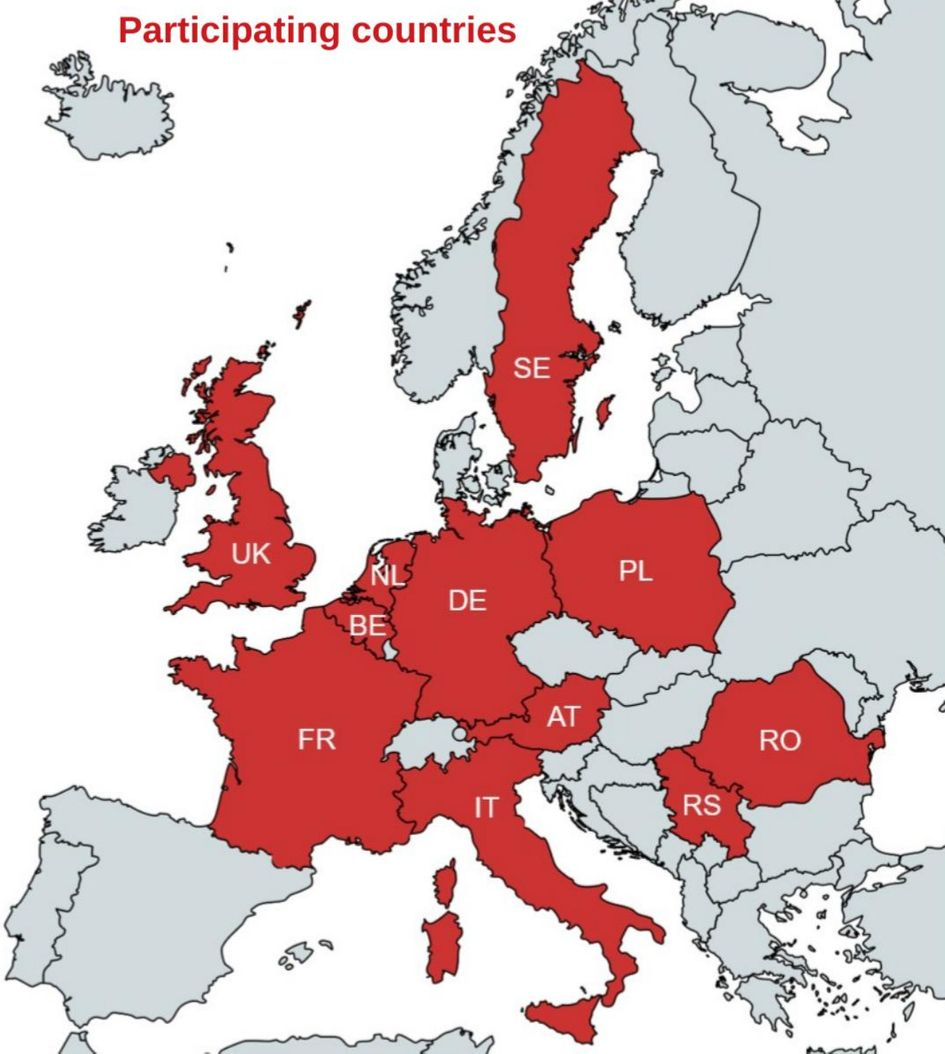
\includegraphics[width=8cm]{img/Map-reduced.jpg}
  \end{center}

  \vspace*{5mm}
  \begin{center}
    {\Large\bf Companies willing to join\footnote{Their letters of intent are at the end of the document for section 4-5.} the club of industrial users:}
  \end{center}

  \newcommand\logo[2][28mm]{\includegraphics[width=#1]{logos/#2}}
  
  \vspace*{5mm}
  \begin{tabular}{ccccc}% in alphabetical order
    \logo{Alstom}
    & \logo{ARM}
    & \logo[22mm]{CEAList}
    & \logo{ClearSy}
    & \logo{Edukera}
    \\[8mm]
    \logo{Facebook}
    & \logo{IBM}
    & \logo{MED-EL}
    & \logo{MERCE}
    & \logo{NomadicLabs}
    \\[5mm]
    \logo{OCamlPro}
    & \logo{Onera}
    & \logo{OriginLabs}
    & \logo[22mm]{ProveRun}
    & \logo{RATP}
    \\[13mm]
    \logo{RV}
    & \logo{Siemens}
    & \logo{Systerel}
    & \logo{Thales}
    & \logo{TrustedLabs}
    \\[11mm]
    \logo{TrustInSoft}
  \end{tabular}

  \newpage\null\vfil

\medskip
\hspace{-0.8cm}
\begin{tabular}{p{0.3\textwidth}p{0.7\textwidth}}
\begin{minipage}{0.3\textwidth}
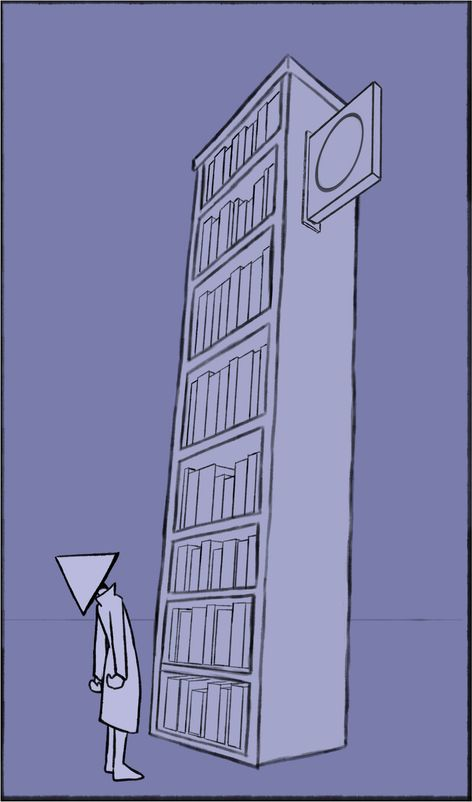
\includegraphics[width=4cm]{img/Illustration1-reduced.jpg}
\end{minipage}
&
\begin{minipage}{10cm}
  \begin{center}\bfseries Abstract\end{center}
    max 2000 characters

    the objectives of the proposal

    how they will be achieved

    their relevance to the work programme

    will be used as the short description  of the proposal in the evaluation process and in communications  with the programme management committees and other interested parties

    do not include any confidential information

    use plain typed text, avoiding formulae and other special characters

    use e-infrastructure

    key-words: 200 characters max
\end{minipage}
\end{tabular}

  \vfil\null\newpage
  \tableofcontents

\chapter{Excellence}
\thispagestyle{empty}

Bugs kill.  If testing software allows the presence of bugs to be
revealed, only formal verification can guarantee their absence.
Thus, the
trust in critical systems today relies on formal verification, in
particular formal proofs, that guarantee the safety of people
using transportation systems (autonomous cars, subways, trains,
planes, etc.), health systems (robotic surgery, ear implants, etc.), energy provided
by nuclear plants, financial applications, e-governance, etc.  We
should never fly in an autonomous plane driven by a piece of software
that has not been formally verified.

This crucial role of formal proof is highlighted by several successes,
like the correctness proofs of the automatic Paris metro line 14
\cite{Behm98,Lecomte17}, the detect-and-avoid system for unmanned aircraft
system developed by NASA \cite{Munoz16}, the operating system seL4
\cite{Klein09}, or the C compiler CompCert \cite{Leroy06}.  It has
been empirically observed that operating systems and compilers
often
have bugs, but proved systems and compilers, such as seL4 or CompCert, have
none, or
much fewer.  This is why, at the highest Evaluation Assurance Levels (EAL)
of the Common Criteria (CC) security evaluation international standard, in
effect since 1999, certification processes require proofs, and not
only testing.

Because a bug can cause people to die and companies to go bankrupt,
formal methods are crucial in the development of the information
society. Making formal methods more accessible to companies, via
better theories, better tools and better-training of workers, can
bring a significant competitive advantage to Europe.  Hence it is
crucial for Europe to master this technology and its evolution.

Proofs have also always been the basis of mathematics, and hence of
many mathematised sciences, and several important advances, are based
on formal proofs, such as the proof of the Feit-Thompson theorem
\cite{Gonthier13} and Hales' theorem (Kepler's conjecture)
\cite{Hales17}, show the wide range of applications of formal proofs,
from safety and security of software to mathematics.

These formal proofs are developed using research infrastructures called
``proof systems''.  These proof systems allow computer scientists,
mathematicians, engineers, and logicians to build and study formal
proofs, just like particle accelerators allow physicists to build and
study particles.  Some twenty major proof systems exist in the world
(Figure \ref{systems}).

%%%%%%%%%%%%%%%%%%%%%%%%%%%%%%%%%%%%%%%%%%%%%%%%%%%%%%%%%%%%%%%%%%%%%%%%%%%%%%
\begin{figure}[ht]
\definecolor{shadecolor}{named}{color1}
\begin{shaded}
\begin{center}
    {\bf \Large Major proof systems}\\[3mm]

\begin{tabular}{l@{\hspace{3cm}}l}
Abella                & Acl2\\
\underline{Agda}      & \underline{HOL Light}\\
\underline{Atelier B} & IMPS\\
\underline{Coq}       & Lean\\
\underline{FoCaliZe}  & \underline{LFSC}\\
\underline{HOL4}      & Nuprl\\
\underline{Isabelle}  & \underline{PVS}\\
\underline{KProver}  & \underline{TSTP}\\
\underline{Matita}\\
\underline{Minlog}\\
\underline{Mizar}\\
ProB\\
\underline{ProvenTools}\\
\underline{Rodin}\\
\underline{TLA+}\\
\underline{Why3}\\
\end{tabular}
\end{center}
\vspace{-5mm}\caption{The European ones are in the first column.
  Those addressed in the project are underlined\label{systems}}
\end{shaded}
\end{figure}

%%%%%%%%%%%%%%%%%%%%%%%%%%%%%%%%%%%%%%%%%%%%%%%%%%%%%%%%%%%%%%%%%%%%%%%%%%%%%%

A lot of formal proofs developed for one critical system could be used
in another.  Unfortunately, the development of formal methods is
slowed down by the large number of proof systems (and sometimes the
large number of versions, over time, of one single system) and the
lack of a common theory used by these systems.  For instance, the
Paris metro line 14 has been proved correct in Atelier B, while the
Nasa detect-and-avoid system for unmanned aircraft system has been
proved correct in PVS, the seL4 operating system has been proved
correct in Isabelle/HOL, and the compiler CompCert has been proved
correct in Coq.  Some projects, such as the proof of Hales' theorem,
have been started in different systems and required significant
integration efforts for obtaining the overall result.

Thus, the development of formal methods is slowed down by the lack of
integration of these research infrastructures.  Because of this lack
of integration, each small community is centered around one theory and
one system. Each library is specific to one proof system, or often
even to a specific version of this system. In general, a library
developed in one system cannot be used in another, and when the system
is no longer maintained, the library may disappear.  Thus,
interoperability (the possibility for one user to use a proof
developed in another system), sustainability (the possibility to use a
proof decades after it has been developed), and cross-verification
(the possibility to verify a proof in a system different from the ones in
which it has been constructed resulting in a higher assurance of its
correctness) are restricted.

The fragmentation of these infrastructures hinders productivity
because foundational work (for instance, developing a calculus library
with theorems about the sinus and cosinus functions, derivatives,
etc.) has to be repeated instead of being reused.  It also limits the
dissemination of formal proofs in non-specialist communities. For
instance, teaching formal proving to undergraduate students in a logic
course is difficult, as it requires the choice of a specific language,
a specific theory and a specific system that restrict the scope of the
course, instead of giving students the tools that are useful
everywhere. The same is true for the use of formal proofs in industry
or by working mathematicians.

On philosophical grounds, while we had in the past an (informal) proof
of Pythagoras' theorem or Fermat's little theorem, the same proof now
has different formalizations in PVS, Isabelle/HOL, Coq, etc.  Thus,
the universality of logical truth itself is jeopardized.  As we shall
see, it is not the first time in history that this universality of
logical truth is jeopardized: it already has been, for instance, in
the 19$^{\mbox{\footnotesize th}}$ century, with the non-Euclidean
geometries. This crisis of the non-Euclidean geometries has been
solved at the beginning of the 20$^{\mbox{\footnotesize th}}$ with the
invention of a logical framework: predicate logic
\cite{HilbertAckermann}, in which the various geometries could be
defined.

%%%%%%%%%%%%%%%%%%%%%%%%%%%%%%%%%%%%%%%%%%%%%%%%%%%%%%%%%%%%%%%%%%%%%%%%%%%%%%
\begin{center}
$\bigstar$ $\bigstar$ $\bigstar$
\end{center}

Making proof systems interoperable would avoid duplication of work,
reduce development time, enable cross-verification, and make formal
proofs accessible to a much larger community.  After three decades
dedicated to the development of these systems, allowing such a
cooperation between systems is the next step in the development of the
formal proof technology.

Each proof system comes with its own libraries, and these libraries
are also part of research infrastructures. To address the challenge of
improving cooperation between these proof systems, we will integrate
these libraries in an online encyclopedia of formal proofs. Each proof
in this encyclopedia will have versions in each theory where it can be
expressed, so that it can be used in as many systems as possible.

Each proof system implements a different theory. So Logipedia will
contain proofs expressed in different theories.  Such a
theory-independent infrastructure is made possible, because the
theories implemented in these different proof systems can be expressed
in a common logical framework: the $\lambda \Pi$-calculus modulo
theory, implemented in the system
\href{https://deducteam.github.io/}{Dedukti}. Dedukti is thus the {\em
  lingua franca} that permits this theory-independent encyclopedia to
exist.

{\bf Building such an encyclopedia will thus allow interoperability,
  sustainability, and cross-verification of all formal proofs in the
  encyclopedia.}

This encyclopedia will be called Logipedia.

Logipedia is thus a research infrastructure that integrates proof
systems, through the sharing of data in the form of formal proofs.

%%%%%%%%%%%%%%%%%%%%%%%%%%%%%%%%%%%%%%%%%%%%%%%%%%%%%%%%%%%%%%%%%%%%%%%%%%%%%%
\begin{center}
$\bigstar$ $\bigstar$ $\bigstar$
\end{center}

Such an infrastructure is, in many ways, new in the European Strategy
on Research Infrastructures. The idea to structure a networking
activity around the construction and the use of a large scale
infrastructure is relatively new in computer science and mathematics,
even if other projects, such as {\em OpenDreamKit} and {\em Software
Heritage} do exist.

So, we also aim at contributing to an evolution of the organisation of
research in the computer science and mathematics in Europe.



%%%%%%%%%%%%%%%%%%%%%%%%%%%%%%%%%%%%%%%%%%%%%%%%%%%%%%%%%%%%%%%%%%%%%%%%%%%%%%
\definecolor{shadecolor}{named}{color2}
\begin{shaded}
  \vspace*{-0.5cm}
  \begin{center}
    {\bf \Large History of the project}
  \end{center}

Convinced that a cloud of formal proofs could bring to the
applications of formal proof technology the same boost that the cloud
has brought to computing, and also that managing a large encyclopedia
required some interdisciplinary effort,
we developed a proof of concept containing a few hundreds lemmas
expressed in the language of six systems and organized, in January 2019,
a meeting to discuss the future of this project.
This
meeting brought together 38 researchers from Austria, the Czech
Republic, France, Italy, the Netherlands, and Poland.
\begin{center}
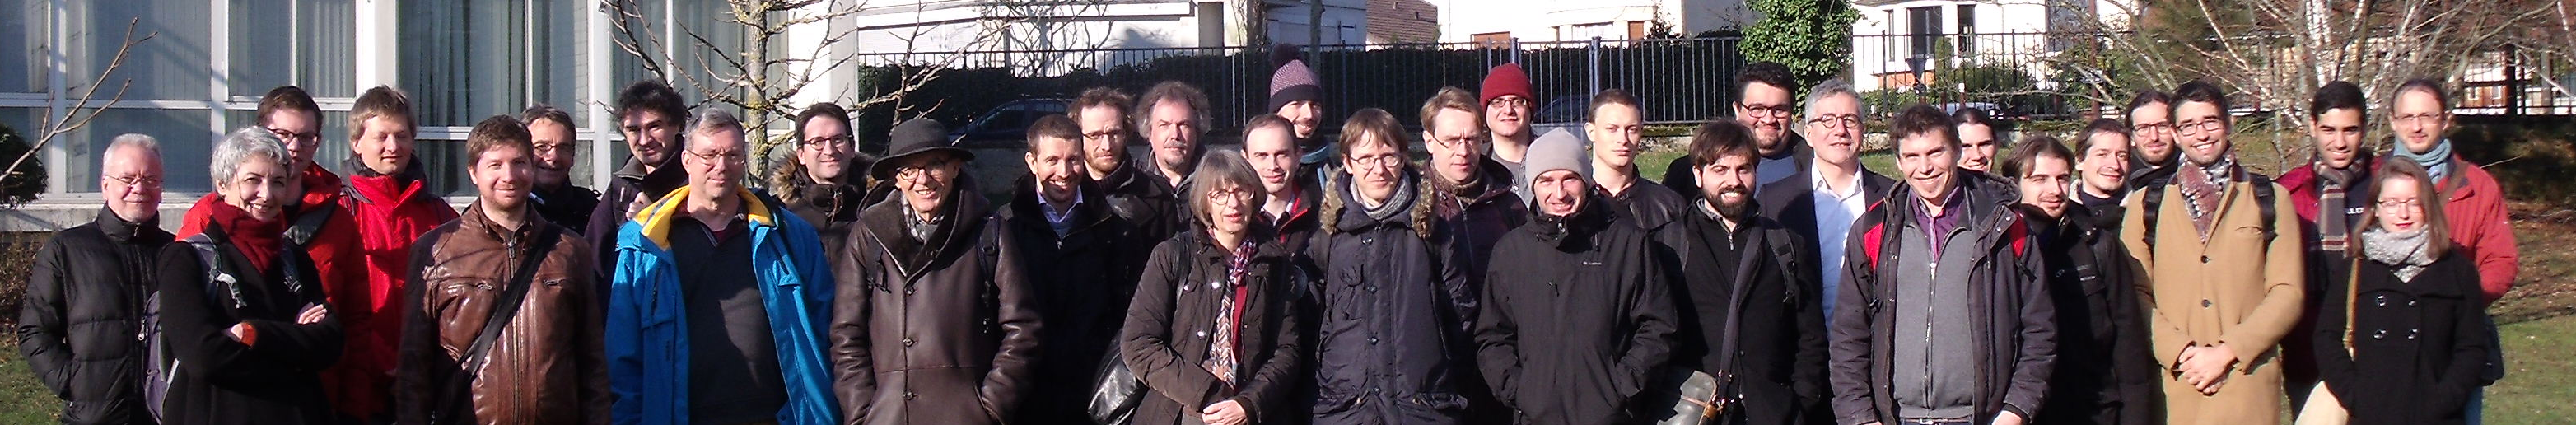
\includegraphics[height=2cm]{photo.png}
\end{center}
During this meeting, the idea of making this proof of concept a
European infrastructure emerged.  Since then, colleagues from Belgium,
Germany, Romania, Serbia, Sweden, and the United Kingdom, from
academia and industry, have expressed their interest in participating
in this effort.  These researchers and engineers are ready to
contribute to develop this encyclopedia, aiming at sharing proofs,
under a creative commons licence, making them searchable, accessible,
interoperable, and reusable.
\end{shaded}

%%%%%%%%%%%%%%%%%%%%%%%%%%%%%%%%%%%%%%%%%%%%%%%%%%%%%%%%%%%%%%%%%%%%%%%%%%%%%%
\begin{shaded}
\vspace*{-0.5cm}
\begin{center}
{\bf \Large How do proofs contribute to safety and security of software?}
\end{center}

Imagine the following casino game. At the beginning, a player is given
eleven euros. At each round, she throws a six-sided dice. If the
results is a six, then the game ends.  If it is a five, a four, a
three, or a two, she is given twice the amount of money she already
has. If it is a one she loses two euros, if she has at least two.
When the game ends, the player wins the money she got, except if she
has zero, in which case she loses one million euros.

This game can be modeled by the following programme:
\begin{center}
    \begin{minipage}{10cm}
\begin{verbatim}
n = 11
stay = True;
while stay:
    roll = random.randint(1,6)
    if roll == 6:
        stay = False
    else:
        if roll >= 2:
            n = n + 2 * n
        else:
            if (n >= 2):
                n = n - 2
print(n)
\end{verbatim}
    \end{minipage}
\end{center}

To be on the safe side, the player wants to be sure, before starting
playing, that she will never finish with zero.  And indeed, at all times
the content of the variable {\tt n} is an odd number,
thus it cannot be zero. {\bf This property ``nothing bad happens'' is
called the ``safety'' of this program.} This property is a
consequence of two simple theorems of arithmetic:
$$\forall x~(\mbox{\it odd}(x) \Rightarrow \mbox{\it odd}(x + 2 * x))$$
$$\forall x~(\mbox{\it odd}(x) \Rightarrow \mbox{\it odd}(x - 2))$$
meaning that, for all $x$, if $x$ is an odd number, then $x+2*x$ and $x-2$ are odd numbers too.
Hence, proving the safety of this programme amounts to prove these two
theorems.

Let's now consider the case where there is a tiny bug in the
program. For instance the {\tt 2} has been replaced by a {\tt 3} in
the instruction {\tt n = n + 2 * n}. The programme is then unsafe as
shown by the sequence $11, 9, 7, 5, 3, 1, 4, 2, 0$. Yet, testing this
program will, most likely, not reveal this bug, since it only
manifests very rarely.  In contrast, attempting to prove the
correctness of this program will reveal the bug as it is impossible to
prove the proposition
$$\forall x~(\mbox{\it odd}(x) \Rightarrow \mbox{\it odd}(x + 3 * x))$$
\end{shaded}

%%%%%%%%%%%%%%%%%%%%%%%%%%%%%%%%%%%%%%%%%%%%%%%%%%%%%%%%%%%%%%%%%%%%%%%%%%%%%%
%\begin{shaded}
%\vspace*{-0.5cm}
%\begin{center} {\bf \Large When mathematics are needed to verify the
%    correctness of a programme}
%\end{center}
%
%Prime numbers are used in a wide variety of applications:
%pseudo-random number generation, cryptographic algorithms, etc.  Thus,
%verifying the correctness of complex primality testing algorithms is
%critical.
%
%To do so, we need first to define primality, for instance
%
%$$prime(p) := 1<p \wedge (\forall n, (1<n\wedge n<p) \Rightarrow \neg(n\mid p))$$
%
%where $\wedge$ is the conjunction, $\Rightarrow$ is the implication,
%$\neg$ is the negation, and $n\mid p$ means that $n$ divides $p$.
%
%To lower the cost of primality testing, we use tests that are more
%efficient than the naive use of the definition.  For instance, a very
%simple improvement is to test the divisibility of the considered
%number, not by each of the smaller natural numbers, but only up to its
%square root.  Indeed, if a natural number $p$ can be factored into the
%product of two smaller natural numbers $m$ and $n$, one of them has to
%be smaller than or equal to the square root of $p$.  Therefore, one
%could give the following more complex, but more efficient, definition:
%
%$$prime'(p) := 1<p \wedge (\forall n, (1<n \wedge n*n\leq p) \Rightarrow \neg(n\mid p))$$
%
%To ensure that these definitions are equivalent one needs to prove
%the following statement:
%
%$$\forall p, prime'(p) \Leftrightarrow prime(p)$$
%
%It would have been easy to introduce a small bug
%in the new definition.  For example, one could have written
%$n*n < p$, instead of $n*n \leq p$.
%This would have resulted in accepting squares of primes as primes.
%
%Yet, attempting to prove the equivalence of these two definitions would
%have revealed the bug, as they cannot be proven to be equivalent.
%\end{shaded}

%%%%%%%%%%%%%%%%%%%%%%%%%%%%%%%%%%%%%%%%%%%%%%%%%%%%%%%%%%%%%%%%%%%%%%%%%%%%%%
\begin{shaded}
  \vspace*{-0.5cm}
  \begin{center}
    {\bf \Large What is a formal proof? What is a proof system?}
    \end{center}

Since Antiquity, we have known that
proofs, both purely mathematical ones, as in Euclid's elements or the
recent proof of the Kepler's conjecture by Thomas Hales, and proofs used
to establish the safety and security of software, can be built with a
limited number of rules, for example
\begin{itemize}
\item From $A\Rightarrow B$ (``$A$ implies $B$'') and $A$, deduce $B$.
\item From $A$, deduce $A\vee B$ (``$A$ or $B$'').
\item etc.
\end{itemize}
Yet for most of mathematical history, proofs have been written in
a pidgin of natural language and mathematical formulas. When proofs are
very long (as it is often the case for the proofs used in safety and security,
but also for some proofs in pure mathematics), mistakes are
very difficult to detect. For instance, dozens of wrong proofs of
the parallel postulate have been given through history, sometimes by the
best of mathematicians such as Ptolémée, Proclus, al-Haytam, Tacket,
Clairaut, Legendre, etc.

In the 1960s, Robin Milner and Nicolaas De Bruijn noticed that the
correctness of a mathematical proof could be checked by a
computer. This led to the development of the two first proof systems
in history: Milner's LCF and De Bruijn's Automath.

For instance, from the axioms
$$\forall x~(\mbox{\em philosopher}(x) \Rightarrow \mbox{\em human}(x))$$
$$\forall x~(\mbox{\em human}(x) \Rightarrow \mbox{\em mortal}(x))$$
we can deduce
$$\forall x~(\mbox{\em philosopher}(x) \Rightarrow \mbox{\em mortal}(x))$$
In the language implemented in Automath, this proof is written
$$\lambda x \lambda h~(g~x~(f~x~h))$$
\end{shaded}

%%%%%%%%%%%%%%%%%%%%%%%%%%%%%%%%%%%%%%%%%%%%%%%%%%%%%%%%%%%%%%%%%%%%%%%%%%%%%%
\begin{shaded}
\vspace*{-0.5cm}
  \begin{center}
{\bf \Large What is a theory?}
\end{center}

Deduction rules such as ``From $A \Rightarrow B$ and $A$, conclude
$B$'' are universal, but building proofs requires more rules, that are
often specific to a domain of knowledge and are called
``axioms''. Examples are the axioms of geometry, the axioms of
arithmetic, etc. These axioms constitute a theory.

At the beginning of the 20$^{\mbox{\footnotesize th}}$ century, an
axiomatic theory, {\em set theory}, has been proposed to express all
mathematical proofs. In the first half of the 20$^{\mbox{\footnotesize
    th}}$ century a few variants of set theory have been proposed, as
well as a few alternatives (such as \emph{Simple Type Theory}).  But
because these theories had not been designed for being implemented on
a computer, each proof system such as Coq, Isabelle/HOL, Mizar,
Atelier B, etc. implements its own theory.  {\bf Thus the rise of
computer-checked formal proofs has led to a multiplication of
alternative theories for mathematics.

This is the major obstacle to interoperability between proof systems.}
\end{shaded}

%%% Local Variables:
%%%   mode: latex
%%%   mode: flyspell
%%%   ispell-local-dictionary: "english"
%%% End:


\section{Objectives}
\begin{figure}
\begin{framed}
  \begin{itemize}
\item[LIL 1:]
The theory implemented in the system has been defined in
the lambda-Pi-calculus modulo theory and in Dedukti.

\item[LIL 2:]
The system has been instrumented so some of its proofs can be exported
and checked in Dedukti.

\item[LIL 3:]
A significant part of the library of the system has been exported and checked in
Dedukti.

\item[LIL 4:]
A tool has been defined to analyze the Dedukti proofs for the system,
detect those that can be expressed in a theory weaker than that of the
system, and translate those proofs into a weaker logic.

\item[LIL 5:]
Certain proofs of the system have been made available in Logipedia.

\item[LIL 6:]
All proofs of the system have been exported, translated,
and made available in Logipedia.
\end{itemize}
\caption{The Logipedia integration levels (LIL)\label{lil}}
\end{framed}
\end{figure}

To foster the interoperability of proof systems and the sustainability
and the cross-verification of formal proofs, we propose to collect
them in an online encyclopedia, called {\sf Logipedia}.  For each
proof, {\sf Logipedia} will indicate in which systems it can be used
and, when this is the case, it will provide a version of this proof in
the theory of these systems.

Such a project will not only foster the use of formal proofs in
research in mathematics and computer science, but also in industry, by
allowing cross-verification, sustainability, and interoperability of
formal proofs, and in education, freeing the teaching of formal proof
technology from being bound to one system.

Such a project can only have a worldwide ambition. However, as a
majority of proof systems are developed in Europe, there is a unique
opportunity for Europe to take the lead on such a project and prepare
the grounds for the economic spinoffs from the project benefiting
European industry. That is why the consortium gathers most of the
European actors active on formal proof systems, while also developing
links with non-European partners.

Building this encyclopedia is {\em per se} a networking activity
between the partners, from academia and industry, involved in the
project.  Currently, we know how to express the theories of {\sf HOL
  Light} \cite{Assaf12}, {\sf Matita} \cite{Assaf15}, {\sf Coq} and
{\sf FoCaliZe} \cite{Cauderlier16} in {\sf Dedukti} and recheck proofs
developed in these systems.  We aim at including, in twenty years, all
formal proofs developed at that time.
In the next four years, we plan to address the theories of {\sf
  Abella}, {\sf Agda}, {\sf Atelier B}, {\sf HOL4}, {\sf Isabelle},
{\sf Minlog}, {\sf Mizar}, {\sf SMT-Lib}, \tlaplus, {\sf Why3}, {\sf
  LFSC}, {\sf PVS}, and {\sf TSTP}.  Other systems, such as {\sf
  ACL2}, {\sf IMPS}, {\sf Lean}, {\sf Nuprl}, and {\sf Rodin}, are
kept for later, except if some other partners join the project (Figure
\ref{systems}). This effort will require, and contribute, to build a
network of research teams, much stronger than what we currently have.

Beyond our main focus on interactive systems, we also plan to
integrate some proofs coming from automated theorem provers, SMT
solvers, and model checkers, when these proofs have a manageable
size. We already have experience with Archsat \cite{Bury19}, iProver
\cite{Burel10}, and Zenon \cite{CauderlierHalmagrand15}. We plan to go
further in this direction, in cooperation with our colleagues working
on LFSC \cite{Stump09}. Thus beyond the teams focused on formal proofs, we
will extend this network to teams of neighbour communities, such as
the automated theorem proving community and the SAT/SMT community.

To measure the level of integration of an existing proof system and
associated proof library in {\sf Logipedia}, we introduce a metric:
{\em the {\sf Logipedia} integration levels} (Figure \ref{lil}) that
counts six levels.  Among the 17 systems we shall focus on we plan to
increase the {\sf Logipedia} integration levels of 10 of them to level
5 or 6.

The various systems addressed in the project are currently at those levels:

\begin{tabular}{ll}
Matita:& level 5\\
FoCaliZe:& level 3\\
HOL Light:& level 5\\
Coq:& level 2\\
Agda:& level 2\\
Atelier B:& level 2\\
Isabelle:& level 2\\
HOL4:& level 1\\
TSTP:& level 1\\
Minlog:& level 0\\
PVS:& level 0\\
Abella:& level 0\\
Mizar:& level 0\\
TLA+:& level 0\\
SMT-Lib:& level 0\\
Why3:& level 0\\
LFSC:& level 0\\

\end{tabular}

and we plan to increase these levels to 

\begin{tabular}{ll}
Matita:& from level 5 to level 6\\
HOL Light:& from level 3 to level 5\\
FoCaliZe:& from level 3 to level 5\\
Coq:& from level 2 to level 5\\
Agda:& from level 2 to level 3\\
Atelier B:& from level 2 to level 5\\
Isabelle:& from level 2 to level 5\\
HOL4:& from level 1 to level 5\\
TSTP:& from level 1 to level ???\\
Minlog:& from level 0 to level 3\\
PVS:& from level 0 to level 2\\
Abella:& from level 0 to level 2\\
Mizar:& from level 0 to level 3\\
TLA+:& from level 0 to level 2\\
SMT-Lib:& from level 0 to level ???\\
Why3:& from level 0 to level ???\\
LFSC:& from level 0 to level ???\\

\end{tabular}

This encyclopedia will be freely accessible through a web browser,
from any country in Europe and beyond. But an important effort will be
made to make this encyclopedia accessible to a large community of
specialists and non-specialists, but structuring the contents on
libraries, books, chapters, etc. Some of the libraries we start with
already have a structure (modules, qualified names, etc.) that it is
important to preserve.

We shall also develop ergonomic interfaces, search engines, etc. 


Finally, this project will trigger joint research activities between
its users and between its developers.  First, there are several
theories for which we do not have yet reached level 1, and for which
we need to understand how to express then in {\sf Dedukti}. Which is
an obvious joint research activity. Then, we need to define algorithms
to eliminate some axioms from proofs. Many such algorithms already
exist to eliminate the excluded middle, the axiom of choice, or the universes
from a given proof. We need to develop new ones, more specific to the theories
we address in this project.

In addition, each library contains definitions of natural numbers,
real numbers, etc. and, most importantly, logical connectors, that
must be aligned, that is structural results proved for one definition
of real numbers must be transported to any definition of an isomorphic
structure.

All these objectives contribute to building a new formal proof
community, focused on the values of knowledge exchange and
sustainability.

%%% Local Variables:
%%%   mode: latex
%%%   mode: flyspell
%%%   ispell-local-dictionary: "english"
%%% End:



\section{Relation to the work program}
\begin{todo}{from the proposal template}\color{red}
  This section must explain how the proposal addresses the specific challenge and scope of
  that topic, as set out in the work programme. Page 53-55 of the call.
\end{todo}
\begin{longtable}{|p{0.2\textwidth}|p{0.75\textwidth}|}
\hline
{\bf Research \newline e-infrastructures for formal proofs}
&
Proof systems and automated theorem provers are research
infrastructures. Each proof system comes with its own library, and
these libraries are also part of the research infrastructure.  Currently
these infrastructures are small, distributed and disconnected.\\
&
\hspace{0.4cm}
Logipedia aims at building a large, worldwide infrastructure from the
small ones by integrating them.  The integration effort is substantial
because the proofs in the various libraries are expressed in different
theories, and because key definitions are formalized in a different
way.  But this integration effort is doable and contributes to the
challenge of bringing to European researchers and engineers effective and
convenient access to the best research infrastructures, in order to
foster further advances in knowledge and technology.\\
&
\hspace{0.4cm}
This idea to structure a networking activity around the construction
and the use of an infrastructure is relatively new in computer science
and mathematics. Moreover Logipedia is not an infrastructure of
computers, like Grid'5000 is, but mostly an infrastructure made of
data and of algorithms manipulating these data.  As Logipedia is an
e-infratructure, its budget structure is different from a material
infrastructure. A small part of the resources is used for computers,
and a large part of the budget is used to develop networking
activities, trans-national, virtual and ergonomic access, and joint
research activities.\\
\hline
{\bf A starting commu-}
&
This project has never been supported under FP7 or Horizon 2020 calls.\\
{\bf nity} &
\hspace{0.4cm} It mobilizes twenty nine research groups (twenty one in
academia and eight in industry), which is
almost all the groups working on formal proof technology in Europe.
The success of the project requires such a large network.  Indeed,
just like, according to Metcalfe's law, the effect of a network is
proportional to the square of the number of connected users, we can
postulate that the effect of an infrastructure, like Logipedia, is
proportional to the product of the number of proofs it contains and
the number of its potential users, each of them being proportional to
the number of theories it supports. So, such a project needs a
critical mass to succeed. This is also why we have developed a corona
surrounding the project, constituted of four clubs of users: 
a club of industrial users, a club of academic users, a club of users in 
education and a club of users in publishing.
These clubs
already have some members, but they will develop during the four years
of the project, preparing the long term future of the infrastructure.
The members of the club of industrial users have written letters 
explaining their interest in the project, that are in the appendix of this
document. {\color{red} Do not forget to include the letters.}
\\
&
\hspace{0.4cm}
These groups are located in eleven European countries.  Some of these
countries have a large number of participants, some others fewer,
reflecting the diversity of maturity of the research on formal methods
in Europe. This project will contribute to develop the formal proof
culture in the European countries where it is still inceptive.\\
&
\hspace{0.4cm}
We should also point out the originality of this project within the
European strategy of Research infrastructure.\\
&\\
&
$\blacktriangleright$ A novelty of this project is that is
investigates how infrastructures can be used in mathematics and in
computer science.\\
&\\
&
$\blacktriangleright$ It investigates how immaterial infrastructure
can be used to structure a research community, just like material ones
do.\\
&\\
&
$\blacktriangleright$ It is focused on mathematical {\em a priori}
knowledge, while most infrastructures are focused on {\em a
  posteriori} knowledge, issued from measures, observations,
experiments, and field surveys.\\
&\\
&
$\blacktriangleright$ It also investigates how a common infrastructure
articulates the relation between research and industry.
\\
\hline
{\bf Compliance policy with EU regulations}
&
A data management plan will be provided according to Inria’s
compliance policy with EU regulations. We also engage ourselves to
make the evolution of the Logipedia e-infrastructure compliant
with the European charter for access to research infrastructures.\\

\hline
{\bf Networking activities, trans-national access, joint re-}
&
Three work packages described below are dedicated to networking activities
to collect the data that constitute the infrastructure: the formal proofs
that constitute Logipedia.
\\
{\bf search activities}
&
\hspace{0.4cm}
Logipedia will be publicly and freely accessible online through any
web browser and trough a package management tool, so trans-national
and virtual access are provided directly. Its administration will be
decentralized in various places in Europe with two mirror sites in
Saclay and in München. But we go beyond trans-national and virtual
access.  Two work packages described below are dedicated to improving
the quality of the access to the encyclopedia.\\
&
\hspace{0.4cm}
Finally, this project fosters new joint research activities. First,
between the members of the consortium. Then, between the members of
the consortium and other academic partners, in particular those
developing automated theorem proving systems. Next, between the
consortium and the industrial users of proof systems. Finally, between
the industrial users themselves, as using proofs developed by others
will foster joint developments. Two more work packages are dedicated
to these research activities.  Such joint research activities
currently exist in Europe to some extent.  Such a joint project is a
unique opportunity to strengthen the existing ones and create new
ones.
\\
\hline
{\bf Towards standardization}
&
This project will be a stepping stone for a possible standardization
of proof languages.
\\
&
\hspace{0.4cm}
Unlike other communities in computer science, the formal proof
community is somewhat skeptical with respect to standardization. And
indeed, it would not make sense to standardize a theory for proof
systems, just like it would make no sense to propose Euclidean
geometry as a standard all geometers should use.  Instead, such a
cooperative effort can lead to the standardization of a logical
framework, that is a language to express theories and proofs in any of
these theories. Proceeding slowly and in a cooperative thus may change
the attitude towards standardization in the formal proof community and
make a standardization process more widely accepted.
\\
\hline
{\bf Inter-disciplinarity}
&
This project includes mathematicians, logicians, and computer
scientists and therefore is clearly inter-disciplinary.\\
&
\hspace{0.4cm}
Yet, Logipedia is inter-disciplinary in an even more fundamental
way. Proving properties of a piece of software driving a car or
piloting an aircraft require to formalize part of the physical world
in which this piece of software evolves. In the same way proving
properties of simulation software, requires to formalize some
properties of the simulated object.  Thus, just like mathematics and
software are involved in any part of modern science, formal proof will
eventually spread, over time, in all areas of science.\\
&
\hspace{0.4cm}
One major obstacle to the formalization of, for example, simulations
is that they typically depend on large bodies of knowledge in
mathematics and physics.  Different proof systems may be better
suited for different applications, thus there is a natural tendency
for a diversity of proof formats, just like there is a natural
tendency for diversity in the use of programming languages.  Yet, when
it comes to formalizing a particular physical simulation, one needs to
have all the necessary knowledge accessible from a single infrastructure.\\
&
\hspace{0.4cm}
Formal proofs will eventually become pervasive, and
different disciplines may be tempted to use different systems.
Because inter-disciplinarity is required to formalize physical world
simulations, a unifying language such as Logipedia for exchanging
formal proofs between theorem provers is a must-have.\\
\hline
\end{longtable}


%%% Local Variables:
%%%   mode: latex
%%%   mode: flyspell
%%%   ispell-local-dictionary: "english"
%%% End:


\section{Concept and methodology}
{\bf \Large (a) Concept}

\begin{framed}
\begin{center}
{\bf \Large How do proofs contribute to safety and security of software?}
\end{center}
  
Imagine the following casino game. At the beginning, a player is given
eleven euros. At each round, she throws a dice. If the results is a
six, then game is over.  If it is a five, a four, a three, or a two,
she is given twice the amount of money she already has. If it is a one
she is taken two euros, if she has at least two.  When the game is
over, the player wins the money she got, except if she has zero, in
which case she looses one million.

This game can be modeled by program $p$
%import random 
\begin{verbatim}
n = 11
stay = True;
while stay: 
    roll = random.randint(1,6)
    if roll == 6:
        stay = False
    else:
        if roll >= 2:
            n = n + 2 * n
        else:
            if (n >= 2):
                n = n - 2
print(n)
\end{verbatim}

To be on the safe side, the player wants to be sure, before starting
playing, that she will never finish with zero.  And indeed, in all runs,
the content of the variable {\tt n} is always an odd number, thus it
cannot be zero. This property is a consequence of two simple
theorems of arithmetic
$$\forall x~(\mbox{\it odd}(x) \Rightarrow \mbox{\it odd}(x + 2 * x))$$
$$\forall x~(\mbox{\it odd}(x) \Rightarrow \mbox{\it odd}(x - 2))$$
%$$\forall x~(\mbox{\it odd}(x) \Rightarrow \mbox{\it odd}(x))$$
Hence, verifying the safety of this program, that is that the
proposition 
${\mbox{\it safe}}(p)$ holds, 
amounts to prove these three theorems of arithmetic.

A tiny bug in the program, for instance replacing the {\tt 2} by a
{\tt 3} in the the line {\tt n = n + 2 * n} makes the program unsafe
as shown by the sequence $11, 9, 7, 5, 3, 1, 4, 2, 0$. Yet, testing
this program will, most likely, not reveal this bug, that manifests
very rarely.  In contrast, attempting to prove the correctness of this
program will
reveal the bug as it is impossible to prove the proposition
$$\forall x~(\mbox{\it odd}(x) \Rightarrow \mbox{\it odd}(x + 3 * x))$$
\end{framed}
\pagebreak
\begin{framed}
  \begin{center}
    {\bf \Large What is a formal proof? What is a proof system?}
    \end{center}
        
Since Antiquity, we have known that
proofs, both purely mathematical ones, as in Euclid's elements or the
recent proof of the Kepler conjecture by Thomas Hales, and proofs used
to establish the safety and security of software, can be built with a
limited number of rules, for example
\begin{itemize}
\item From $A \Rightarrow B$ and $A$, deduce $B$.
\item From $A$, deduce $A~\mbox{\it or}~B$.
\item ...
\end{itemize}
Yet, through history, most mathematical proofs have been written in
pidgin of natural language and mathematical formulas. When proofs are
very long (as it is often of the proofs used in safety and security,
but also of some proofs in pure mathematics), mistakes in proofs are
very difficult to detect. For instance dozen of wrong proofs of
parallel postulate have been given through history, sometimes by the
best mathematicians such as Ptolémée, Proclus, al-Haytam, Tacket,
Clairaut, Legendre...

In the 1960s, Robin Milner and Nicolaas De Bruijn noticed that the
correctness of a mathematical proof could be checked by a
computer. This led to the development of the two first proof systems
in history: Milner's LCF or De Bruijn's Automath.  From
the axioms
$$\forall x~(\mbox{\em philosopher}(x) \Rightarrow \mbox{\em human}(x))$$
$$\forall x~(\mbox{\em human}(x) \Rightarrow \mbox{\em mortal}(x))$$
we can deduce
$$\forall x~(\mbox{\em philosopher}(x) \Rightarrow \mbox{\em mortal}(x))$$
In the language implemented in Automath, this proof is written
$$\lambda x \lambda h~(g~x~(f~x~h))$$
\end{framed}

\begin{framed}
\begin{center}
{\bf \Large What is a theory?}
\end{center}

Deduction rules such as ``From $A \Rightarrow B$ and $A$, conclude
$B$'' are universal, but building proofs require more rules, that are
often specific to a domain of knowledge and are called
``axiom''. Examples are the axioms of geometry, the axioms or
arithmetic. These axioms constitute a theory.

At the beginning of the 20th century an axiomatic theory, {\em set
  theory}, has been proposed to express all mathematical proofs. In
the first half of the 20th century a few variants of set theory, and a
few alternatives have been proposed (such as Simple type theory).
But, because these theories had not been designed for being
implemented on a computer, the rise of computer checked formal proofs
has led to a multiplication of such alternative theories. Each proof system,
such as Coq, Isabelle/HOL, Mizar, Atelier B,
etc. implements its own theory.

This is the major obstacle to interoperability.
\end{framed}

\bigskip

\noindent
{\bf \Large Logical Frameworks}

We had, in the past, an (informal) proof of Pythagoras’ theorem
or Fermat’s little theorem. The same proof now has different
formalizations in PVS, Isabelle/HOL, Coq, etc., jeoprardizing the
universality of logical truth.

In the 19th century, the universality of logical truth has been
jeopardized in a similar way, by non-Euclidean geometries, as some
statements could be true in one geometry, but false in others.  But,
at the beginning of the 20th century, a solution was found.  The
definition of the various geometries in predicate logic
\cite{HilbertAckermann} restored the universality of logical truth,
allowing to determine which axiom was used in which proof and which
theorem held in which geometry.

Predicate logic is not a theory in itself, but it is a framework in
which one can express theories, as sets of axioms: {\em a logical
  framework}.  Expressing the various geometries in predicate logic
allowed to analyze which proof contained which axiom, and hence which
proof could be expressed in which theory.

In 1928, predicate logic was a huge success, since three important
theories used at that time (geometry, arithmetic and set theory) could
be expressed in it. But it also has limitations, which explains that
another of the major theories used at that time (Russell's type
theory, from The Principia Mathematica) has not been expressed in
it. Since then, several other theories, such as Church's type theory
\cite{Church40}, Martin-L\"of's type Theory \cite{Martin-Lof84}, and
the Calculus of constructions \cite{CoquandHuet88}, have also been
defined as autonomous theories. These theories are those implemented
in most of the current proof systems, yet they cannot be expressed in
predicate logic.

This failure has led, in the field of proof systems, to the
abandonment of predicate logic, and even of the concept of logical
framework: the theories implemented in Coq, Matita, HOL Light,
etc. are often defined as autonomous systems, and not in a logical
framework.

However, a different line of research has attempted to understand the
limitations of predicate logic and to propose other logical frameworks
repairing them. The most prominent limitations of predicate logic are
the lack of function symbols binding variables, the lack of a syntax
for proof terms, the lack of a notion of computation, the lack of a
notion of cut for axiomatic theories, and the impossibility to express
constructive proofs. These limitations have led to the development of
logical frameworks such as $\lambda$-Prolog \cite{NadathurMiller88,
  MillerNadathur12}, Isabelle \cite{Paulson90}, the $\lambda
\Pi$-calculus (also called the ``Edinburgh logical framework'')
\cite{HarperHonsellPlotkin91}, Deduction modulo theory
\cite{DowekHardinKirchner03, DowekWerner03}, Pure Type Systems
\cite{Berardi88,Terlouw89}, and ecumenical logics
\cite{Prawitz15,Dowek15,PereiraRodriguez17}.

All these logical frameworks have been unified in the $\lambda
\Pi$-calculus modulo theory \cite{CousineauDowek07}, implemented in
the system Dedukti \cite{Assaf16}
on which Logipedia is based. Geometry, arithmetic and set
theory, but also Russell's type theory, Church's type theory,
Martin-L\"of's type theory, and the Calculus of constructions can be
expressed in this framework.

For instance, although the details are not important, Church's type
theory can be expressed in Dedukti , with 8 déclarations and 3
rewrite rules.
\begin{framed}
$\begin{array}{rcl}
type&:&Type\\
\eta&:&type \rightarrow Type\\
o&:&type\\
\mbox{\it nat}&:&type\\
\mbox{\it arrow}&:&type \rightarrow type \rightarrow type\\
\varepsilon&:&(\eta~o) \rightarrow Type\\
\Rightarrow&:&(\eta~o) \rightarrow (\eta~o) \rightarrow (\eta~o)\\
\forall&:&\Pi a:type~(((\eta~a) \rightarrow (\eta~o)) \rightarrow (\eta~o))\\
\\
(\eta~(\mbox{\it arrow}~x~y)) &\longrightarrow& (\eta~x) \rightarrow (\eta~y)\\
(\varepsilon~(\Rightarrow~x~y)) &\longrightarrow& (\varepsilon~x) \rightarrow (\
\varepsilon~y)\\
(\varepsilon~(\forall~x~y)) &\longrightarrow& \Pi z:(\eta~x)~(\varepsilon~(y~z))
\end{array}$
\end{framed}

So the theories implemented in various systems can all be expressed in
Dedukti and the proofs developed in these systems can be translated to
Dedukti. Just like in the case of non Euclidean geometry, this allows
to analyse the symbols and rewrite rules used in each proof
\cite{Thire18,Dowek17} (a domain traditionally called ``reverse
mathematics'' \cite{Friedman76,Simpson09}) and to deduce in which
systems each proof can be used.  This analysis is the basis of the
interoperability between proof systems.


\bigskip

\noindent
{\bf \Large The Logipedia integration levels}

\medskip

Thus, to make a formal proof, developed in some system $X$, accessible to
the users of other systems, the first step is to express the theory
$D[X]$, implemented in the system $X$, in the logical framework
  Dedukti.  Then, we must instrument the system $X$ so that the proof
can be exported from it, as a piece of data, expressed as a proof in
$D[X]$ and included in Logipedia. Next, we need to analyze this
proof in order to determine which symbols, axioms and rewrite rules of
$D[X]$ it actually uses and, thus, in which alternative theories it
can be expressed.  Finally, we must align its concepts with the
definitions already present in Logipedia and decide where it
fits in the general structure of the encyclopedia.

To measure the level of integration of an existing proof system and
associated proof library in Logipedia, we introduce a metric:
{\em the Logipedia integration levels} (Figure \ref{lil}) that
counts six levels.  

\begin{framed}
\begin{center}
{\bf The Logipedia integration levels (LIL)\label{lil}}
\end{center}

\begin{itemize}
\item[LIL 1:]
The theory implemented in the system has been defined in
the $\lambda\Pi$-calculus modulo theory and in Dedukti.

\item[LIL 2:]
The system has been instrumented so some of its proofs can be exported
and checked in Dedukti.

\item[LIL 3:] A significant part of the library of the system has been
  exported and checked in Dedukti.

\item[LIL 4:] A significant part of the library of the system have
  been made available in Logipedia.

\item[LIL 5:]
A tool has been defined to analyze the Dedukti proofs for the system,
detect those that can be expressed in a theory weaker than that of the
system, and translate those proofs into a weaker logic.

\item[LIL 6:]
All proofs of the system have been exported, translated,
and made available in Logipedia.
\end{itemize}
\end{framed}

The sixteen systems addressed in this project currently have different
integration levels, and we have different targeted levels for them.. 

\begin{center}
\begin{tabular}{|l|c|c|}
\hline
System & current level & targeted level\\
\hline
Matita & 5 & 6\\
\hline
HOL Light & 3 & 5\\
\hline
FoCaLiZe & 3 & 5\\
\hline
Coq & 3 & 5\\
\hline
Agda & 2 & 4\\
\hline
Atelier B & 1 & 5\\
\hline
ProB & 1 & 5\\
\hline
Isabelle & 2 & 5\\
\hline
HOL4 & 1 & 5\\
\hline
TSTP & 1 & {\color{red} ???}\\
\hline
Minlog & 0 & 4\\
\hline
PVS & 0 & 2\\
\hline
Abella & 0 & 2\\
\hline
Mizar & 0 & 4\\
\hline
Smart & 0 & 3\\
\hline
TLA+ & 0 & 2\\
\hline
 Why3 & 0 & {\color{red} ???}\\
\hline
LFSC & 0 & {\color{red} ???}\\
\hline
\end{tabular}
\end{center}

These systems can be roughly divided into two groups. Those in the
first half of the array (Matita, HOL Light, 
  FoCaLize, Coq, Agda, Atelier B, ProB, Isabelle,
HOL4, and TSTP) for which we have preliminary results and
that we plan to bring to a very high level of integration. Those in
the second half (Minlog, PVS, Abella, Mizar,
Smart, TLA+, SMT-Lib, Why3, and LFSC) with which we
are starting and for which our goal are less ambitious.

These two groups of systems will be addressed in different
work packages, but both are key to the project. The first ones will
constitute Logipedia in 2024 and the second ones prepare the
long term future of the infrastructure.

\bigskip

\noindent
{\bf \Large Instrumentation}

\medskip

Consider a system $X$ at LIL 1, so the basic theory $D[X]$ has
already been expressed in Dedukti. The next step is to implement a
method to automatically translate proofs from system $X$ to its
expression in Dedukti, and make these proofs available in Logipedia so
they can be exported to other systems. This step is called the
\emph{instrumentation} of system $X$.

The systems considered in this project fall into three broad classes:
\begin{description}

  \item[Systems based on dependent type theory.] Agda, Coq, and Matita
  are theorem provers based on Martin-L\"of's intuitionistic type
  theory.

  \begin{itemize}
    \item Coq is an interactive theorem prover developed at Inria
    since the 1984.  It is based on Type Theory and was used to
    formally verify the correctness of both industrially relevant
    software such as the CompCert C compiler and complex mathematical
    proofs such as the one of the Four Color theorem and the one of
    the Odd Order theorem. In 2013 Coq received the ACM system award.

    \item Matita is an interactive theorem prover developed at the
    University of Bologna and used for teaching logic courses and to
    verify software and mathematical proofs, with special attention to
    predicative foundations. The first generation of the system (up to
    version 0.5.9) was born as a by-product of the MoWGLI FET-Open
    Project, it was compatible with the logic of Coq and it could
    re-use its libraries. It was an important test-bench for the
    integration of Mathematical Knowledge Management techniques with
    Interactive Theorem Proving, featuring for example a library of
    theorems distributed over multiple servers, innovative indexing
    and search techniques and automatic translation of proofs between
    declarative and procedural styles. The second generation of the
    system (up to the current version 0.99.3) was a re-implementation
    from scratch that departed from the logic of Coq and that
    experimented with the most concise ways to implement an efficient
    theorem prover. Several ideas later migrated into Coq. The
    currently available largest library is the formal certification of
    a complexity-preserving and cost-model-inducing compiler from C to
    MCS-51 machine code, developed in the FET project CerCo (Certified
    Complexity).

    \item Agda is a dependently typed programming language and
    interactive proof assistant developed at Chalmers University of
    Technology as well as other places in Europe. The theory of Agda
    is similar to Coq and Matita, but is more focused on interactive
    development and direct manipulation of proof terms (in contrast to
    using a tactic language to generate the proof terms). To support
    the construction of proof terms, Agda provides powerful features
    such as dependent pattern and copattern matching, eta equality for
    functions and record types, first-class universe polymorphism, and
    definitional proof irrelevance. In addition, Agda provides an
    experimental option for extending the language with user-defined
    rewrite rules, which are very similar to the rewrite rules
    provided by Dedukti.
  \end{itemize}

  \item[Systems based on simple type theory.] (HOL4, Isabelle)
  \ednote{We still need some text to go here!}

  The HOL4 proof assistant is home to a few medium to large scale
  specifications and associated proof developments that have value
  outside of HOL4. These specifications include the formal semantics
  of the CakeML language (and its verified compiler) and an extensive
  specification of the ARM instruction set architecture (ISA) as
  formalised by Anthony Fox at the University of Cambridge.

  Isabelle as a logical framework \cite{paulson700} is an intermediate
  between Type-Theory provers (like Coq or Agda) and classic LCF-style
  systems (like HOL Light or HOL4).

\item[Systems based on set theory and first-order logic.] Atelier B,
  Rodin and ProB are platforms or tools to develop models written
  using the B method, a version of set theory expressed in predicate
  logic.  A model in these systems encodes a state machine constrained
  by invariant properties. Verification of the model correctness
  implies to verify some proof obligations produced by a weakest
  precondition calculus. For example, spanning trees algorithms,
  distributed algorithms, access control policies have been formalized
  respectivement in EventB and B method.

  The development process for the B method is based on formal proof:
  proof obligations are automatically generated and must be proven by
  automatic or interactive provers. This can include external solvers
  such as SMT solvers, and (in the case of ProB) constraint solvers
  such as Sicstus Prolog. The difference between Atelier B and Rodin
  lies mainly in the refinement process they implement: in the B
  method used by Atelier B refinement is done by deriving a program,
  while in Event-B used by Rodin refinement is done by defining a
  model of the system and iteratively introducing details. Finally,
  ProB is an animator and model checker: it helps users to gain
  confidence in their specifications, and it can be used as a
  disprover to discover counter-examples to proof obaligations.

  Smart is based on a classical first-order logic extended with rank-1
  polymorphism, algebraic datatypes, recursive definitions and
  inductive predicates. ProvenTools will turn models implemented in
  Smart to proof obligations which can be proved in the system using a
  mix of interactive and automated proving. The resulting proofs are
  reviewable objects, akin to proof traces built of the various atomic
  proof rules supported by ProvenTools' kernel, such as definition
  unfolding, case analysis or equality propagation.
\end{description}
Despite the large differences between these three classes of provers,
there are several common points between them where solutions that work
for one system can also be applied to other systems.
%
Concretely, we plan to tackle the following
research challenges:
\begin{description}

\item[Improving encodings.] Since Dedukti is designed to be a small
  logical framework with a minimal number of features, there are many
  features in the systems we consider that are not supported in
  Dedukti. Instead, such features need to be encoded in some way. In
  this work package, we consider systems for which it is known how to
  encode all features \emph{in theory}. However, depending on the
  choice of encoding, the instrumentation may be very hard or even
  unfeasible in practice. For example:
  \begin{itemize}

    \item Many Agda libraries (as well as some Coq libraries) rely
    heavily on type-directed conversion rules such as eta-equality for
    functions and record types, or definitional proof
    irrelevance. Dedukti does not provide type-directed conversion
    directly, so instead these rules have to be encoded by adding
    additional type information to the proof terms. This can hence
    lead to a large blow-up in the size of those proof terms, and thus
    greatly increase the cost of typechecking.

    \item Coq, Agda, and Matita all provide support for coinductive
    (infinite) structures, which are not supported natively in
    Dedukti. These structures can be encoded by rewrite rules in
    Dedukti, but this may cause the typechecker to go into an infinite
    loop.

    \item A few of the systems rely on AC rewriting (i.e.~rewriting
    modulo associativity and commutativity of certain operations), for
    example to encode universe polymorphism in dependent type
    theories. While Dedukti has support for AC rewriting, the current
    implementation is very slow, which makes typechecking the proofs
    in Dedukti unfeasible.

  \end{itemize}
  Finding better ways to encode such features could have a great
  impact on the quality and speed of the translation process.  We plan
  to investigate two possible approaches to improve the encodings of
  common features of proof assistants in Dedukti. First, we will
  investigate whether some information in the current encodings is
  redundant and can thus be omitted. Second, if this is not possible
  we will investigate what minimal changes need to be made to Dedukti
  itself in order to overcome these limitations.

  \item[Reconstructing transient proof components.] In all theorem
  provers, there is some information that is created during the
  process of checking a proof that is not stored in the final proof
  term. In systems such as Coq, Agda, and Matita, this concerns for
  example the types of each subexpression. In other systems such as
  HOL4, Isabelle, Atelier B, and Rodin, even more information about
  the proof is discarded and only the high-level proof steps remain.
  However, the translation from the system to Dedukti might rely on
  this transient information. Developing a method to reconstruct this
  transient information is thus crucial to the goals of this work
  package.

  In order to instrument systems with transient proof information, the
  proof terms need to be complemented with this transient information
  by either logging or re-synthesizing it on demand. Both approaches
  may be used, depending on the the tradeoff between computation time
  and space for storage.

  However, this approach is insufficent for systems that rely on
  external provers such as Isabelle or Event B. In order to handle
  these cases, we will instrument these external provers so they can
  produce the missing parts of the proof terms. 

  \item[Producing more compact proofs.] When translating a proof from
  some system $X$ to Dedukti, we want to produce proof terms that are
  as small as possible, so it is easy to store them, recheck them, or
  export them to a different system. However, there are at least two
  reasons why proof terms might become large. First, a typical proof
  in system $X$ might be very large (because big parts of it are
  constructed automatically). Second, translating a proof from $X$ to
  its encoding in Dedukti might greatly increase the size of the
  proof, for example by normalizing it or by adding type annotations.
  This means translating the proofs can take a very long time, and
  doing anything with the translated proof will be difficult. This
  also has an obvious impact on the exporting of complete libraries to
  Dedukti, which is the goal of WP3.

  To reduce the size of proof terms produced by the translation to
  Dedukti, we plan to investigate how to avoid unneccessary
  normalization or duplication of (parts of) proofs. We will also
  investigate what parts of each proof can be safely omitted because
  they can be inferred from the rest of the proof.
\end{description}

For each of the systems considered in this work package, we can
identify some preliminary work on translating proofs to Dedukti. Some
of these tools are in a preliminary stage and can only handle toy
examples, while others have been used to export whole libraries but
have not been updated to work with the latest version of the
system. Concretely, we plan to build upon the previous work done on
the following tools:
\begin{itemize}
\item The standard and arithmetic libraries of Matita has been the
  first libraries to be exported to Logipedia using Krajono, a fork of
  Matita. The forked system is also actually the only one able to
  import Logipedia proofs. The choice of Matita as a test-bench for
  Logipedia is easily understood considering that the implementation
  of the 0.99.x series was aimed at obtaining a well-documented,
  minimal but fast implementation of a theorem prover, two order of
  magnitudes smaller than Coq.  We plan to make this translation a
  part of the code of Matita itself so that it is maintained with the
  rest of the system.
\item CoqInE is a prototype tool that can translate Coq proofs to
  Dedukti. Recent work to include advanced features of Coq, such as
  universe polymorphism, has dramaticaly increased the coverage of
  this translation. We plan to make this translation a part of the
  code of Coq itself so that it is maintained with the rest of the
  system.
  \item In the summer of 2019, Guillaume Genestier worked together
  with Jesper Cockx on the implementation of an experimental
  translator from Agda to Dedukti during a research visit at Chalmers
  University in Sweden. This translator is still work in progress, but
  it is already able to translate 142 modules of the Agda standard
  library (about 25\%) to a form that can be checked in Dedukti. This
  exploratory work uncovered several challenges and opportunities for
  further work (see research challenges above).
  \item The inference kernel of Isabelle has already been instrumented
  to output proofs as $\lambda$-terms that can be understood by
  Dedukti. However, this has so far been only used for small examples
  \cite{Berghofer-Nipkow:2000:TPHOL}. The challenge is to make
  Isabelle proof terms work robustly for the basic libraries and
  reasonably big applications.  Preliminary work by Wenzel (2019) has
  demonstrated the feasibility for relatively small parts of
  Isabelle/HOL, but this requires scaling up.
  \item HOL4 has support for exporting proofs to the OpenTheory proof
  exchange format, and there has been some work on importing
  OpenTheory proofs into Dedukti.
  \item In the context of the BWare project, an encoding of the set
  theory of the B method has been provided as a theory modulo, i.e. a
  rewrite system rather than a set of axioms. This encoding is used by
  the automatic prover Zenon modulo which features a backend to
  Dedukti. Thus, as a first step through instrumentation of Atelier B
  and Rodin, proof obligations coming from Atelier B can be proved by
  Zenon modulo producing Dedukti proofs, hence providing a better
  confidence in the proofs produced by the native proof tools of
  Atelier B \cite{Bware}.
\end{itemize}

\bigskip
\noindent
{\bf \Large Automatic theorem provers: SAT/SMT solvers, first-order provers, etc.}

\medskip

We have discussed, in the last section, the instrumentation of proof
systems, that is interactive systems, where the users build formal
proofs with the help of the machine. Automatic Theorem Proving are
another type of systems, where the machine build proofs without any
human intervention. The proofs built by these systems are often
expressed in simpler theories than those developed using proof
systems, but they are not of a different nature. We will also include
in Logipedia proofs built by such automatic systems, whether they are
called automatic theorem provers, SAT solvers, SMT solvers, etc.

Several reasons explain the importance of these proofs for Logipedia.
{\em Per se}, many formal proofs nowadays rely on the use of automatic
provers. They cover various domains and various kinds of application,
{\em e.g.} combinatorial
mathematics~\cite{DBLP:journals/ai/KonevL15,DBLP:conf/sat/HeuleKM16},
where they are expected to solve one large propositional problem, or
proof of
programs~\cite{DBLP:conf/esop/FilliatreP13,DBLP:journals/pacmpl/ProtzenkoZRRWBD17},
where they are given thousands of small problems in a combination of
quantified theories.

In a complementary way, automatic theorem provers will be used to automatically make a
coherent whole out of Logipedia. A fruitful interaction between
formal proofs requires low-level glue which falls in the scope of automatic theorem provers.
For instance, they will be employed to fill the holes that appear when
considering provers with various granularity, to reduce the gaps between
proof systems, and to discharge proofs of concept alignment (in close
interaction with the work package 6).

Finally, automatic theorem provers will also benefit from
Logipedia. Obviously, Logipedia will be an extensive library of formal
statements that can be used and combined by automatic theorem provers
in their proof search. This is not trivial though: lemma selection is
crucial to avoid an overhead. It can also be a source of benchmarks to
evaluate their expressivity and automation.  Lastly, Logipedia and
Dedukti will form a framework to make automatic theorem provers
cooperate with each other and with other tools, in a safe way.

PF: TODO: Talk somewhere above about the various automatic theorem
proving tools, their specificity and why they are each of them useful
or would benefit from Logipedia

\medskip

\noindent
{\bf \large From automatic theorem provers to Dedukti}

Similarly to Interactive Theorem Provers, connecting ATPs to the Logipedia
infrastructure strongly relies on the ability for ATPs to import statements from
{\sf Dedukti} and export proofs in some theory in {\sf Dedukti}.

\begin{description}
\item[Instrumenting ATPs to produce proof traces.] The first step for connecting ATPs to the Logipedia infrastructure, and the library of proofs, is that ATPs should actually output some kind of proof, without enforcing strong requirement on the format or even the level of granularity of those proofs.  SAT (Satisfiability) solvers for propositional logic do have a perfectly well specified format for proof traces~\cite{TODO} and most SAT solvers are actually able to produce proof traces in that format.  So, considering SAT solvers, the current status is actually meeting the Logipedia needs on this aspect.

  Considering other automated reasoners however, it is mandatory to significantly improve the picture.  Some SMT (Satisifiability Modulo Theories) solvers do produce some kind of proof trace, but the format is specific to the solver, and the proofs are sometimes difficult to replay due to their granularity.  Most mainstream first-order theorem provers output proofs in a standardized language~\cite{TODO}, but this language does not clearly specify the semantics of the proof steps.  Model-checkers do not provide proof traces per se, although such traces would be useful for various usages and notably certification.

  Our goals are to improve reasoning tools to demonstrate the feasibility to
  produce sufficiently detailed proofs for connecting to Logipedia, and to
  design a set of theoretical methods and practical tools that can be used to
  further connect Logipedia to the other existing automated reasoners of the
  same kind.  We will work on three SMT solvers (alt-ergo, CVC4, veriT), two
  first-order provers (the E-prover, Zipperposition), and one model-checker
  (cubicle).  We will also consider more specific reasoning tools, with the aim
  to demonstrate that this approach also applies to more specific reasoners.  We
  envision to experiment the approach on a Coherent Logic reasoner.  These
  reasoners are particularly useful for geometry reasoning, and as such, they
  are quite complementary to the other considered automatic reasoners.  They are
  also very suitable as as a first experiment, since their proofs are fairly
  straightforward to interpret.  They thus constitute a very interesting low
  hanging fruit.
  
  It is not possible, and not even desirable, to require all tools to directly
  talk in the language of Logipedia.  Indeed, proof trace languages that are
  specific to one kind of reasoning tool are more appropriate than Dedukti for
  instrumenting already large pieces of software, enabling quick output, and
  allowing proof post-processing at the right level of abstraction on the
  produced proof traces.  Furthermore, provided that those proofs are detailed
  enough, translation of traces to Dedukti will not be a difficult task, and a
  the work necessary to translate proof traces for a myriad of very different
  reasoners will be implemented in a unique tool (Ekstrakto, see below) to take
  advantage of the fact that reasoning techniques, and thus proof methods, are
  themselves pretty shared among the solvers.

\item[Translate ATP traces into Dedukti] As pointed out above, it is easier to
  instrument provers to make them output traces instead of directly provide
  Dedukti proofs. The second step to connect ATPs to the Logipedia
  infrastructure is to reconstruct the proof traces in order to build Dedukti
  proofs from them. The proposed process is the following: each step of the
  trace is transformed into an independent subproblem; each of these subproblems
  is given to a prover that can output Dedukti proofs; proofs of the subproblems
  are then combined to produce a global proof of the original problem.  Since
  subproblems correspond to atomic steps of the proof trace, they are relatively
  simple, so that we are confident that the prover producing Dedukti proofs will
  not struggle to find a proof. This process is quite similar to what is done by
  the hammer tools of interactive theorem provers (Sledgehammer in Isabelle/HOL,
  HOLyHammer for HOL4, etc.) which reconstruct proofs from traces produced by
  automated theorem provers.

  This scheme has already been prototyped in a tool called
  \href{https://github.com/Deducteam/ekstrakto}{Ekstrakto}. Ekstrakto takes a
  TSTP file, as can be produced by e.g.\ the provers E and Zipperposition, and
  it uses Zenon Modulo and ArchSAT to prove the subproblems. Ekstrakto was
  designed to be agnostic w.r.t.\ the prover producing the trace; in particular
  it does not depend on the specific set of inference rules of the prover. It
  was also designed to be agnostic w.r.t.\ the prover used to prove the
  subproblems; it is only required that the prover can output a Dedukti proof in
  the correct encoding of first-order logic.

  Although Ekstrakto has already shown that it is a valuable approach, it is a
  work in progress. In particular, the following issues will be addressed in the
  project:

\begin{compactenum}
  % extension to other proof trace formats
\item Up to now, Ekstrakto can only understand traces in TSTP format as
  input. We plan to make it accept traces in other formats, notably traces
  from SMT solvers, as well as all formats that will appear when instrumenting
  other ATPs.

  % unprovable steps

\item  Some steps in the proof traces are not provable: their conclusion is
  not a logical consequence of their premises. However, they preserve
  provability: the original problem has a proof if and only if the
  problem with the conclusion of the step also has a proof. This is the
  case for instance of the Skolemization step in first-order automated
  theorem provers, of the introduction of new definitions, as well as
  the RAT property in traces produced by SAT solvers. The approach of
  Ekstrakto cannot be used here, because the subproblem corresponding to
  the step cannot be proved. However, since provability is preserved, it
  should be possible to transform a
  proof using the conclusion of the step into a proof using its
  premises. Such a transformation depends on the nature of the step that
  has been used. We plan to include in Ekstrakto a way to handle
  Skolemization and definition introduction, which are the two step
  families that are missing to be able to manage all traces from the
  major first-order theorem provers.

  % specialization for theories

\item  Dedukti-producing provers used by Ekstrakto, namely Zenon Modulo and
  ArchSAT, are meant for pure first-order logic. However, we would like
  to deal with proof traces that use some specialized theory,
  e.g.\ arithmetic or bit-vectors, as could be output by SMT
  solvers. Although such theories could be presented as a set of axioms
  in first-order logic, it is almost certain that neither Zenon Modulo
  nor ArchSAT could be able to find non-trivial proofs using these
  axioms. Here, the idea would be to develop small provers dedicated to
  a particular theory, and outputting Dedukti proofs. Such provers would
  be called when a step in the trace relies on said theory. These
  provers need not be very optimized, since trace steps are relatively
  small; this should help producing Dedukti traces. A way to achieve
  this could be to extend Zenon Modulo: indeed, Zenon modulo can find
  proofs modulo arithmetic, but it is not able to produce a Dedukti
  proof yet.

\end{compactenum}
  
\end{description}

\noindent
{\bf \large From Dedukti to automatic theorem provers}
%\label{concept:wp4:deduktitoatp}

In the other direction, Logipedia will constitute a source of
knowledge for automatic theorem provers. For this to be affordable, this workpackage will
study the following challenges.

\begin{description}
\item[Translate Dedukti statements into automatic theorem provers
  inputs] Automatic theorem provers are mostly based on (parts of)
  first-order logic.  Logipedia theorems, which mostly come from
  interactive provers, will be expressed in the Dedukti encodings of
  much more expressive logics, such as dependent type theory or simple
  type theory.  Theorem statements thus need to be encoded again to be
  manipulable by automatic theorem provers.

  Encodings from expressive logics to first order logic already exist,
  and are used for instance in {\em hammers} for using automatic theorem provers into
  interactive theorem
  provers~\cite{DBLP:conf/lpar/PaulsonB10,DBLP:journals/jar/CzajkaK18}.
  In these works, the encodings are specific to one system to be
  affordable. In Logipedia, we have to combine and take benefit
  from statements coming from the encodings of different systems based
  on different logics. The key challenge here are thus:
  \begin{itemize}
  \item to avoid the loss of meaning coming from a succession of
    encodings; and
  \item to encompass statements coming from different systems.
  \end{itemize}
  We plan to investigate a new approach where, instead of hammers, the
  encoding is a succession of fine-grained encodings dedicated to one
  aspect. These ``small'' encodings will offer the possibility to be
  activated independently depending on the origin of the statement. They
  give the other advantages of being modular, easily extensible, and
  more reliable: each encoding is simple, and may output proofs, {\em
    e.g.} using Ekstrakto. It will also crucially rely on the concept
  alignment provided by the workpackage 6.

  It is common in the automatic theorem proving community to evaluate the performance on
  sets of benchmarks. As a side effect of this task, a new set of
  benchmarks will be extracted from Logipedia to measure the
  performance of automatic theorem provers on problems coming from different logic, and from
  a combination of these logics. In our case, it will not only allow to
  compare automatic theorem provers but also to measure the success of this task by evaluated
  the quality of encodings, and comparing our ``small'' encodings by
  activating them or not.

\item[Logipedia as a source of knowledge for automatic theorem provers] Pascal

\end{description}


\noindent
{\bf \large Large scale application: formal verification of C code}

The use of formal methods in the industry requires to have approaches
that apply to a wide variety of cases. For the verification of C code,
the Frama-C platform features numerous techniques. One of them relies on
automatic solvers: Frama-C-WP. Since automatic theorem provers are built by making many
choices such as which heuristics or which algorithms to use, they
display blind spots where they are less efficient to solve some cases.
In order to overcome that, it is necessary to use the wide variety of
solvers which exist in a portfolio manner. The Why3 tool features the
ability to send problems to lots of provers in a uniform way. However
with so many tools written by different teams involved, the meaning of
the same concept in the different tools could be different. It would
lead to errors in the overall verification results. Moreover in order to
be applied more widely, formal methods must handle more concepts such as
floating points where their exact meaning is less clear that
mathematical integers. That leads to more opportunities for two tools to
interpret differently the same concept. Finally, an industrial user
sometimes needs to add some reasoning or simplifications for their
particular concept so that it is better handled by automatic solvers. It
is very easy to make an error in those simplifications.

In order to overcome these problems, we propose to gain insurances in
the interaction of these different tools and to speed the addition of
new features to handle new cases by using proof objects:
\begin{itemize}
\item Where the industrial user needs to define the concepts he wants to
  verify in its C code, we will add the possibility to import concepts
  from Logipedia. The user gain time by not having to define them
  himself and it ensures that we have proofs for the accompanying
  lemmas.
\item Where the simplification rules written for the industrial case are
  executed in Frama-C-WP, we will instrument it to generate Ekstrakto
  input in order to produce a proof of the correction of these
  simplifications.
\item Where the problems are transformed to fit the different provers in
  Why3, we will inspire from the fine-grained encodings (previous
  paragraph) to also generate Ekstrakto proof.
\item In the end, we will gather the Dedukti or Ekstrakto proof of the
  provers, the encodings, and the simplification rules, in order to
  assemble them in a coherent whole.
\end{itemize}
This part thus combines and validates most of the previous aspects of
this workpackage, but also constitutes the challenge to instrument a
large-scale formal tool.

\medskip

\noindent
{\bf \large Automatic theorem provers to increase Logipedia readiness}

\dots Chantal: T5 and T6

\subsubsection{Description of the work package 3}

\subsubsection{Description of the work package 7}

\subsubsection{Description of the work package 9}

\subsubsection{Description of the work package 2}

\subsubsection{Description of the work package 5 and 6}

{\color{red} Goals}

The development of formal reasoning tools has led to an ever-growing
corpus of mechanized mathematical theories. As these libraries span a
wide spectrum of proof assistants, the underlying logical foundations
of these systems and libraries can different greatly. For example,
some proof assistants use set theory as a foundation while others use
first-order logic, higher-order logic, or different variants of type
theory.  In order to combine the power of different proof assistants
and their respective communities, it is critically important that
these different logical foundations can be related to each other in
ways that ensure their interoperability.  Even when one has
successfully aligned these different logical foundations, one must
also align the many different mathematical concepts and theorems that
are in the libraries produced by the various proof assistants. Thus,
successful interoperability of both proof assistants and formalized
mathematical libraries starts with identifying the correspondences
between the concepts underpinning these formalizations, i.e., their
alignment.

In the simplest case, an alignment is a pair of symbol identifiers
from two different libraries such that both symbols are ``the same
informal mathematical concept''. For example, although real numbers
can be defined by Cauchy sequences, Dedekind cuts, and also stream
representations due to corecursion, all such different formalizations
introduce essentially the same mathematical concept. More precisely,
following the work of \site{Fau} and \site{Inn}
\cite{GKKMR:alignments:17} and the alignment-based mediator developed
by \site{Fau} in the OpenDreamKit project \cite{ODK:mitm:18}, we
consider an alignment to be a pair of
\begin{compactitem}
  \item $2$ identifiers $c,c’$ (usually from two different libraries
    $L,L’$), which are considered to represent the same mathematical
    concept
  \item additional data that governs how $L$-expressions using $c$ and
    $L’$-expressions using $c’$ correspond to each other.
\end{compactitem}
The source of alignments can vary and include manual collections
\cite{MRLR:alignments:17} and automatic, machine-learned collections
\cite{align_kaliszyk}.

Even when the various different proof assistants are all exporting their
proofs in Dedukti, the proper alignment of the theories underpinning
those systems is an essential task: for examples, simply taking the
union of all the different theories can create an inconsistent and,
therefore, useless combination.
%
Alignments can also be useful for joining formalizations done within a
single prover, since different formal libraries developed within a
single system can introduce different definitions of the same
mathematical concept (each more suitable to the library where it is
introduced).

To explain the need for concept alignment, we can compare this aspect
of the Logipedia project to the virtualization of computer operating
systems. In such virtualized systems, it is not sufficient for the
user to be able to run system A inside system B, she also needs to
have access to some device of the host system as device of the guest
system. For example, all operating systems have the concept of file
systems, keyboards, mice, etc, but they are all using technically
different definitions of these concepts.  For virtualization to
succeed, significant work is required to build bridges that formally
connect the different versions of these concepts.

The goals of this work package are first to understand the concept of
alignment, then to identify alignments across the various proof
assistants, and then to build tools to bridge these alignments. We
will develop standards, tools, and techniques that will allow concepts
to be aligned so that formal proof developments from one proof
assistant can be meaningfully used in other systems.

{\color{red} Content}

Concept alignment can happen at different levels:
\begin{itemize}
\item alignments of logical foundations,
\item alignments of theorem proving objects deals with aligning types,
  constants and theorems,
\item alignment of proofs deals with aligning tactics and
  inference rules that have similar effects on the state of proof
  development.
\end{itemize}
Within this work package, we will primarily focus on the alignment of
logics and theorem proving objects (the first two of these levels).

% The following is used instead of \paragraph in the alignment WP.
\newcommand{\parag}[1]{\medskip \noindent {\bf #1}} 
% To revert, uncomment the following line
%\newcommand{\parag}[1]{\paragraph{#1}}

\parag{Aligning logical foundations}
In order to align logical foundations we will develop novel ways of
relating theories represented in Dedukti, building on extensive
experience of the team in type theory, computer-assisted
formalisation, proof theory and reverse mathematics. We will
articulate our work according to the following key parameters for
distinguishing between theories: classical vs intuitionistic logic,
predicative vs impredicative definitions, treatments of equality, and
presence and absence of certain additional axioms, e.g., the axiom of
choice.

One of the major goals of this task will be the formulation and
representation in Dedukti of a core logical system that is both common
to all logical systems and supportive of modular analysis of its
extensions. We believe that such a logical system can be obtained as a
type-theoretic version of geometric logic, a certain well-behaved
fragment of first-order logic.  Such a treatment of geometric logic
will be of interest because we
believe that, over theories in such a logic, we can transform
classical proofs, using the law of excluded middle and the axiom of
choice, into constructive proofs.  This transformation will not also be
a theoretical result but also have practical value since we 
will seek to obtain feasible algorithms to
transform proofs based on classical principles to constructive proofs.
This effort will add a new dimension to a long-standing development of
proof theory that is still very much unexplored.

A further reason for the interest in this type theory is that it could
provide, with a sequence of extensions, a new setting for the
development of reverse mathematics in a type-theoretic setting. This
setting is in contrast to the standard reverse mathematics developed
in the context of second-order arithmetic. Again, the presence of
proof terms (encoded using Dedukti) adds a new dimension to a
well-established topic.

One consequence of this work is that it can make features of one
system available in other systems. For example, Minlog implements the
refined Dragalin-Friedman $A$-translation, so that classical proofs in
a certain class can be constructivised, which means that programs can
be extracted from such transformed proofs.  We would like to make this
feature of Minlog available to other proof assistants through Dedukti.
In order to carry it out, we will study both-directed encodings
between a subsystem of Dedukti and Minlog.

\parag{Aligning theorem proving objects (case studies)}
Since sets, functions, relations and numbers are ubiquitous in all
formalized mathematics, we will pay special attention to their
alignment. Additionally, geometry is a very interesting case study,
since it is traditionally introduced in many quite different ways
(both analytically, using various number fields, and synthetically,
using different axiom systems), and we shall pay special attention
to aligning different existing formalizations of geometry.

There are several ways to define numbers. For the natural numbers,
one can, for example, choose a definition based on Peano’s axioms which
relies on a unary representation of numbers which is suitable for
proving theorems. But for computing, a definition based on a binary
representation is better. For real numbers and functions, their
definitions often differ even between different libraries of the same
proof assistant.  Real numbers, for example, can be defined using 
Bishop style modulated Cauchy sequence, regular Cauchy sequence,
Dedekind cut, and stream representations using corecursion.
Similarly, geometry can be defined synthetically using Hilbert’s,
Euclid’s or Tarski’s axioms or analytically using coordinate systems and
algebra.  Therefore, our first step will be to import into Dedukti the
equivalence theorems between these different axiomatizations. In
practice we want to use a theorem $\Gamma \vdash_S T$ expressed in
system $S$ based on some axioms $\Gamma$ in a system $S’$ based on
different axioms $\Gamma'$ and different definitions.

\parag{Automated theory alignment}
Although alignments can be manually discovered and described, the
sheer size of existing formal libraries forces us to develop automated
support for finding and organizing alignments.


We propose a workflow based on database and semantic web
methodologies. Specifically, we aim to build an automatic alignment
engine on top of an ontology framework that defines mappings between
base concepts belonging to different theories. Relying on a graph of
dependencies that indicates how the theories are structured within a
given library, we set to propagate the alignments with the help of a
certified matching-based engine. The engine will provide a way of
inferring new alignments, based on the alignment of the primitive
concepts and on a set of rules that will describe further
derivations. In order to enable flexible alignments, we are prepared to allow
not only exact matchings, but also matchings with respect to a given
similarity measure, as in \cite{???}.

An alternative method for discovering ontologies of alignments is
to use unsupervised learning methods to find alignments between proof
assistant repositories. For this, heuristic algorithms and dynamic
processes have been tried in the past \cite{???}.  As part of the
project we intend to also try to use unsupervised machine translation
algorithms \cite{???} to directly find correspondences between
statements and their constituent constants and types in proof
assistant libraries imported in Logipedia.

\parag{Alignment based services}
This task is concerned with the implementation of useful services
enabled by the discovered alignments. Each service implemented on top
of Dedukti---such as accessing a library via browsing or searching
or interoperability and reuse provided by translations across
libraries---will benefit from working up-to-alignments. For example, a
user of system $L$ can go to Logipedia to find a theorem about $t’$
about concept $c’$, defined in $L’$ that is missing in the library of
$L$. Even if $L$ contains the corresponding concept $c$, because $t’$
is stated and proved in the logic of $L’$, it will use a
different definition of $c’$ in $L’$ than the one of $c$ in $L$.
Therefore, $t’$ cannot be directly used in $L$. By translating $t’$
along the alignment $(c,c’)$, it induces a theorem $t$ that can be
used in $L$. The details are subtle both in theory and in practice,
and this task will explore how to scale up the alignments found in
\taskref{alignment}{alignlogic}-\taskref{alignment}{aligntheories} to
provide strong services.

This task will leverage this simple idea in multiple different
ways. Firstly, we will use alignments to search across libraries. In
its simplest form, this involves a simple search interface into which
the user enters the term $t$ and the system finds $t’$ because it uses
the alignment $(c,c’)$. Secondly, we will develop translation services
that use alignments to port proofs across libraries. This translation
will allow porting the proof of $t’$ in $L’$ to a (potential) proof of
$t$ in $L$.

% DM continue here

{\color{red} PROBLEMS}

Often there are many notions that are tightly connected, but not
equivalent. For example, some definitions are only special cases of
the others, sometimes there are definitions valid in any dimension and
some that are valid only in some dimension, sometimes definitions
differ only in the treatment of some corner cases (e.g., Hilbert's
axioms of geometry use strict betweenness, but Tarski's axioms use
non-strict betweenness relation). Although such alignments are also
needed, they are very hard to detect and use. An automatic prover
would fail because the two concepts are not equivalent, but they are
related in the sense that equivalent up to some special cases. Some
equivalences are highly non-trivial but for some others we can expect
to prove them automatically.

{\color{red} CONTRIBUTION TO NETWORKING, ACCESS AND RESEARCH}

Concept alignment between such a large body of formal libraries and
tools has never been attempted before, so it requires a joint research
activity of a large number of researchers all around Europe. Alignment
based services developed within this work package will significantly
facilitate access to the available body of formalized mathematical and
computer science knowledge.

{\color{red} RELATION TO THE OTHER WORK PACKAGES}

For geometry, we will rely on the \taskref{libraries}{geocoq}
(GeoCoq), and for constructive analysis, we will rely on
\taskref{theories}{minlog}. We envisage a collaboration with
\WPref{structuring}, aimed at reusing the ontology framework
integrated in the core of Dedukti. We also plan to collaborate with
\WPref{atpetc} on developing a case study regarding ATP proof
obligation discharge modulo alignment. It will be crucial to make
automatic theorem provers benefit from Logipedia as a library.

{\color{red} THE WAY TO KNOW YOU HAVE SUCCEEDED }

The final product of this workpackage are alignment aware services
that enable searching and browsing modulo alignment, and also enable
automated translation of theorem proving objects and proofs. However,
before such an ambitious goal could be achieved, many lessons must be
learned and several milestones must be achieved.
\begin{itemize}
\item A very precise definition of alignments should be given and a
  format (and an ontology) for describing and organizing alignments
  must be described.
\item Proof theoretical results relating different logical foundations
  must be obtained and an efficient algorithm for translating
  statements from one logical system to another must be implemented.
\item Alignment of basic mathematical objects (sets, functions,
  relations, numbers) must be ensured.
\item A method for automated detection of alignments must be devised,
  implemented and applied on a large corpus of formal libraries.
\item A case study of geometry must show that it is possible to align
  large formal theories developed in different theorem provers, based
  on different approaches (synthetic vs analytic).
\end{itemize}

{\bf (b) Methodology}

The methodology is the same for integrating any library to Logipedia,
but due to a difference of readiness of the various systems we focus on,
our priorities are different.

\begin{enumerate}
\item We already know how to express most of the theories of Atelier B,
Coq, FoCaLiZe, HOL Light, HOL4, 
Isabelle, Matita, and Rodin in  Dedukti. We propose
to instrument these systems so that they can produce Dedukti
proofs that we can include in Logipedia.

\item For other theories, such as those of Abella, Agda, Lean, Minlog,
  Mizar, PVS, TLA+, the work is in progress, or not yet started.  So
  we must first understand how they can be expressed in Dedukti.

\item Besides the standard libraries of these systems, large libraries
  have been developed: the Isabelle Archive of formal Proofs \cite{AFP},
   Flyspeck \cite{Flyspeck}, MathComp\cite{Mathcomp}, 
  CompCert \cite{Compcert},  CakeML \cite{CakeML}, ...  We aim to include
  some of these libraries in Logipedia.
  
\item
Besides proof systems, we also want to include proofs coming from
automated theorem provers, SAT solvers, SMT solvers, and model
checkers.  So we must instrument some of these systems so that they
can produce Dedukti proofs that we can include in Logipedia.

\item
We want to develop algorithms to analyze which symbol, axiom, rewrite
rule is used in each proof, and consequently in which system each proof
can be used. We also want to develop algorithms to eliminate some of the 
symbols, axioms, and rewrite rules used in a proof in order to be able to 
use it in more systems.


\item
Each library imported in Logipedia will come with its own
definition of natural numbers, real numbers, etc. We want to develop
``concept alignments algorithms'' to transport theorems from one
structure to another isomorphic one.

\item 
Besides data, we propose to include in Logipedia, metadata and
an inner structure.
\end{enumerate}

\subsubsection{Methodology of work package 1: instrumentation}

We know how to express in Dedukti the theories implemented in Matita,
HOL4, Coq, Agda, Isabelle and Atelier B, and some of these systems
have been partially instrumented to export proofs that can be checked
in Dedukti. Our first work package is to complete this instrumentation
to be able to export most of the proofs of these systems. As a
consequence, the work includes a strong practical component.

Three methods have to be used here: some of the systems (Automath
style), such as Coq and Agda already have proof-terms that can be
output, thus the main task is to translate these proofs into the
Dedukti format. Others (LCF style), such as Isabelle and HOL4, have an
inference kernel that can be instrumented, the main task here is to
transform the internal proof-object into an external
proof-term. Others, such as Atelier B are slightly more difficult to
address. For those, we need to use the water ford method: extract an
incomplete trace (a sequence of lemmas) and fill the gap using
automated theorem proving, as experimented with Atelier B and Zenon.

% A technological hurdle in the instrumentation of the systems under
% consideration is that all of them are actively developed systems
% that are constantly evolving.

\subsubsection{Methodology of the work package 4}

\subsubsection{Methodology of the work package 3}

\subsubsection{Methodology of the work package 7}

\subsubsection{Methodology of the work package 9}

\subsubsection{Methodology of the work package 2}

\subsubsection{Methodology of the work package 5 + 6}

\paragraph{Aligning logical foundations}

Our first step will be to divide logical theories in clusters,
according to the key parameters mentioned above, and then to build a
web of syntactic translations between systems. We do not expect full
back-and-forth translations, as some systems are well-known to be
proof-theoretically stronger than others, but we will seek to
establish suitable equiprovability results for fragments of the
relevant languages.

We shall also deal with specific case studies to test our work.  For
example, to test our methods for translating classical proofs into
constructive ones, one could verify Michael Beeson's "wholesale
importation" (he uses the double negation translation to import all
the negative results from \cite{} to intuitionistic logic) using the
library of GeoCoq proofs.

\paragraph{Aligning theorem proving objects (case studies)}

We call big scale concept alignment the equivalence between different
axiom systems, and small scale concept alignment the equivalence (or
relationship) between different definitions.  Big scale concept
alignment is the alignment of different theories, usually expressed
using different axiom systems (eg., Tarski, Hilbert, Euclid) for
different geometries: euclidean and non euclidean. It also includes
alignment of different kind of analytic definitions of geometry i.e.,
between different analytic models (e.g., real closed fields, reals,
complex numbers), different definitions of projective
geometry. Porting GeoCoq to other proof assistant will bring some of
these big scale concept alignments.  Small scale concept alignment
requires proof of equivalence between different definitions of the
same concept in the same or different language.  To some extent this
task could be automated, but the difficulty is that some equivalences
are valid only in some contexts.

\paragraph{Automated theory alignment}

In one line of research, we set to use logic-deduction approaches that
have been developed for the automatic alignment of database schemas
and instances, such as \cite{}.  In order to align theories across
libraries, we will propagate alignment information, based on a
certified probabilistic inference engine, which will extend the work
in \cite{}. We envisage a collaboration with WP7, aimed at reusing the
ontology framework integrated in the core of Dedukti. Concretely, each
of the domain-specific meta-data, essentially the theory schemas, will
be specified in the ontology framework. Their validity with respect to
the underlying instances will be mechanically checked and the
alignment of the schemas will inform that of the underlying theories.

In the second line of research, we will employ machine learning
techniques, based on neural networks, to design heuristics for finding
new alignments.

\paragraph{Alignment based services}

\textbf{Expression Translation.}

\textbf{Search Service.}

\textbf{Proof Rewriting.} In the recent literature there are two main
approaches to alignment based proof rewriting. The first one, based on
logical relations, has been proposed to translate a proof about $X$
into a proof about $X'$ remaining in the same logic. A relation is
established between elements of $X$ and elements of $X'$ where, for
example, $X$ can be the type of sorted lists of numbers, $X'$ the type
of balanced search trees and the relation holds between data
structures that contain the same set of integers. Then,
oversimplifying, for each pair of corresponding functions acting
respectively on $X$, $X'$, it is shown that they map related elements
to related elements. Continuing the example, the function that inserts
a new integer into the sorted list and the one that does the same into
the balanced search tree map data structures that contain the same
elements to data structures with the same property. Such proofs can be
obtained fully automatically when the functions are obtained
compositionally, without operating directly on the data structures. In
the remaining cases a human needs to provide the proof.

The first methodology is very accurate, but it requires human
intervention and it can be applied only when the alignments can be
simply expressed as relations between types and when everything is in
just one logic. The second methodology is less accurate, but somehow
more practical: it converts a proof into a sequence of intermediate
statements that need to hold, it translates each statement from one
system to the other ignoring the justification for the statement and
it fires an automated prover to fill the gap in the target system. By
varying the level of granularity the automated provers are allowed to
find alternative proofs, for example when some low-level properties of
data structure $X'$ are not available on data structure $X$, but a
different proof can still establish a statement that does not involve
them. Even when the provers fail to fill the gap the proof sketch
obtained can still be useful to the user that can try to manually fill
the gaps instead of restarting from scratch.

The task requires implementing multiple transformations and
translations of expressions containing binders (statements, proof
terms, etc.), which is well known to be a delicate task. ELPI,
developed by a join Ubo-Inr team, is a very high level programming
language of the logic programming family that allows to concisely
manipulate expressions with binders eliminating the most frequent
sources of mistakes (name capture, for example). ELPI comes with an
interpreter implemented in Ocaml that has been designed to be easily
integrated in other Ocaml based tools, like Coq. We plan to first
integrate ELPI in Dedukti so that Dedukti/Logipedia expressions can be
directly manipulated into ELPI. We also plan to implement means to
call external provers from ELPI via Logipedia translations. Then we
will use a mix of ELPI code and Dedukti rewrite rules to implement
alignment based proof and statement rewriting. Statement rewriting
will find direct application to alignment based search and browsing as
well.


\subsection{Readiness of the project}

This idea of building such a standard for proofs has already been
investigated in the past, such as in the Qed manifesto \cite{Qed94}, but
has produced limited results.

Our thesis is that, since the
Qed project, the situation has radically changed. After
thirty years of research, we have an empirical evidence that most of
the formal proofs developed in one of these systems can also be
developed in another. We understand the relationship between the
theories implemented in these systems much better. We have developed
several logical frameworks, extending predicate logic, in which these
theories can be expressed. And we have developed reverse mathematics
algorithms to analyze which axioms and rules are used in each proofs
and algorithms, such as constructivization algorithms, to translate
proofs from one theory to another.


%%% Local Variables:
%%%   mode: latex
%%%   ispell-local-dictionary: "english"
%%% TeX-master: "propB"
%%% End:


\section{Ambition}
\begin{todo}{from the proposal template}\color{red}
  This section must explain how the proposal addresses the specific ambitions (i), (ii),
  and (iii) on page 54 of the call, that are described in more details in appendix D. page
  107 of the call.
\end{todo}
\subsection*{Progress beyond state of the art}


\begin{longtable}{|p{0.2\textwidth}|p{0.75\textwidth}|}
\hline
{\bf Networking activities}
&
This project will include several types of networking activities, to
foster a culture of cooperation between scientific communities, that
are today often too centered around one system and one theory.\\
&
\hspace{0.4cm} First, the development of a common infrastructure is
\emph{per se} a networking activity, as the twenty nine partners of the
project have to join their forces towards a common goal (which is much
more an integrating activity than, for instance, organizing a common
conference). Then as the partners will also use this infrastructure
for their own developments, they will have to understand what the
other partners are doing, and how this can help in their own work.\\ &
\hspace{0.4cm}
This effort will also help to develop the formal proof community in
countries where it is still at an early stage of development.\\
&
\hspace{0.4cm}
This will also strengthen a culture of cooperation between scientific
researchers and engineers in academia and in industry. Currently this
cooperation is too often point to point (for instance a company uses a
one system and develops links this the group of academic researchers
developing this system). But we need to develop a more comprehensive
culture of cooperation, around common languages and a common research
infrastructure.\\
&
\hspace{0.4cm}
Our action in this direction is twofold. First, some companies that
already have a strong commitment in formal methods (Clearsy, CEA,
MED-EL, etc.) are included in the project as partners. May be, more
importantly, other companies, that could not be part of the project
because the project is too small, or that have a less developed
culture in formal methods are members of the ``club of industrial
users''. This club, among other goals, participates to develop a
culture of technology watch in formal methods in industry, which is a
stepping stone for developing a strong industrial awareness in safety
and security in European industry. This club also is currently too
small, but we are confident that organizing this club will only be a
first step, that will be followed by others.\\
&
\hspace{0.4cm}
It is important to develop a similar culture of technology watch for
researchers who are outside, or at the border of formal methods.  This
is why we have also organized a ``club of academic users'' that
gathers colleagues from our community that could not participate to
this project and colleagues outside the formal methods community, in
particular working mathematicians who are understanding the long term
impact formal proofs will have on mathematics.\\
&
\hspace{0.4cm}
It is also important to develop a similar culture of technology watch
for teachers, including high school teachers who are investigating how
a library of formal proofs can be used with younger students.  This is
why we have also organized a ``club of users in education''.  Here we
do not advocate teaching formal proofs to pre-schoolers (we should not
repeat the mistakes of the past), but we claim that having rigorous
statements of theorems in high-school textbooks (including all the
corner cases that are often omitted) and a clear dependency of which
theorem is used in the proof of which is a way to foster a culture of
rigor in high-school teaching, which is both useful for the students
who will take science at University and to those who will not. In
particular, we want, in this way, to contribute modestly to the
renewal of the culture of logical thinking, which is of prime
importance in our ``post-truth era''.\\
&
\hspace{0.4cm}
We also believe that an early exposition to formal statements and / or
formal proofs may contribute to compensate the shameful gender balance
in our research community. Here also, we must remain modest, as
achieving a decent gender-balance will require more than a single
action, but is is obviously much more effective to try to promote
contemporary scientific ideas, and encourage scientific carriers, to
women at the high school level rather that at the university level,
because at the university level there are already very few women in
our auditoriums.\\
&
\hspace{0.4cm}
We also plan to develop networking activities with publishers
(Elsevier, Springer, etc. but also, ArXiv, HAL, Wikipedia, etc.)  in
such a way that formal proofs mentioned in research papers and in
other encyclopedia can be made accessible, in Logipedia, for a long
period ot time, while currently, they are often just made accessible
on the web page of the authors.\\
&
\hspace{0.4cm}
These four clubs of users in industry, research, education, and
publishing, together with the partners of the project, will also
prepare a larger community that will develop Logipedia beyond the end
of the project, so that Logipedia contains all the formal proofs then
developed in twenty years.\\
&
\hspace{0.4cm}
Finally, Logipedia also prepares another kind of networking activities
beyond the duration of the project, as this effort will eventually
lead to the discussion of standards for proof languages.\\
&
\hspace{0.4cm}
We, of course, plan to organize the usual networking activities,
such as a yearly conferences with associated workshops on applications
in industry, research, education and publishing, a general assembly
where the research directions can be discussed collectively. And
summer schools, specially at the beginning of the project in order to
train the new participants (doctoral students, post-docs, etc.) to the
technology developed in Dedukti and Logipedia.
(See Section Dissemination and Communication.)\\  
\hline
{\bf Trans-national access and virtual access}
&
Logipedia will be accessible online. It will therefore be accessible
at no cost, and without identification, from every country in Europe
and beyond, just like, for instance, Wikipedia is.\\
&
\hspace{0.4cm}
The licence chosen for the Logipedia proofs needs not be the same for
all proofs, because some proofs already have a licence before being
imported in Logipedia and, in some cases, this licence must be
preserved.  Yet, in general we will favor a creative common licence
and in particular cc-by.  Such a licence allows a free
access, a findable, accessible, interoperable, and reusable
data management. It will contribute to the development of the Open
data / Open science / Open innovation philosophy.\\
&
\hspace{0.4cm}
Being a central infrastructure, Logipedia will contribute to abolish
internal European borders as, today, researchers and engineers often
use a system developed in their own country (only a few systems having
an international community of users), and libraries of formal proofs
specific to this system.\\
&
\hspace{0.4cm}
As explained above, our effort on access goes beyond providing a
trans-national and virtual access, as accessibility depends also on
developing an ergonomic web interface, a package distribution system,
a search engine, and an ontology of mathematical concepts. The public
targeted by these interfaces also has to be taken into account, a
secondary school student looking for a theorem in geometry needs a
different interface from a engineer looking for the correctness proof
of an algorithm.\\
\hline
{\bf Joint research activities}
&
The project includes two types of joint research activities.  First,
as any infrastructure, it will allow joint research projects between
the users of this infrastructure that will be able to develop new
proofs together using different systems.\\
&
\hspace{0.4cm}
Second, as any infrastructure, Logipedia raises new research
problems. Some of them have already been solved in the past and
require to be implemented jointly. Others are newer.\\
&
\hspace{0.4cm}
First, as we have explained, using a common infrastructure, requires
to describe the theories implemented in the different systems in a
common logical framework. We have already discussed how the expression
of geometry, arithmetic, and set theory in predicate logic has
permitted a renewal of logic at the end of the 1920's, allowing all
the logicians to speak the same language, and we can expect a similar
renewal here, fostering new joint research through the sharing, not
only of a common infrastructure, but also of a common language.\\
&
\hspace{0.4cm}
The development of a common encyclopedia, such as Logipedia, also
raises completely new problems such as automatic concept alignment,
structuring a large body of knowledge, or the development of
interfaces. These problems will trigger new cooperation between the
partners of the project and beyond.\\
\hline
\end{longtable}

\subsection*{Innovation potential}

Formal methods are at a turning point. Several academic and
industrial successes have proved the readiness of the technology,
in particular in critical systems where it has helped in
dramatically improving the quality of the systems. But this
technology takes too much time to be adopted in a broader context.

Limiting factors, probably the main ones, are the redundancy of the
efforts to develop proof systems, the lack of a common theory or at
least a common language to express the various theories, the lack of
common benchmarks, and the lack of standards for these systems.  For
industry, at least three key aspects slow down the adoption of formal
methods.

First, reusing a proof produced with a particular tool in another
can only be done at a high cost, when it is even possible.
Logipedia will help reducing this cost by unifying tools
around a common format, enabling the possibility to share proofs
between tools. In the uncommon case where a proof relies on a theory
which is not compatible with the target tool, it will be easier to
understand why and determine whether adapting it is managable.
Furthermore, as an infrastucture, Logipedia will help users
in finding existing proofs of properties, making their verification
process faster.

Second, checking a proof must remain possible over time. Today, it
requires either to maintain proofs along new versions of the tools,
which can represents a significant maintenance cost, or to archive
them together with a version of the tool used to produce it. In this
situation, Logipedia will help on two aspects. First, the
common format will guarantee that proofs can be checked by any tool
implementing it, thus reducing proof maintenance cost. Second, by
providing a common proof database, general interest proofs can be
stored and maintained in the infrastructure, allowing industrial users
to focus their resources for their specific needs only.

Finally, a proof or verification tool can be mistrusted. For example,
in a certification context, the use of a particular tool for the
verification of the candidate system must be approved. If the
certification body is not familiar with the tool, producing a
justification for it can represent a significant amount of time. For
a new tool, adoption is even slower, as not only certification
bodies but also potential users could question its soundness despite
the potential advantages it could provide. The common format offered
by Logipedia will answer to this lack of trust. It will help
the certification bodies, as they will not have to learn about a new
tool for each new certification process, as any tool implementing
the format will be suitable for them to check the proof. Thus they
only have to trust one. Consequently, it will also help industrial
users, as justifying the use of a particular tool will be easier as
long as they can provide a proof in the right format. And finally, it
will encourage the development of new tools, as potential users will
not have to trust these tools directly, but only the proofs that they
provide, which can be checked easily.

This project to integrate the scientific and technological effort
around formal proofs in Europe is thus a way to foster the
development of formal methods in industry, as the economic spinoffs
from the project will benefit the European industry, mainly reducing
the cost of this technology.

%%% Local Variables:
%%%   mode: latex
%%%   mode: flyspell
%%%   ispell-local-dictionary: "english"
%%% End:
\newpage 

{\color{red} Compare with OpenDreamKit, Software Heritage, ProofPeer,
  Wolfram alfa}






%%% Local Variables:
%%% mode: latex
%%% TeX-master: "propB"
%%% End:

\newpage
\chapter{Impact}\label{chap:impact}

\section{Expected impacts}\label{sec:expected-impact}

%\begin{todo}{}\color{red} Please be specific, and provide only
%  information that applies to the proposal and its
%  objectives. Wherever possible, use quantified indicators and
%  targets.
  
%  * Describe how your project will contribute to:
  
%     - each of the expected impacts mentioned in the work programme,
%     - under the relevant topic;
  
%      - where relevant, any substantial impacts not mentioned in the
%      - work programme, that would enhance innovation capacity;
%      - create new market opportunities, strengthen competitiveness
%      - and growth of companies, address issues related to climate
%      - change or the environment, or bring other important benefits
%      - for society
  
%  * Describe any barriers/obstacles, and any framework conditions
%  * (such as regulation, standards, public acceptance, workforce
%  * considerations, financing of follow-up steps, cooperation of
%  * other links in the value chain), that may determine whether and
%  * to what extent the expected impacts will be achieved. (This
%  * should not include any risk factors concerning implementation, as
%  * covered in section 3.2.)
%\end{todo}

\subsection{Wider, simplified, and more efficient access}

The shift from informal, pencil and paper, proofs to formal
computerized proof has been a major improvement on the never ending
quest for logical rigor, with a strong impact both on computer
science, where safety and security can be dramatically improved with
the use of formal methods and on mathematics, where much more complex
proofs can be built.

But this major step forward also has a negative side effect: we have
evolved from a time where we had (informal) proofs of Fermat's little
theorem, to a time where we have (formal) proofs in Coq, in Matita, in
HOL Light, in PVS, etc.  of this theorem, jeopardizing the
universality of logical truth.

This loss of universality of logical truth is the main obstacle to the
access to formal proofs in the communities of computer scientists and
mathematicians, but also researchers of other disciplines, engineers,
and students. As a consequence, the use of formal proofs is restricted
to a community of specialists, that has fortunately been growing with
time, but that is still too small, compared to the needs, for formal
proofs in the digital society.  Our long-term goal is to resurrect the
universality of logical truth, in order to build a strong formal proof
community including specialists and non-specialists, making
formal proofs findable, accessible, interoperable, and reusable.

This requires to express the theories implemented in these systems in
a common logical framework, with axioms and rewrite rules, in order to
be able to say, not that a proof is expressed in the theory of one
system or of another, but which axioms and rewrite rules are used in
this proof, as we have been used to since the development of
non-Euclidean geometries. In such a shared public encyclopedia
providing virtual access, each user, in research, industry, and
education, can find the formal proofs she needs in the logic she
wants, regardless the logic and system this proof has been developed
in.  Alignment of isomorphic structures, both across libraries, and
within each library, provides a wider and simplified access.

Because it constitutes a central place, such a encyclopedia can foster
projects that would make less sense for a specific library. For instance,

\begin{itemize}
\item indexing mechanisms for mathematical formulas, and search engines
  that are specialized to query such formulas,

  \item a structure of mathematical knowledge in theories, books,
    chapters, categories of users (high school students, researchers),
    that can be inherited from the libraries imported in 
      Logipedia, from concept alignment, and from clustering
    algorithms in the dependence graph of the encyclopedia,

  \item ergonomic user interfaces, that allows a navigation in the
    structure of the encyclopedia, and that can be specialized from
    some domains (safety, geometry...) or some category of users,

  \item programmatic access through an Application Programming
    Interface, and a package distribution system, so that the
    mathematical knowledge can be used not only by humans, but also by
    software.
\end{itemize}

Because of its size, such an encyclopedia, provides a better dataset
for machine learning algorithms, and more generally statistical
analysis of the properties of mathematical developments.

\subsection{New or more advanced research infrastructure}

Proof systems are research infrastructure. Logipedia is not yet
another infrastructure of this kind, but it is a research
infrastructure of a completely new kind, that integrates proof systems
through data sharing.  Such as new research infrastructure will, of
course, impact research in many ways.

\begin{itemize}

\item Computer scientists will be able to prove safety and security
  properties of the software they develop faster and at a lower cost
  because they can access to already developed proofs, independently
  of the system they use.

\item When building new proof systems, computer scientists will not
  need to start from scratch, but will be able to start with an already
  existing data base of proofs.

\item In Automated Theorem Proving, computer scientists will be able
  to use already proved theorems as axioms, to enhance the power of
  their tools.

\item In their publications, computer scientists often provide access
  to formal proofs of the results they present (as required or
  suggested by several conferences and journals). They will be able to
  use Logipedia as a universal repository for such proofs, some of
  which would be available across systems, and these proofs being
  available for a long time.

\item Computer scientists conducting research on machine learning
  using mathematical dataset will have access to a wider database.

\item When they are unsure of the correctness of a proof,
  mathematicians will be able to formalize it faster and at a lower
  cost because they can access to already developed proofs,
  independently of the system they use.

\item Mathematicians who refer to a formal proof in one or their
  publication will be able to use Logipedia as a universal
  repository for such proofs, some of which would be available across
  systems.

\item Mathematicians interested in reverse mathematics will be able to
  analyze, in an easier way, the axioms used in each proof, when they
  have access to this proof formalized.

\item The results will be archived for a long time increasing the
  reproducibility of results, both in mathematics and computer science.

\item As mathematics and software are in any part of modern science,
  Logipedia will also have an impact on other sciences. In
  particular because proving properties of a piece of software driving
  a car or piloting an aircraft require to formalize part of the
  physical world in which this piece of software evolves.
\end{itemize}
  
\subsection{Operators develop synergies}

The formal proof community is currently a scattered community, each
sub-community being centered around its own system, its own theory,
and its own library.

To build a stronger community, where the researchers develop
strategies, it is not sufficient to talk to each other, or to organize
conferences, but these sub-communities must exchange data and work
together on a joint project to exchange those data.
Expressing these data in a common encyclopedia will
lead the developers of various systems to express the theories they
implement in a common logical framework, yielding a better understanding
to the similarities and differences between these theories.
Developing synergies will induce less work duplication and will increase
the efficiency of the community as a whole.

Working on common projects will not only increase the communication
between relatively close communities, such as the Coq and 
  Agda communities that meet every year at the TYPES conference, but
also to more distant communities, such as the TYPES community, the HOL
community (that already meet around the OpenTheory standard),
the B and TLA+ communities, and the Mizar community.

More importantly, this data exchange between researchers and
engineers, and this evolution towards a standard, will allow a better
cooperation between research and industry and suppress one of the main
obstacles to the diffusion of formal proofs in industry.

This evolution towards a standard and this resurrection of the
universality of logical truth will also suppress one of the main
obstacles to the diffusion of formal proofs in the community of
working mathematicians and in and education, just like the development
of the Html standard induced a renewal of document sharing in general
and the definition of predicate logic induced a renewal of logic in
the 1930's.

Sharing a logical framework will also allow new synergies between 
the formal proof community and the Automated Theorem Proving community.

It will also allow a better communication with machine learning community.

We have already organized two Logipedia workshops that have proven to
be very valuable to develop joint project and synergies.  This project
will permit to organize wider international events on this topic of
sharing formal proofs, in academia, industry, education, and
publishing.

\subsection{Innovation is fostered through a reinforced partnership of
research infrastructures with industry}

Formal methods are now an important part of some advanced industrial
projects. Mastering formal methods is key to give Europe a competitive
advantage in conquering the market of autonomous cars, trains, planes
or drones, or the block-chains and crypto-currencies. But this
penetration of formal methods in industry hits the same obstacle that
researchers often promote one method, theory or system, while their
industrial partners are in search of universality. We expect to make
formal proofs more accessible to industry by avoiding each project to
redevelop elementary proofs, but instead benefit of the formalization
work shared with other communities.

Several European companies are member of the project,
as contributors or as members of the future Logipedia
club of industrial users.

From the industry point of view the key exploitable results are threefold:

\begin{enumerate}
\item Cross-verification.

In the current state of affairs, when a company proves a piece of
software correct using a system $X$, its client, or the certification
authorities can check the proof developed by this company, but then
need to use the same system $X$ to check this proof, so they need to
trust the system $X$, which is a limitation. Several actors want to be
able to check the proofs using an independent proof system, and even
one they have developed themselves.

A side effect of the construction of the Logipedia platform is
to incent all the proof systems to be able to produce proofs in a
common language. Such proofs can then be all be checked by
Dedukti, and several other systems.

Moreover, the certification authorities can develop their own
proof-checker (the development of such a proof-checker takes a few
weeks) so that they do not need to trust anyone else.

\item Towards standardization.

The lack of standards is currently a major obstacle to the development
of formal methods in industry. Although we consider that starting a
standardization process is still premature, this project will allow us
to experiment with a common language that we shall improve until we
reach the point where it can be proposed as a standard.

\item Sustainability.

When an industrial project is over, it is sometimes difficult,
specially for small companies, to keep an archive of their work over
a long period of time. In formal methods, most of the projects are a
two-stages rocket. The first stage of the rocket contains basic
developments that can be shared between the company and its
competitors. The second contains developments that are specific to the
project and that often contain industrial secrets.

Sharing the first stage on a public encyclopedia, while keeping the
second secret, contributes to the sustainability of the
developments. They can, for instance, be reused decades later, and
cannot be lost by the company.

\item Interoperability.

  Some industrial programme verification tools rely only on one single
  proof system and any missing feature of its library forces the
  end-user to prove complicated theorems that probably exist in other
  proof systems. Logipedia will make it possible to access all
  standard libraries and proofs of all systems. It makes the overall
  proof of programmes much less costly.

  Other industrial programme verification tools use several proof
  systems. First because some proof systems are better for some
  application domains and other are better for others, and also
  because these companies hire researchers and engineers that have
  different cultures and are more efficient using the tools they know.

  A side effect of the construction of the Logipedia platform is that
  such development are made interoperable. First because a proof
  developed in one system can be translated into another. Second
  because proofs developed in different systems can be combined in
  Logipedia itself.
\end{enumerate}

The participation of industry to the project is twofold.  First, CEA
LIST, Clearsy, Edukera, MED-EL, OCamlPro, Prove\&Run, and SystemX, are
full partners of the project and will contribute to its work packages
and tasks.

Second, we will build over the project duration time a {\em club of
  industrial users of Logipedia}. This club already contains
18 members.

\begin{framed}
\begin{center}
  {\bf \Large The current members of the club of industrial users}
\end{center}
\begin{itemize}
\item Alstom,
\item CEA LIST,
\item ClearSy,
\item Edukera,
\item Facebook France,
\item IBM Research,
\item MED-EL
\item Mitsubishi Electric R\&D Centre Europe,
\item Nomadic Labs,
\item OCamlPro,
\item Origin Labs,
\item Prove\&Run,
\item TrustInSoft,
\item RATP,
\item Siemens,
\item System X,
\item Systerel,
\item TrustInSoft.
\end{itemize}

ANSSI?

\end{framed}

These companies are working in the area of transportation, health
care, energy, cybersecurity, block-chain...

This club will organize two of meetings every year where the
industrial members will:
\begin{itemize}
\item learn about the advancement and new features of the infrastructure,
\item give feedback on the use of the infrastructure,
\item provide tests sets and proofs to include into Logipedia,
\item propose new features, services or research directions for the projet,
\item participate to the project self assessment.
\end{itemize}
From the point of view of its members, this club is a unique
opportunity for technology watch. Our empirical observations show that
many companies, working in safety critical areas, would like to be
more involved in the development of formal methods, but that the first
step into using such methods is often too costly, and that we must
offer them a smoother way to get into this technology. Such a club
where the industrial users will be able to develop a base culture in
formal methods, share experience with other companies, and conduct
technology watch on a regular basis is an efficient way to disseminate
formal methods in the European industry.

\begin{framed}
{\bf \Large Impact of Logipedia on the transportation industry}

{\color{red} David}  
\end{framed}

\begin{framed}
{\bf \Large Impact of Logipedia on the health care industry}

{\color{red} Cezary}  
\end{framed}

\begin{framed}
{\bf \Large Impact of Logipedia on the energy industry}

\medskip

Energy, specially nuclear energy, is a one of the key industrial sectors 
where safety and security are of prime importance.

The certification process in the energy industry is very specific
depending on the country. Indeed they don't share common certification
practice, unlike in the aeronautic industry. So a company who
certified critical software used in a nuclear plant in one country
needs to redo the certification in other country using different
tools. The tools recognized by one certification authority are
different in another.

Logipedia by allowing to share proof and models,
would ease the adaptation to another certification authority.
\end{framed}

\begin{framed}
{\bf \Large Impact of Logipedia on the block chain industry}

{\color{red} Raphaël}  
\end{framed}

\subsection{Closer interaction between a larger number of researchers}

We have already discussed lengthily the impact of Logipedia on the
community of academic and industrial researchers in formal methods
and, more generally, in logic.
The European Union has already invested a lot in logic and formal
methods, and we believe it is our duty to propose a project to
integrate the results of all this research.

Scientific research and education at all levels are concerned with the
discovery, verification, communication, archival and usage of
mathematical results.  These tasks have been supported by physical
books, conferences and other means.

The project can lead to a societal breakthrough opening the use of
formal proofs by a larger group of users, from experts users coming
from the formal proof community to a group of non expert users
(mathematicians, education and researchers in other science using
mathematical statements).

We want to insist on this last point: everywhere mathematics and
computer science are used (in physics, in some parts of biology and
social sciences, in engineering, in particular through simulation,
etc.) a quest for higher level of rigor should pave the way for a
development of formal proofs, but that this development is slowed down
by the multiplicity of theories, systems and libraries that make the
first step difficult for beginners. A common reference infrastructure
should simplify the access of non-specialists to formal methods.  For
instance, scientists willing to formalize hybrid systems should have
access to a good analysis library, whatever system they use.

Among the communities of researchers, one on which we can have a real
impact during the project is the community of working mathematicians.
Some of them have started using proof systems and we must take care that they
can have access to the best libraries of basic mathematics, whatever system
they use.


\begin{framed}
\begin{center}
  {\bf \Large The current members of the club of academic users}
\end{center}
  
Assia Mahboubi
  
Karl Palmskog <palmskog@gmail.com> 

Paul Jackson (not yet contacted)

Simon Foster <simon.foster@york.ac.uk> (Burkhart)

Achim D. Brucker <A.Brucker@exeter.ac.uk> (Burkhart)

Angeliki Koutsoukou-Argyraki 

Kevin Buzzard (not yet contacted)

Sébastien Gouëzel (not yet contacted)
\end{framed}

\subsection{Better management of the continuous flow of data}

Organizing a continuous flow of data is at the center of a project
like Logipedia. We already instead on the aspects of interoperability,
sustainability, cross verification, and ergonomy of the interfaces.

We want also to insist on the fact that Logipedia will be a service to
certification authorities, specially in security, as witnessed by the
presence of a representative of ANSSI in the advisory board,
Prove\&Run among the partners, and several other companies focused on
security in the club of industrial users.

\subsection{Socio-economic impact}

One aspect of the socio-economic impact of formal method in general
and integration activities such as Logipedia, is that making the 
digital society safer and more secure contributes to a safer and more 
secure society in general.

We are also interested in the recent trend to add a third pillar to
safety and security: ethics. For instance, proving properties of
software including the respect of privacy or, in the case of
electronic voting systems, secret of vote, auditability, etc.  is not
directly part of our project, but the development of formal methods
contributes to promote these values.

\subsection{Education}

The availability of a formal online encyclopedia which propose in a
single place the communication, archival and verification of
mathematical knowledge will be of prime importance for teachers.


\paragraph*{At university}
Education to formal methods in computer science and to formal proofs
in mathematics always hits the same obstacle: the need to choose a
specific theory or system, the need to focus on foundational issues in
contradiction with the claimed universality of logical truth.

Education to formal methods and formal proofs will gain in
universality once it will be demonstrated that this choice amounts to
include, or not, a few axioms and rewrite rules.  

This will allow teaching formal methods at a lower level of university
than what is currently done.

\paragraph*{In secondary education}
The usage of formal proofs in the class room is also slown down by the
lack of a large and well organized library of results.  Logipedia,
through a specific interface, can be used to teach mathematics, for
instance geometry, in secondary school.  It can also be used to write
textbooks promoting mathematical rigor by having in a textbook only
theorems that have formal proofs, even if the proofs in the textbook
are not presented formally. 

This is why we have included, in the project, a company that has 
already experimented the development of software to teach rigorous proof
in high school. 

We also defend that this renewal of logic education in secondary education
is of prime importance in our ``post-truth era''.

Because several of us are involved in the renewal of teaching
mathematics and computer science in secondary education and in the
first years of university, we felt the need to include in the project
a club of users of Logipedia in education.

\begin{framed}
\begin{center}
  {\bf \Large The current members of the club of users in education}
\end{center}



\end{framed}


\subsection{Publishing}

\subsection{Open Science}


%%% Local Variables:
%%%   mode: latex
%%%   mode: flyspell
%%%   ispell-local-dictionary: "english"
%%% End:



\section{Key Exploitable results}

Logipedia is a Key Exploitable Results, each domain specific library
(on real analysis, probability...) is also a Key Exploitable Result,
each specific development made available to all provers (CompCert?,
CakeML?...) is a Key Exploitable Result, as well as each proof in
Logipedia. Formalized datastructures and algorithms shared accros
provers are a Key Exploitable Result.

Indexing algorithms and seach engines are Key Exploitable Results.

User interfaces are Key Exploitable results.

API and package distribution systems are Key Exploitable Results.

Logipedia as a repository for proofs referenced in publications, 
in mathematics, in computer science and in other sciences is a
Key Exploitable Result.

- Each import feature to Logipedia and each export
feature from  Logipedia is a 
Key Exploitable Result.



\section{Measures to maximise impact}

\subsection{Dissemination and exploitation of results}


{\color{red} Speak about TRL}

\begin{todo}{}\color{red}
  See participant portal FAQ on how to address \underline{dissemination and exploitation} in Horizon 2020.

  Provide a draft {\bf plan for the dissemination and exploitation of the project's results}. In the case of Integrating Activities, these are typically the results of the joint research activities to improve the infrastructure services, the enhanced access provision, and/or common standards, protocols etc. resulting from networking activities. Please note that such a draft plan is an \underline{admissibility condition}, unless the work programme topic explicitly states that such a plan is not required. 

Show how the proposed measures will help to achieve the expected impact of the project. 

The plan, should be proportionate to the scale of the project, and should contain measures to be implemented both during and after the end of the project. 

Your plan for the dissemination and exploitation of the project's results is key to maximising their {\bf impact}. This plan should describe, in a concrete and comprehensive manner, the {\bf area} in which you expect to make an impact and {\bf who} are the potential users of your results.  Your plan should also describe {\bf how} you intend to use the appropriate channels of dissemination and interaction with potential users.

Consider the full range of potential users and uses, including research, commercial, investment, social, environmental, policy-making, setting standards, skills and educational training where relevant.

Your plan should give due consideration to the possible {\bf follow-up} of your project, once it is finished. Its exploitation could require additional investments, wider testing or scaling up. Its exploitation could also require other pre-conditions like regulation to be adapted, or value chains to adopt the results, or the public at large being receptive to your results.

Include a business plan where relevant.

As relevant, include information on how the participants will manage the research data generated and/or collected during the project, in particular addressing the following issues:

    - What types of data will the project generate/collect?

    - What standards will be used?
    
    - How will this data be exploited and/or shared/made accessible for verification and re-use? If data cannot be made available, explain why.
    
    - How will this data be curated and preserved?
    
    - How will the costs for data curation and preservation be covered?

Actions under Horizon 2020 participate in the extended ‘Pilot on Open Research Data in Horizon 2020 ('open research data by default'), except if they indicate otherwise ('opt-out'.)1. Once the action has started (not at application stage) those beneficaries which do not opt-out, will need to create a more detailed Data Management Plan for making their data findable, accessible, interoperable and reusable (FAIR).

You will need an appropriate consortium agreement to manage (amongst other things) the ownership and access to key knowledge (IPR, research data etc.). Where relevant, these will allow you, collectively and individually, to pursue market opportunities arising from the project's results.

The appropriate structure of the consortium to support exploitation is addressed in section 3.3.

    - Include information about any open source software used or developed by the project.

    - Outline the strategy {\bf for knowledge management and protection}. Include measures to provide {\bf open access} (free on-line access, such as the ‘green’ or ‘gold’ model) to peer-reviewed scientific publications which might result from the project.

    Open access must be granted to all scientific publications resulting from Horizon 2020 actions (in particular scientific peer reviewed articles). Further guidance on open access is available in the H2020 Online Manual on the Participant Portal. This obligation does not apply to trans-national access users.

    Open access publishing (also called 'gold' open access) means that an article is immediately provided in open access mode by the scientific publisher. The associated costs are usually shifted {\bf away from readers, and instead (for example) to the university or research institute to which the} researcher is affiliated, or to the funding agency supporting the research. Gold open access costs are fully eligible as part of the grant. Note that if the gold route is chosen, a copy of the publication has to be deposited in a repository as well.

    Self-archiving (also called 'green' open access) means that the published article or the final peer-reviewed manuscript is archived by the researcher - or a representative - in an online repository before, after or alongside its publication. Access to this article is often - but not necessarily - delayed (‘embargo period’), as some scientific publishers may wish to recoup their investment by selling subscriptions and charging pay-per-download/view fees during an exclusivity period.
\end{todo}

\paragraph*{Dissemination and/or Use of Project Results, and Management of Intellectual Property}\label{sec:dissemination}


- Dissemination  (Confernce, Summer schools...)

- Clubs

- Textbooks for working mathematicians and math students...

- co-avised PhDs on Logipedia, between Academia and Industry

- proof editing tools

- use cases from industry

- cooperation with certification authorities

- APIs

- Press real


\subsection{Communication activities}

\begin{todo}{}\color{red}
  Describe the proposed communication measures for promoting the project and its findings during the period of the grant. Measures should be proportionate to the scale of the project, with clear objectives.  They should be tailored to the needs of different target audiences, including groups beyond the project's own community.

  See participant portal FAQ on how to address communication activities in Horizon 2020.

  For further guidance on communicating EU research and innovation for project participants, please refer to the H2020 Online Manual on the Participant Portal.
\end{todo}






%%% Local Variables: 
%%% mode: LaTeX
%%% TeX-master: "propB"
%%% End: 

% LocalWords:  ednote

\newpage
\chapter{Implementation}\label{chap:implementation}

\section{Work plan -- Work packages, deliverables}

\subsection*{Overall structure of the work plan}

Our work plan is divided into seven scientific work packages.  The
first group of work packages is dedicated to the networking activities
that are needed to gather the proofs today located in different
libraries.  The second to making these proofs accessible, beyond
trans-national and virtual access.  The third to joint research
activities that prepare the future of Logipedia.

Together with these seven scientific work packages, two more work
packages are dedicated to dissemination, communication and
exploitation and to management.

\begin{longtable}{|p{0.05\textwidth}|p{0.15\textwidth}|p{0.17\textwidth}|p{0.55\textwidth}|}
\hline
\rowcolor{color2}\multicolumn{4}{|l|}{\bf Networking activities:}\\
\hline
WP1
&
Integration &
Jesper Cockx

(Delft)
&
Instrument the systems for which we already know how to encode the
proofs in Dedukti, and make these proofs available in Logipedia.
\\
\hline
WP2
&
Automatic theorem proving
&
Chantal Keller

(Saclay)
& 
Develop automatic theorem provers to populate,
help, and benefit from Logipedia.
\\
\hline
WP3
&
Large libraries
&
Tobias Nipkow

(M\"unchen)
&
Export large dedicated libraries in curated form 
to Logipedia for end-user applications.
\\
\hline
\end{longtable}

\begin{longtable}{|p{0.05\textwidth}|p{0.15\textwidth}|p{0.17\textwidth}|p{0.55\textwidth}|}
\hline
\rowcolor{color2}\multicolumn{4}{|l|}{\bf Trans-national and virtual access:}\\
\hline
WP4
&
Access
&
Frédéric Blanqui

(Inria)
&
Define and build the Logipedia hardware and software infrastructure in
which the proofs will be integrated.
\\
\hline
WP5
&
Structure of the encyclopedia
&
Florian Rabe

(Erlangen)
&
Provide infrastructure for the structured ontological representation
of libraries and use it to enrich the information about formal
libraries in Logipedia.
\\
\hline
\end{longtable}


\begin{longtable}{|p{0.05\textwidth}|p{0.15\textwidth}|p{0.17\textwidth}|p{0.55\textwidth}|}
\hline
\rowcolor{color2}\multicolumn{4}{|l|}{\bf Joint research activities:}\\
\hline
WP6
&
Theories
&
Cezary Kaliszyk

(Inssbruck)
&
Bringing proof systems implementing a theory 
that has not yet been expressed in Dedukti to LIL 2 or better.
\\
\hline
WP7
&
Proof engineering
&
Filip Marić

(Belgrade)
&
Investigate methods for detecting concept alignments and apply
them to build a library of alignments present across the Logipedia database.
\\
\hline
\end{longtable}

\begin{longtable}{|p{0.05\textwidth}|p{0.15\textwidth}|p{0.17\textwidth}|p{0.55\textwidth}|}
\hline
\rowcolor{color2}\multicolumn{4}{|l|}{\bf Dissemination, communication, exploitation, and management:}\\
\hline
WP8
&
Dissemination, communication, and exploitation
&
Pascal Fontaine

(Liège)
&
Expand the use of Logipedia in research, industry, education, and publishing.
\\
\hline
WP9
&
Management
&
Gilles Dowek

(Inria)
&
Coordinate this large community, in a benevolent atmosphere, for optimal
efficiency.
\\
\hline
\end{longtable}

These work packages are diverse in the number of tasks and
partners. Some of them are large, while others are smaller. This
reflects the diversity of their natures and goals. The work package
``access'' for instance has a very definite and critical goal, it must
have a small number of partners and be focused on its goal. In
contrast, the work package ``theories'' requires experts in many
different systems.  It therefore has a larger number of partners.

{\color{red} Read objectives of WP: they must be objectives}



\subsection*{Detailed work description}

\begin{workplan}

% the template says: "indicate in the work package title the type of activity"

  \newcommand\na{(Networking activity)}
  \newcommand\tnva{(Trans-national and virtual access)}
  \newcommand\jra{(Joint research activity)}
  \newcommand\titlewp[3]{\bigskip\noindent\colorbox{color3}{\begin{minipage}\textwidth\bf Work Package #1: #2\end{minipage}}\input{workpackages/#3}}

\titlewp{1}{Integration \na}{instrumentation}

\titlewp{2}{Automatic theorem provers \na}{atpetc}

\titlewp{3}{Large libraries \na}{libraries}

\titlewp{4}{Accesses to the encyclopedia \tnva}{access}

\titlewp{5}{Structure of the encyclopedia \tnva}{structuring}

\titlewp{6}{Theories \jra}{theories}

\titlewp{7}{Proof engineering \jra}{alignment}

\titlewp{8}{Dissemination, communication and exploitation}{dissemination}

\titlewp{9}{Management}{management}

\end{workplan}

\subsubsection*{List of all deliverables}\label{sec:deliverables}

Here is an overview of the deliverables 
of the work packages. 

%In the table below, \emph{integrating work deliverables} (see top of
%section~\ref{sec:wplist}) are printed in boldface to mark them. They integrate
%contributions from multiple work packages.

{\footnotesize\inputdelivs{8cm}}

%%% Local Variables: 
%%% mode: latex
%%% TeX-master: "propB"
%%% End: 


\subsection*{Timing of the different work packages and their components}

\makeatletter
\newcounter{month}
\setcounter{month}{0}\@whilenum\value{month}<\numexpr\pdataref@aux{prop}{gen}{months}+1\do{\expandafter\newlength\csname offset\the\value{month}\endcsname\stepcounter{month}}
\def\offset@reset#1{\setcounter{month}{0}\@whilenum\value{month}<\numexpr\pdataref@aux{prop}{gen}{months}+1\do{\expandafter\setlength\csname offset\the\value{month}\endcsname{#1}\stepcounter{month}}}
\def\offset@incr#1#2{\expandafter\addtolength\csname offset#1\endcsname{#2}}
\def\offset@get#1{\expandafter\the\csname offset#1\endcsname}

\begin{ganttchart}
[
vgrid=true,
hgrid=true,
title height=1,
y unit title=\baselineskip,
y unit chart=.6\baselineskip,
x unit=10pt,
group peaks width=0,
group peaks height=0,
group left shift=0,
group right shift=0,
group top shift=.25,
group height=.5,
group/.append style={fill=blue},
group label node/.append style={font=\bf},
bar top shift=.25,
bar height=.5,
bar/.append style={fill=green,rounded corners=3pt,draw opacity=0},
bar label node/.append style={font=\footnotesize},
milestone left shift=.5,
milestone right shift=.5,
milestone top shift=0,
milestone height=1,
milestone/.append style={fill=yellow},
milestone inline label node/.append style={font=\scriptsize},
vrule/.style={very thick,red},
]
{1}{\pdataref@aux{prop}{gen}{months}}
\pgfdeclarelayer{delivs}
\pgfdeclarelayer{miles}
\pgfsetlayers{background,main,miles,delivs}
\gantttitle{\makebox[0pt][r]{\textbf{\textit{Month\ }}}}{0}
\gantttitlelist[title label node/.append style={font=\scriptsize}]{1,...,\pdataref@aux{prop}{gen}{months}}{1}
\edef\@wps{\pdataref@aux{all}{wp}{ids}}
\@for\@wp:=\@wps\do{
\\\\
\ganttgroup{\pdataRef{wp}{\@wp}{label}}{\pdataref@num{wp}{\@wp}{start}}{\pdataref@num{wp}{\@wp}{end}}
\begin{pgfonlayer}{delivs}
\offset@reset{.5pt}
\edef\@delivs{\pdataref@aux{\@wp}{delivs}{ids}}
\@for\@deliv:=\@delivs\do{
\ifodd\pdataref@num{deliv}{\@deliv}{due}
\ganttmilestone[inline,milestone inline label node/.append style={above right=0pt and -15pt}]{\pdataRef{deliv}{\@deliv}{label}}{\pdataref@num{deliv}{\@deliv}{due}}
\else
\ganttmilestone[inline,milestone inline label node/.append style={below right=\offset@get{\pdataref@num{deliv}{\@deliv}{due}} and -15pt}]{\pdataRef{deliv}{\@deliv}{label}}{\pdataref@num{deliv}{\@deliv}{due}}
\offset@incr{\pdataref@num{deliv}{\@deliv}{due}}{.6\baselineskip}
\fi
}
\end{pgfonlayer}
\\
\edef\@tasks{\pdataref@aux{\@wp}{task}{ids}}
\@for\@task:=\@tasks\do{
\\
\edef\@wphases{\pdataref@safe{task}{\@task}{wphases}}
\@for\@wphase:=\@wphases\do{
\decode@wphase\@wphase
\ganttbar{\pdataRef{task}{\@task}{shorttitle}}{\wphase@start}{\wphase@end}
}
}
}
\begin{pgfonlayer}{miles}
\offset@reset{0pt}
\edef\@miles{\pdataref@aux{all}{mile}{ids}}
\@for\@mile:=\@miles\do{
\ganttvrule[vrule label node/.append style={below=\offset@get{\pdataref@num{mile}{\@mile}{month}}}]{\pdataRef{mile}{\@mile}{label}}{\pdataref@num{mile}{\@mile}{month}}
\offset@incr{\pdataref@num{mile}{\@mile}{month}}{\baselineskip}
}
\edef\@meetings{1,16,32,48}
\@for\@meeting:=\@meetings\do{
\ganttvrule[vrule/.append style={orange}]{general meeting}{\@meeting}
}
\end{pgfonlayer}
\end{ganttchart}
\makeatother

\subsection*{Relation between the components}

Two work packages are critical for the success of the project, the
work package 4, that aims at building the software infrastructure of
Logipedia and the work package 1 that aims at populating it with proofs.
All the other work packages depend of these two.

Finally all the workpackages contribute to just one goal: interoperability,
sustainability, and cross-verification of formal proofs.

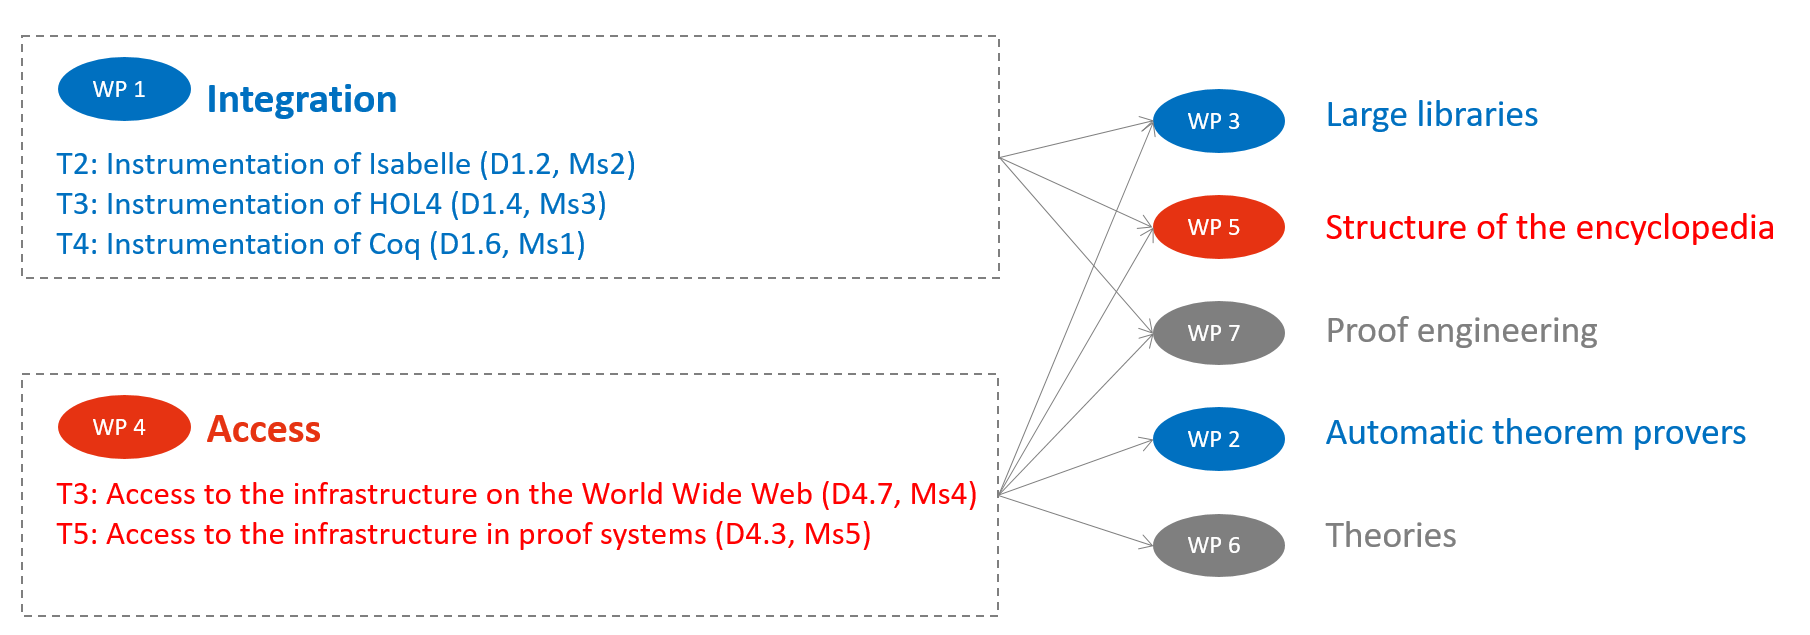
\includegraphics[width=\textwidth]{img/PERT}


%%% Local Variables:
%%%   mode: latex
%%%   mode: flyspell
%%%   ispell-local-dictionary: "english"
%%% End:


\subsection{Work Package List}\label{sec:wplist}

\begin{todo}{from the proposal template}
Please indicate one activity per work package:
RTD = Research and technological development; DEM = Demonstration; MGT = Management of the consortium
\end{todo}

%\makeatletter\wp@total@RM{management}\makeatother
\wpfigstyle{\footnotesize}
\wpfig[pages,type,start,end]

\newpage\subsubsection*{List of all deliverables}\label{sec:deliverables}

Here is an overview of the deliverables 
of the work packages. 

%In the table below, \emph{integrating work deliverables} (see top of
%section~\ref{sec:wplist}) are printed in boldface to mark them. They integrate
%contributions from multiple work packages.

{\footnotesize\inputdelivs{8cm}}

%%% Local Variables: 
%%% mode: latex
%%% TeX-master: "propB"
%%% End: 

\newpage\subsection{List of Milestones}\label{sec:milestones}

\begin{todo}{from the proposal template}
  Milestones are control points where decisions are needed with regard to the next stage
  of the project. For example, a milestone may occur when a major result has been
  achieved, if its successful attainment is a requirement for the next phase of
  work. Another example would be a point when the consortium must decide which of several
  technologies to adopt for further development.

  Means of verification: Show how you will confirm that the milestone has been
  attained. Refer to indicators if appropriate. For examples: a laboratory prototype
  completed and running flawlessly, software released and validated by a user group, field
  survey complete and data quality validated.
\end{todo}

\ednote{maybe automate the milestones}

\ednote{Rabe: I suggest having exactly 3 milestones, namely at months 18, 36, and 48 (corresponding to the EU's review schedule), possibly more milestones in the beginning e.g., at months 6 and 12}

\begin{milestones}
  \milestone[id=kickoff,verif=Inspection,month=1]
    {Organization setup}
    {Set up the organizational infrastructure of the project: mailing lists, web site, consortium agreement, activity tracking, \ldots}

  \milestone[id=logipedia-v1,verif=Inspection,month=12]
     {Logipedia v1}
     {Release of a first version of Logipedia with HOL Light standard library and parts of Matita standard library in 5 different systems: Coq, Matita, Lean, HOL and PVS}

  \milestone[id=coq-stdlib,verif=Inspection,month=24]
     {Coq in Logipedia}
     {Integration of most of Coq standard library in Logipedia}

  \milestone[id=isabelle-stdlib,verif=Inspection,month=24]
     {Isabelle/HOL in Logipedia}
     {Integration of most of Isabelle/HOL standard library in Logipedia}

  \milestone[id=compcert,verif=Inspection,month=36]
     {CompCert in Logipedia}
     {Integration of most of the CompCert library in Logipedia}

  \milestone[id=logipedia-v2,verif=Inspection,month=36]
     {Logipedia v2}
     {Release of a second version of Logipedia integrating important parts of the libraries of Isabelle, Coq, Matita and HOL4, and their translations in other systems}

  \milestone[id=atelierb,verif=Inspection,month=48]
     {Atelier B in Logipedia}
     {Release of a tool able to translate a complete development in Atelier B into a complete Dedukti proof}

\end{milestones}

%%% Local Variables: 
%%% mode: latex
%%% TeX-master: "propB"
%%% End: 

% LocalWords:  pn ednote verif ldots


\subsection{Work Package Descriptions}\label{sec:workpackages}
\begin{workplan}
  \newpage\begin{workpackage}[id=instrumentation,wphases=0-48,type=RTD,
  short=Instrument Provers,% for Figure 5.
  title=Instrument proof systems to produce Dedukti proof,
  lead=ISa,
  ISaRM=10]
  
\ednote{MK: We need one coordinating site. original coordinators: Frédéric Blanqui and
  Jesper Cockx}
\ednote{MK: interested parties (add their sites and RM here): David Deharbe,
Tobias Nipkow, Guillaume Genestier, Jesper Cockx, Guillaume Burel, Filip Marić, Makarius
Wenzel, Helmut Schwichtenberg, Nicolas Magaud, Gaspard Férey, Ulf Norell}

\begin{wpobjectives}
  The objective of this work package is to \ldots

This includes notably:
  \begin{compactitem}
  \item \ldots
  \end{compactitem}
  A key aspect will be to foster \ldots
\end{wpobjectives}


\begin{wpdescription}
We know how to express in Dedukti the theories implemented in Matita,
HOL Light, FoCaliZe, Coq, Agda, Lean, Minlog, Isabelle, HOL4,
Atelier B, and Rodin. The systems Matita, HOL Light, FoCaliZe, and
Coq, already have been instrumented to export proofs that can be
checked in Dedukti. Our first work package is to do the same thing for
Coq, Agda, Lean, Minlog, Isabelle, HOL4, Atelier B, and
Rodin. Three methods have to be used here: some of the systems
(Automath style), such as Coq, Agda, Lean, and Minlog already have
proof-terms that can be output, thus the main task is to translate
these proofs into the Dedukti format. Others (LCF style), such as
Isabelle and HOL4, have an inference kernel that can be
instrumented, and often already has, the main task here is to transform
the internal proof-object into an external proof-term. Others, such as
Atelier B and Rodin are slightly more difficult to address. For those,
we need to use the water ford method: extract an incomplete trace (a
sequence of lemmas) and fill the gap using automated theorem proving,
as experimented with Atelier B and Zenon.
\end{wpdescription}

\begin{tasklist}
\begin{task}[id=agda,title=instrument Agda]
[G\"oteborg, Delft]

Agda is a popular dependently typed programming language / proof
assistant based on Martin-L\"of’s intuitionistic type theory. Its theory
is similar to Coq and Lean, but is more focused on interactive
development and direct manipulation of proof terms (in contrast to
using a tactic language to generate the proof terms). Agda has a
sizable standard library (available at
https://github.com/agda/agda-stdlib) that consists of both utilities
for programming and mathematical proofs.


In the summer of 2019, Guillaume Genestier worked together with Jesper
Cockx on the implementation of an experimental translator from Agda to
Dedukti during a research visit at Chalmers University in Sweden. This
translator is still work in progress, but it is already able to
translate 142 modules of the Agda standard library to a form that can
be checked in Dedukti. This exploratory work uncovered several
challenges and opportunities for further work, which are outlined
below.

(1) To support the construction of proof terms, Agda provides powerful
features such as dependent pattern and copattern matching, eta
equality for functions and record types, and definitional proof
irrelevance. The first one – dependent pattern matching – can be
translated directly to rewrite rules in Dedukti. However, the two
latter features – eta equality and irrelevance – rely on Agda’s
type-directed conversion algorithm, while Dedukti’s conversion is
untyped. Hence in order to translate Agda proofs to Dedukti these
features need to be encoded.

One particular concern with the encoding of eta-equality is that in
general it requires storing of additional type information in the
proof terms. It can hence lead to a large blow-up in the size of those
proof terms, and thus greatly increase the cost of typechecking. The
same problem also occurs in other parts of Agda; for example
constructors of parametrized datatypes do not store the values of the
parameters, but they need to be reconstructed in the translation to
Dedukti. We plan to investigate two possible approaches to this
problem: either we can try to find a better encoding which reduces the
size of the type annotation, or alternatively we can extend the
Dedukti language with type-directed conversion rules to render the
type annotations unneccessary.

(2) Another unique feature of Agda is the support for first-class
universe level polymorphism. In particular, Agda has a built-in type
of levels that has complex structure of (in)equality between
levels. Compared to universe polymorphism in Coq, an additional
challenge is that levels in Agda can contain arbitrary terms as
subexpressions. Our plan is to define a sound and complete embedding
of Agda’s level type in Dedukti, based on the existing 1work on
encoding AC (associative-commutative) theories. This would both serve
as a stress test of how well Dedukti can handle complex equational
theories, and improve our understanding of type theories with
first-class universe level polymorphism, which would be useful for the
implementation of Agda.

(3) In contrast to Coq and Lean, Agda does not have a well-defined
core language to which proofs are elaborated. Instead, definitions are
translated to an internal representation that is relatively close to
the user input. This provides a challenge when translating Agda proofs
to Dedukti: each feature in Agda’s internal syntax needs to have its
own translation. As part of this project, we will hence investigate
possible designs for a core language for Agda. Having such a core
language would have several benefits: it would deepen our
understanding of the Agda language, it would increase the
trustworthiness of Agda proofs, and it would make it much easier to
export Agda terms to other languages (such as Dedukti in the context
of this project).

(4) Agda provides an experimental option for extending the language
with user-defined rewrite rules, which are very similar to the rewrite
rules provided by Dedukti. Because of this similarity, we expect it to
be straightforward to translate rewrite rules from Agda to
Dedukti. However, by comparing the two implementations we hope to gain
new insights and find opportunities for improvement on both sides. The
interest of some of these features goes beyond just the Agda
language. In particular, Lean also supports definitional proof
irrelevance, as does Coq with the recent addition of the SProp
universe. Hence we plan to collaborate with the teams working on those
languages to improve the support for these features where there is
overlap.

One research engineer at Chalmers, and one PhD student or postdoc at TU Delft.

Question: does this task belong to WP1 or WP2?


\end{task}

\begin{task}[id=lean,title=Instrument Lean]
[?]
\end{task}

\begin{task}[id=minlog,title=Instrument Minlog]
[LMU München]

The Minlog system <http://minlog-system.de> implements a theory of
computable functionals (TCF, cf. [SchwichtenbergWainer12], Ch.7).).
It is a form of higher order arithmetic where partial functionals are
first-class citizens.

The intended model of TCF is the Scott-Ershov model $C$ of partial
continuous functionals [Ershov77].  Computable functionals are defined
by so-called computation rules, a form of (possibly non-terminating)
defining equations understood as left-to-right conversion rules.  An
important example is the corecursion operator, which is needed to
define functions operating for instance on streams of signed digits (a
convenient format to represent real numbers).  The logical framework
allows to declare a proven equality as a rewrite rule.  Now it is
tempting to identify two terms or formulas when they have the same
normal form w.r.t. rewriting (including of course beta-conversion);
this is often called deduction modulo rewriting.  However, in a setup
like TCF where non-termination is allowed we cannot use normal forms,
but we can consider two terms or formulas as identical when they have
a common reduct.  This drastically simplifies proofs involving real
number arithmetic.

Another central feature of TCF (and hence the Minlog system) is that
it internalizes a proof-theoretic realizability interpretation (in the
form of Kreisel's so-called modified realizability, with realizers of
higher type).  More precisely, for every (co)inductive predicate we
have another one with one argument more, denoting a realizer.  It is
important that this realizers is expressed in the term language of TCF
(an extension of G\"odel's system $T$).  Since a realizer can be seen as
a program representing the computational content of a constructive
existence proof (expressing that a certain specification has a
solution), we now can reason about such programs in a formal way,
inside TCF.  In fact, given a proof M in TCF of a specification all x
ex y A(x,y) we can extract a term (program) t$_M$ and automatically
generate a new proof of all x A(t$_M$(x)).  In other words, for
programs generated in this way from existence proofs, formal
verification is automatic.  Note that for a proof involving
coinduction the extracted term contains the (non terminating)
corecursion operator.  Of course, for efficient evaluation in a second
step we want to translate our extracted term into an efficient
(functional) programming language like Haskell.

Other aspects of Minlog are more common.  It is a proof system in
Gentzen-style natural deduction and therefore based on proof terms
(the so-called Curry-Howard correspondence).  We distinguish between
(co)inductive predicates with and without computational content; in
fact, computational content only arises from (co)inductive predicates
marked as computationally relevant (c.r.).  In particular, both
universal und existential quantifiers do not influence computational
content: one needs to relativize them to c.r. predicates (like
totality) to make them computationally relevant.

A central application area of Minlog is to formalize Bishop-style
[Bishop67] constructive analysis and extract interesting algorithms
from proofs. An example is the Intermediate Value Theorem treated in
[LindstroemPalmgrenSegerbergStoltenberg08].  More recently we have
extracted algorithms operating on (both signed digit and Gray-coded)
stream-represented real numbers from proofs which never mention
streams.  They come in by relativizing real number quantifiers to
appropriate coinductive predicates [Berger09].

The work planned to be done by the Minlog group is to extend this kind
of work further into constructive analysis, e.g. Euler's existence
proof of solutions of ODEs.  We would like to learn from the
experience of other proof assistant developers working on related
matters, both conceptually and by sharing libraries.  It would be very
helpful if this can be done in a unified setting where different
approaches can be compared.

Here we need to go a little futher and propose to express Minlog
proofs in Dedukti.

One Postdoc and one Phd position

\end{task}

\begin{task}[id=isabelle,title=Instrument Isaabelle]
[TU München]

Isabelle as a logical framework \cite{paulson700} is an intermediate
between Type-Theory provers (like Coq or Agda) and classic LCF-style
systems (like HOL Light or HOL4). The inference kernel can already
output proofs as $\lambda$-terms on request, but this has so far been
only used for small examples \cite{Berghofer-Nipkow:2000:TPHOL}. The
challenge is to make Isabelle proof terms work routinely for
reasonably big entries from The Archive of Formal Proofs
\cite{isabelle-afp}. Preliminary work by Wenzel (2019) has
demonstrated the feasibility for relatively small parts of
Isabelle/HOL: some orders of magnitude in scalability are still
missing.

This work package will revisit important aspects of the Isabelle/HOL
logic implementation on top of the Isabelle/Pure framework, such as
normalization of proofs, efficient type-class reasoning, special
representation of derived rules and definition principles (datatypes,
recursion, induction). The volume of proof term output may be reduced
further, by taking more structure of the target language (Dedukti)
into account and omitting certain low-level reasoning of HOL (e.g.\
for inductive types). [Subcontracted to Makarius Wenzel, Augsburg,
Germany.]

The underlying Isabelle/ML implementation platform (on top of Poly/ML)
will be revisited as well, to improve monitoring of memory usage, and
to double the standard heap size from 16\,GB to 32\,GB (without
suffering from the full overhead of the 64\,bit
addressing). [Subcontracted to David Matthews, Edinburgh, UK.]

\end{task}

\begin{task}[id=HOL4,title=Instrument HOL4]
[G\"oteborg]

The HOL4 proof assistant is home to a few medium to large scale
specifications and associated proof developments that have value
outside of HOL4. These specifications include the formal semantics of
the CakeML language (and its verified compiler) and an extensive
specification of the ARM instruction set architecture (ISA) as
formalised by Anthony Fox at the University of Cambridge.

HOL4 has support for exporting proofs to the OpenTheory proof exchange
format, and there has been some work on importing OpenTheory proofs
into Dedukti. However, the current state of these techniques and their
implementations does not scale to real examples such as those
mentioned above.

This part of the project will be about re-thinking and re-designing
the tools HOL4-to-OpenTheory and OpenTheory-to-Dedukti tools such that
they scale to the point where real examples of interest, such as those
mentioned above, can be exported.

2 Person Years at Chalmers


 \end{task}

\begin{task}[id=atelier-b,title=Instrument Atelier-B]
\ednote{Southhampton, Toulouse, Clearsy writes this}
\end{task}
\begin{task}[id=rodin,title=Instrument Rodin]
\ednote{Southhampton, Toulouse, Clearsy}
\end{task}
\begin{task}[id=matita,title=integrate the translator to Matita in Matita itself and export the full Matita library]
\ednote{Bologna}
\end{task}
\end{tasklist}

\begin{wpdelivs}
  \begin{wpdeliv}[due=3,miles=startup,id=requirements,dissem=PU,nature=DEM,lead=ISa]
      {Requirements Analysis and Synchronization}
\end{wpdeliv}
\end{wpdelivs}
\end{workpackage}

%%% Local Variables:
%%% mode: latex
%%% TeX-master: "../propB"
%%% End:

  \newpage\begin{workpackage}[id=theories,type=RTD,wphases=1-48,
  short=Theories,% for Figure 5.
  title= Theories,
  activity=jra,
  lead=Inn,
  BiaRM=70,
  BirRM=3,
  IasRM=5,
  InnRM=12,
  InrRM=83,
  LeeRM=3,
  LmuRM=16,
  MedRM=4,
  ProRM=11,
  RunRM=7,
  wphases=1-48,
  ]

\begin{wpobjectives}
  This work package addresses proof systems that are currently at LIL 0, i.e.\
  whose logic and theories have not yet been expressed in Dedukti. Our
  objective is to bring them to LIL 2 or better over the duration of the
  project so that at least elementary proofs can be exported and checked in
  Dedukti.

  Achieving these goals requires (i) expressing the logics
  that underlie these systems in Dedukti and
  (ii) instrumenting the original proof systems so that they can export proofs
  that can be checked in Dedukti. Much of the work required in this work package
  is of foundational nature.
\end{wpobjectives}
\begin{wpdescription}
  The tasks are presented according to the individual systems. Nevertheless,
  the project addresses cross-cutting concerns and foundational aspects such
  as set-theoretic vs.\ type-theoretic foundations, predicate and dependent
  types, (co-)recursive definitions and (co-)inductive proofs and so on. The
  network established in this project will avoid ``reinventing the wheel'', also
  taking advantage of the experiences of the more mature systems considered in
  \WPref{instrumentation} and of the work carried out in \WPref{atpetc}.
\end{wpdescription}

\begin{tasklist}
% \begin{task}[id=abella,title=Express the theory of Abella in Dedukti,shorttitle=Abella]
%   \ednote{K. Chaudhuri, Saclay}
%   \begin{enumerate}
\item Encoding proofs on finite structures: model checking queries supported by
  Abella's Bedwyr prover rely on the exhaustive exploration of finite structures
  and support quantifier alternation. Representing such proofs in Dedukti
  involves alternating phases of deduction and computation. A particular
  challenge is handling backtracking search, which is different from Dedukti's
  notion of computation as confluent rewriting.
\item Encoding cyclic proofs: Abella's implementation of (co-)induction is based
  on cyclic reasoning with size annotated relations. A representation in Dedukti
  requires extracting explicit invariants from cyclic proofs.
\item Equality and unification: Abella's equality proofs examine complete sets
  of unifiers for terms assumed to be equal, based on a trusted unification
  engine. The unification procedure can be recast as a rewrite system in
  Dedukti, but it remains to derive facts from the unifiability of terms.
\item Support $\lambda$-tree syntax: an encoding of Abella in Dedukti requires
  $\lambda$-terms to be considered modulo $\alpha\beta\eta$-equivalence, which
  is not natively supported. Moreover, for reasoning about the inductive
  structure of terms, Abella provides the $\nabla$-quantifier, which provides a
  challenge for representing the full logic in Dedukti.  
\end{enumerate}

%%%%% OLD TEXT %%%%%
% The usual approach to capturing either Peano and Heyting arithmetics
% is to use various axioms (and an axiom scheme for induction) on top of
% classical and intuitionistic first-order logic.  Indeed, this is the
% approach used in the Dedukti proof checker.


% A different approach to encoding arithmetic has been developed over
% the past 20--30 years, starting with papers by Schroeder-Heister and
% Girard in the early 1990s and extended in a series of papers by
% Baelde, Gacek, McDowell, M, Momigliano, Nadathur, and Tiu.  In this
% new setting, first-order logic is extended by considering both
% equality and the least fixed point operator as \emph{logical
%   connectives}: these logical connectives are not available directly
% in Dedukti.

% This new foundations for arithmetic has been implemented in two
% systems: the automated Bedwyr prover and the interactive Abella
% prover.  While neither Bedwyr nor Abella are as popular as many of the
% theorem provers that are covered by this proposal, there are two
% important reasons to consider incorporating them into the Logipedia
% effort.

% First, the Bedwyr prover is capable of constructing proofs for the
% kind of queries that are part of \emph{model checkers}.  This class of
% provers has not yet been incorporated into Dedukti.  The
% proof-theoretic work behind model checking in Bedwyr should provide
% some of the insights needed for allowing Dedukti to proof check the
% results of model checkers.

% Second, Bedwyr and Abella provide for direct and elegant support of
% meta-level reasoning.  Given that the foundations for Bedwyr and
% Abella have been given using Gentzen's sequent calculus, it was
% possible to enrich their foundations to allow for the treatment of
% binding structures within terms.  As a result, it is possible to
% reason directly on terms representing $\lambda$-terms and
% $\pi$-calculus expressions.  In particular, the Abella prover has
% probably the most natural and compact formal treatment of the
% $\pi$-calculus and its meta-theory when compared to all other attempts
% in any other theorem provers.  More generally, the Abella prover
% should be able to treat the meta-theory of programming and
% specification languages as well as various logics and their
% proofs. While these tasks are not the typical tasks considered by the
% majority of theorem provers within the scope of this proposal,
% meta-theory results do play an important role at times: in fact, the
% ultimate questions as to whether or not a proof checkers (such as that
% used by Dedukti) is correct or not will involve meta-theoretic
% questions.

% We propose to work on the general problem of exporting proofs from
% Abella to Dedukti.  (Since all proofs that are constructed
% automatically via Bedwyr can also be constructed manually within
% Abella, we shall limit our discussion below to Abella only.)  The
% proposed work will serve not only to answer the question of how to
% relate these two different foundations for arithmetic but also to
% allow Abella's particular style of proofs to find applications in the
% wider world of formalized proofs.

% The general problem described above has the following constituent parts.

% (1) Proofs involving searching finite structures. Proofs built for
% model checking problems over finite structures have two different
% kinds of phases.  To illustrate, consider trying to find a specific
% node within a binary tree.  If such a node exists, then the proof
% essentially encodes the path to the node in the tree.  If, however, no
% such node exists, then the proof of that negative fact is essentially
% a computation that exhaustively explores the tree.  Using the Dedukti
% terminology: in the first case, the proof involves several deduction
% steps, while in the second case, the proof involves a pure
% computation. When dealing with model checking problems such as
% simulation (in concurrency theory) and winning strategies (in game
% theory), proofs will involve alternating phases involving either
% deduction or computation.  Since the notion of computation in
% Abella-style proofs involves backtracking search, that style
% computation will be quite different from Dedukti's notion of
% computation as confluent rewriting.

% (2) Extending model checking problems to the general case of infinite
% structures and the associated inductive reasoning methods. Although
% the formal basis of Abella uses least and greatest fixed-point
% combinators and explicit (co-)invariants, the Abella implementation of
% (co-)induction is based on cyclic reasoning using size-annotated
% relations. It is known, in principle, how to convert cyclic proofs
% using annotations to proofs with explicit invariants, but an invariant
% extraction procedure that works in all cases is still missing. Once
% such invariants are available, incorporating them into Dedukti should
% be straightforward in association with part (1).

% (3) Binding structures. Abella, as well as several other computational
% logic systems ($\lambda$Prolog, Isabelle/Pure, Twelf, Beluga, etc)
% make use of the so-called \emph{$\lambda$-tree syntax} (a form of
% \emph{higher-order abstract syntax}, HOAS) approach to represent
% bindings. This approach is further enriched in Abella with the
% $\nabla$-quantifier that allows inductive and co-inductive properties
% to be defined based on the \emph{structure} of $\lambda$-terms. We
% propose to examine encodings of $\lambda$-tree syntax in Dedukti. The
% best approach probably involves extending the underlying theory of
% Dedukti with a quantifier similar to Abella's $\nabla$-quantifier.

% (4) Reflective treatment of unification. One of the features of
% Abella's style of proofs is the use of left-introduction rules for
% equality that exhaustively examine complete sets of unifiers for
% $\lambda$-terms. This is implemented in terms of a unification engine
% that is currently a trusted black box, which complicates any proposal
% for exporting proofs to different implementations of unification or
% equality. In Dedukti the unification procedure can be recast as a
% rewrite system, but it is unclear how to derive reflective properties
% based on the unifiability of terms.

% \end{task}

\begin{task}[id=hott,
  title=Express Cubical Type Theory in Dedukti,
  shorttitle=CuTT,
  lead=Inr, % B. Barras
  InrRM=42, % 36 PhD + 6 in kind B. Barras
  BirRM=3,  % 3 in kind B. Ahrens
  LeeRM=3,  % 3 in kind N. Gambino
  wphases=1-48,
  ]
  \vspace{-5mm}
  \begin{compactitem}
  \item Express 2-Level Type Theory (2LTT) as an object theory in Dedukti, as
    a stepping stone towards encoding more expressive variants of homotopy type
    theory.
  \item Express a core Cubical Type Theory (CubTT) in 2LTT: here, the main challenge is
    that equality in cubical type theory is more expressive than what can be
    expressed through rewrite rules in Dedukti.
  \item Define structures such as cartesian cubical type theory on top of the
    core, and compare these structures.
  \item Import the UniMath library into Dedukti and translate it into Cubical
    Type Theory. The UniMath library extends a version of
    Martin-Löf type theory by the univalence axiom. It provides an interesting
    case study for our encoding of CubTT.
  \end{compactitem}
\end{task}

\begin{task}[id=matching,
  title=Express Matching Logic in Dedukti and instrument the K prover,
  shorttitle=K,
  lead=Ias,
  IasRM=5,
  RunRM=7,
  wphases=1-36,
  ]
  \vspace{-5mm}
  \begin{compactitem}
  \item Express Kore in Dedukti: Kore is the specification language used for
    describing Matching Logic theories in K and will serve as the interface
    between the K prover and Logipedia.
  \item Instrument the K prover to produce detailed proof traces expressed in
    Kore.
  \item Integrate an instrumented automated prover (cf.\ tasks
    \taskref{atpetc}{instrumenting} and \taskref{atpetc}{tracetodedukti}) into
    the K prover for obtaining proofs for the queries generated by the K prover.
  \item Combine the translations into Dedukti from Kore and from the automated
    prover into a single Dedukti proof.
  \end{compactitem}
\end{task}

\begin{task}[id=minlog,
  title=Express the theory of Minlog in Dedukti,
  shorttitle=Minlog,
  lead=Lmu,
  LmuRM=16, % 10 post-doc + 6 in kind H. Schwichtenberg + K. Miyamoto
  wphases=1-30,
  ]
  \vspace{-5mm}
  \begin{compactitem}
  \item Further develop and implement extensional realizability in Minlog as
    a necessary first step for bridging Minlog and Dedukti.
  \item Express the core Minlog logic and proofs in Dedukti, benefitting from
    the work on realizability for exporting programme extraction to Dedukti.
  \item Properly encode coinduction and corecursion in Dedukti: these concepts are
    fundamental to Minlog, for example for representing real numbers as streams of
    digits, but they are not native to Dedukti.
  \item Import a subset of Dedukti into Minlog, apply program development by proof
    transformation, and export back. This will make Dedukti a usable tool for the
    development of proofs and programs in constructive analysis and allow Minlog
    users to benefit from theories formalized using other proof assistants.
  \end{compactitem}
\end{task}

\begin{task}[id=mizar,
  title=Express the theory of Mizar in Dedukti,
  shorttitle=Mizar,
  lead=Bia,   % Artur Korni{\l}owicz
  BiaRM=70, % 48 post-doc + 22 in kind
  InnRM=12,   % 9 post-doc + 3 C. Kaliszyk
  wphases=1-48,
  ]
  \vspace{-5mm}
  \begin{compactitem}
  \item Express the foundations of Mizar (first-order Tarski-Grothendieck set
    theory) in Dedukti, together with Mizar's soft
    type system. Take advantage of Dedukti's rewriting capabilities to automate
    parts of type inference.
  \item Instrument Mizar to export type disambiguation data. Exporting the
    information present in the Mizar types will enable us to optimize the
    representation of Mizar statements in Dedukti.
  \item Express Mizar's equality checking and unification steps as a mix of
    small proof steps and rewrite rules so that Dedukti's proof kernel can
    verify them. Export necessary semantic information that is not currently
    available outside of the Mizar checker in order to check the basis of the
    Mizar library and make it available in Logipedia.
  \end{compactitem}
\end{task}

\begin{task}[id=pvs,
  title=Express the theory of PVS in Dedukti,
  shorttitle=PVS,
  lead=Inr,   % Gabriel Hondet
  InrRM=20,  % 20 in kind G. Hondet
  wphases=1-48,
  ]
  \vspace{-5mm}
  \begin{compactitem}
  \item Extend the existing encoding in Dedukti,
    restricted to a fragment of PVS with decidable type checking, and represent
    proofs of type checking conditions for predicate subtypes.
  \item Instrument PVS to export proof traces to Dedukti given that PVS proof
    tactics do not produce proof terms.
  \item Design and implement a PVS proof checker in Dedukti based on the
    reconstruction of proof traces exported from PVS.
  \end{compactitem}
\end{task}

\begin{task}[id=smart,
  title=Express Smart models and proofs in Dedukti,
  shorttitle=Smart,
  lead=Pro,   % Stephane Lescuyer
  ProRM=11,
  wphases=1-48,
  ]
  \vspace{-5mm}
  \begin{compactitem}
  \item Choose a viable translation strategy from Smil programs (the
    intermediate form of Smart models used by ProvenTools) into Dedukti
    by experimenting with direct translations or translations through a
    different tool such as Coq or Why3.
  \item Develop a prototype capable of translating the definitions and proof
    obligations corresponding to relevant examples from the Smart
    standard library.
  \item Integrate the prototype into ProvenTools: integrate proof rules internal
    to the prover and evaluate the scalability to cross-verifying real-world use
    cases.
  \end{compactitem}
\end{task}

\begin{task}[id=tla,
  title=Express the theory of \tlaplus in Dedukti,
  shorttitle=\tlaplus,
  lead=Inr,   % Stephan Merz
  InrRM=21,   % 18 post-doc + 3 in-kind S. Merz
  MedRM=4,
  wphases=1-48,
  ]
  \vspace{-5mm}
  \begin{compactitem}
  \item Express the untyped \tlaplus set theory with choice in
    Dedukti.
  \item Instrument backends of the \tlaplus Proof System to export proofs,
    taking advantage of Dedukti's rewriting capabilities in order to compress
    the size of proofs.
  \item Formalize a distributed assignment of rehabilitation programs to
    patients and updates of the process in MED-EL's software.
  \end{compactitem}
\end{task}

\end{tasklist}

\begin{wpdelivs}
  \begin{wpdeliv}[due=18,id=wp2midterm,dissem=PU,nature=R,lead=Inn]{Report on defining theories in Dedukti}\end{wpdeliv}

  \begin{wpdeliv}[due=48,id=wp2cubical,dissem=PU,nature=R,lead=Inr,task=hott]{Report on the integration of Cubical Type Theory in Dedukti}\end{wpdeliv}

  \begin{wpdeliv}[due=36,id=wp2matching,dissem=PU,nature=R,lead=Ias,task=matching]{\hspace{-2mm}Report on the integration of Matching Logic}\end{wpdeliv}

  \begin{wpdeliv}[due=48,id=wp2minlog,dissem=PU,nature=R,lead=Lmu,task=minlog]{Report on the integration of Minlog}\end{wpdeliv}

  \begin{wpdeliv}[due=48,id=wp2mizar,dissem=PU,nature=R,lead=Bia,task=mizar]{Report on the integration of Mizar}\end{wpdeliv}

  \begin{wpdeliv}[due=48,id=wp2pvs,dissem=PU,nature=R,lead=Inr,task=pvs]{Report on the integration of PVS}\end{wpdeliv}
  
  \begin{wpdeliv}[due=48,id=wp2smart,dissem=PU,nature=R,lead=Pro,task=smart]{Report on the integration of Smart}\end{wpdeliv}
  
  \begin{wpdeliv}[due=48,id=wp2tlaplus,dissem=PU,nature=R,lead=Inr,task=tla]{Report on the integration of \tlaplus}\end{wpdeliv}
\end{wpdelivs}
\end{workpackage}


%%% Local Variables:
%%% mode: latex
%%% TeX-master: "../propB"
%%% End:

  \newpage\begin{workpackage}[id=libraries,wphases=0-48,type=RTD,
  short=Libraries,% for Figure 5.
  title=Libraries,
  lead=Inr,
  InrRM=10,
  TumRM=39]
%TUM: 24 for Analysis library, 12 for CakeML,
%TUM: 3 for AFP/Makarius (25k EUR) - the latter do not generate overheads!


\ednote{MK: We need one coordinating site. original coordinators: Georges Gonthier and
Tobias Nipkow} \ednote{MK: interested parties (add their sites and RM here): David
Deharbe, Nicola Gambino, Tobias Nipkow, Makarius Wenzel, Julien Narboux, Gaspard Férey,
François Thiré, Magnus Myreen}

\begin{wpobjectives}
The objective of this WP is to export large dedicated libraries in curated form to Dedukti
for access to end-users. The focus is \emph{Access} and \emph{Scalability}.
\begin{compactitem}
\item This WP is responsible for supplying the lion's share of proofs for
the Dedukti data base.  As a result it will be a stress test for the
results of \WPref{instrumentation}: is the proof infrastructure
capable of processing truly large amounts of material/proofs?

\item The target libraries are dedicated to particular application
areas. They provide a substantial coverage of that application area
and do so in a structured manner. This may require reworking the
libraries for better access.

\item The libraries are curated for end-user application. That is, they
are structured according to application specific ontologies that
support browsing and search. The structuring leverages the
infrastructures of \WPref{structuring} and will be a
stress test for the results of \WPref{structuring}: is the metadata
infrastructure capable of representing the structure of large
libraries?
\end{compactitem}
\end{wpobjectives}


\begin{wpdescription}
Translating the standard libraries of the systems is part of the \WPref{instrumentation}.
This WP focusses on advanced libraries selected according to the following criteria:
\begin{compactitem}
\item Relevance: the libraries should support core areas of matematics and computer science.
\item Coverage: the libraries should have a wide coverage of an application area.
\item Maturity: the libraries should have been used in a significant application already.
\end{compactitem}
As a result we selected the following libraries: MathComp, Coq's revised
Analysis library, the Archive of Formal Proofs, Isabelle's revised Analysis and Probability library,
GeoCoq, Flyspeck and CakeML. In the future we plan to incorporate
CompCert, seL4, and selected Mizar and PVS libraries (once Mizar and
PVS have reached LIL 2).
\end{wpdescription}


\begin{tasklist}
\begin{task}[id=mathcomp,title=MathComp]
\ednote{Sophia, Saclay (Gonthier), Paris}
\end{task}

\begin{task}[id=milc,title=Revised Coq Analysis Library]
\ednote{Saclay (Boldo), Paris, Sophia}
\end{task}

%\begin{task}[id=mizar,title=The Mizar library]
%\ednote{Innsbruck, Bialystok}
%\end{task}

\begin{task}[id=afp,title=Isabelle's Archive of Formal Proofs]
\ednote{TU München (Wenzel)}

Isabelle's Archive of Formal Proofs (AFP) \cite{isabelle-afp} is a
growing user-contributed online library for Isabelle. In Feb-2020, the
AFP consisted of more than 500 entries (articles of formalized
mathematics) by 340 authors, and required approx. 60h CPU time for
checking (using many gigabytes of memory).  The purpose of this task
is to scale up the Isabelle instrumentation for Dedukti further, to
cover major parts of this library. We do not intend to restructure or
document the library further beyond what is provided by the authors of
each article and by the hierarchical dependencies among the articles.

The key challenge is scaling. The ultimate aim is to export the main
substance of the AFP without promising full coverage: some entries
with prohibitive resource requirements will be omitted. Also note that
the AFP is continuously growing at a high rate and thus a moving
target.
\end{task}

\begin{task}[id=isaAnalysisProb,title=The Isabelle Analysis \& Probability library]
\ednote{TU München (Nipkow)}

The Isabelle Analysis and Probability Theory library consists of more than
200.000 lines of definitions and proofs, corresponding to almost 4000 printed
pages. It covers topology, homology, multivariate, functional and complex
analysis, measure and probability theory, and a dedicated library for
ordinary differential equations. It is fair to say that it is the most
advanced machine-checked library in the area of analysis and probability
theory.\footnote{The Isabelle analysis and probability theory library is
in part based on the extensive library of the HOL Light system but has
generalized it from real numbers to appropriate algebraic structures and
includes areas absent from the HOL Light library (in particular measure
theory and ordinary differential equations).} It is currently used by 60 out
of 500 articles in the Archive of Formal Proofs, a user-contributed library
of Isabelle/HOL proofs from all areas of computer science and
mathematics. Moreover, it is the only existing library in this area where
proofs are structured and readable. Due to its size and generality and
because analysis and probability theory are pervasive in any application in
the engineering and natural sciences and economics, this library will be a
KER of the project: it is a fundamental enabling resource for almost any
formal verification activity in these areas, for example autonomous driving
and mathematical finance. The purpose of this task is to structure, document
and develop this library for optimal accessibility, ease of use and
comprehensiveness. The aim is a curated library for applications.

Any library is only as useful as its structure and documentation, no matter
how sophisticated the search facilities are. Therefore the primary aim of
this task is to make this library easily accessible. At the same time the
library needs to be developed further: some material needs revising for ease
of use and some essential material needs to be added.

\textbf{Accessibility}\quad
The library is a large collection of theories with a hierarchical dependency
relation. However, this structure has grown over time and does not always
reflect the abstract mathematical dependencies. In short, the structure needs
to be modularized. This requires a significant refactoring effort.
%
At the same time we need to add metadata to the source material to turn this
structured collection of theorems and proofs into a curated library at the
Dedukti level.  This is where we need to interface with \WPref{structuring}. We
will be test drivers of the metadata infrastructure provided by that WP, in
particular the ability to describe ontologies for structuring in the large.
This will also entail annotating those statements in the library that
correspond to proper mathematical theorems as opposed to auxiliary lemmas
required only for the benefit of the theorem prover.
To increase accessibility we will also include links from the library into
Wikipedia and in particular in the other direction to raise the awareness
of Dedukti.

\textbf{Development}\quad
Although the library support for integrals is extensive, it suffers
from the (necessary) coexistence of different kinds of
integrals. This complicates proofs about integrals in applications and needs
to be unified, which entails further refactoring. The rest of the
development adds further essential material:
1. Fourier analysis because of its extreme important both for pure mathematics and for
engineering and physics (especially the Fourier
transform). A formalization of basic properties of the Laplace transform is already available in the AFP. 2. Stability theory for differential equations and
dynamical systems, in particular Lyapunov functions, because of their
relevance for the verification of cyber-physical systems.
3. Stochastic differential equations to model a large range of
dynamical systems with stochastic components, from physics to financial markets.
\end{task}

\begin{task}[id=geocoq,title=The GeoCoq library]
\ednote{Sophia (Boutry), Strasbourg, Belgrade}
\end{task}

\begin{task}[id=flyspeck,title=The Flyspeck library]
\ednote{Saclay (Grienenberger)}
The
\textsc{HOL Light} library is especially large and varied.
    
First, its standard library contains definitions of the logical connectives,
pairs, natural and real numbers, well-founded relations, lists, sets, and usual
results concerning these objects. The standard library also contains tools to
define inductive types, iterate operations, execute calculations over natural
and real numbers, integers, and rationals. Many more libraries are added to
this basis, formalizing many mathematical fields, objects, and results, for
example arithmetics, complex numbers, group and ring theory, orderings, first
order logic, Hilbert axiomatic geometry, complex function vector spaces,
geometric algebra, quaternions, IEEE floating-point numbers, Jordan curves.

One of those libraries, particularly large and unique, is the multivariate
analysis library
\footnote{\url{https://github.com/jrh13/hol-light/tree/master/Multivariate}},
which spans the fields of metric spaces, topology, homology, linear algebra,
convexity, real and complex analysis and transcendentals, derivatives, and
integration. This profusion of multivariate analysis theorems was partly
motivated by the \textsc{Flyspeck} project.

The \textsc{Flyspeck} project gives a formal proof of the \textsc{Kepler}
conjecture. The statement and proof is based on an original proof of Thomas
\textsc{Hales} \cite{DBLP:journals/corr/HalesABDHHKMMNNNOPRSTTTUVZ15},
and entirely formalized and proved in \textsc{HOL Light}
\footnote{\url{https://github.com/flyspeck/flyspeck}}.
    
This variety and multitude of formalized mathematical results, sometimes unique
to this system, motivates the project of importing the \textsc{HOL Light}
library and \textsc{Flyspeck} project in the \textsc{Dedukti} system, in view
of its integration into \textsc{Logipedia}.
 
Proofs coming from the HOL systems, including \textsc{HOL Light}, are known to
be very large, adding to the already existing issue of the scalability of
exporting software for large libraries
\cite{DBLP:conf/tphol/Wong95,DBLP:conf/cade/ObuaS06,DBLP:conf/itp/KellerW10,
DBLP:conf/cade/Kumar13}. As an example, the size of the standard library is
1.5M in \textsc{HOL Light} files (i.e. .ml files), while the same files once
exported as \textsc{Dedukti} files scale to 2G, and the whole
\textsc{HOL Light} library and the \textsc{Flyspeck} project are each as
large as 30M. The multitude of automatic tactics and their increasing
complexity and number of dependencies suggests that the generation time, size,
and rechecking time of exported proofs will not increase linearly. Scalable
export techniques \textsc{HOL Light} proofs have been investigated
\cite{DBLP:conf/itp/KaliszykK13} and can provide a solid base to
this project; for want of significantly reducing the size of generated
\textsc{Dedukti} files, the time of export could at least be reduced.

The main milestones of this task are the further automation of the translation
from \textsc{HOL Light} to \textsc{Dedukti}, the import of the multivariate
analysis library, the import of the whole \textsc{HOL Light} library, and the
import of the \textsc{Flyspeck} in \textsc{Dedukti}.
\end{task}

\begin{task}[id=cakeml,title=The CakeML compiler library]
\ednote{Chalmers (Myreen), Strasbourg, TU München}
The CakeML compiler library consists of the CakeML programming language
definition, its compiler and the correctness proofs about the
compiler. This is a cutting edge compiler library and one of only two
verified compilers for real languages, the other being CompCert. Its
export to Dedukti is one of the KERs of this project. Because of the
size and importance of this library, we will approach the export from
two angles.

The first approach utilizes OpenTheory-based technology. The CakeML
compiler development lives within the HOL4 prover. HOL4 can export
definitions and proofs in the OpenTheory format, which can in turn be
translated into Dedukti. This link from HOL4 via OpenTheory to Dedukti
exists but, in its current state, fails to scale to the task of
transporting something as sizeable as the CakeML compiler
development. This part of this task will rework the route via
OpenTheory to scale better, possibly taking inspiration from an
OpenTheory-like approach that scaled well for the HOL light
prover~\cite{KaliszykK13}.

The second approach establishes a connection from HOL4 via Isabelle to
Dedukti. The basis is a promising new approach of virtualizing HOL4
inside Isabelle \cite{ImmlerRW19}. That is, the inference
kernel of HOL4 is replaced by that of Isabelle and the resulting
system produces Isabelle theorems instead of HOL4 theorems. This has
the invaluable additional benefit that tools, not just theorems, can
be shared. As a benchmark of the viability of this approach we plan to
export CakeML via Isabelle to Dedukti.
\end{task}

By Arthur Chargueraud
{\bf Trusted chain}

A grant challenge in program verification is that of running trusworthy
software on trustworthy hardware. This challenge can be decomposed in
four steps: (1) formally verify the source code of the program,
(2) compile this code using a formally-verified compiler,
(3) launch the program on a formally-verified operating system,
(4) running the whole thing on hardware with formally-verified circuits.

Developing a program verification framework, a verified compiler, a
verified operating system, and a verified hardware, corresponds to 4
daunting tasks. Just setting up a reasonable proof-of-concept takes of
the order of 10 man-year of work. Raising the bar to a production-ready
tool takes at least Can additional order of magnitude in terms of efforts.

Considerable progress has been made on these three aspects
over the past decade, and every year the technology becomes more mature.
Yet, there is a pitfall. The tools are not all developed using the same
theorem prover, not just for historical reasons but also because different
proof assistants have appeared better-suited at different tasks.

In that setting, how one could possibly complete a trustworthy chain if
the four main pieces of the chain are not properly hooked to one another?
As a concrete example, CFML is a program verification for verifying ML code,
developed in Coq; and CakeML is a verified compiler for ML code,
developed in HOL4. How can we combine the two tools to produce verified
machine code from verified ML code?

There are two main ways to address the issue. One way is to port the
proofs of all the formalized tools into a same proof assistant.
Doing so might be possible in a far future, however given the scale and
the complexity of the tools, this approach does not provide a short-term
solution. Another, more accessible approach consists of translating
between proof assistants only the formal statements associated with the
interfaces between the 4 pieces of the verified chain.

Concretely, the interfaces involve: (1-to-2) a formal semantics for
a programming language, (2-to-3) a formal semantics for a set of
system calls (the OS API and isolation model), (2-and-3-to-4) a formal
semantics for machine code (instruction set and memory model).
Translating such formal interfaces, which consists solely of statements,
is considerably easier than translating all the verification proofs
associated with the tools.

A proposal for translating such interfaces should satisfy the following
requirements. First, the translations must to be trusworthy. In particular,
translation by hand is not an option, and developing translation tools
between every pair of provers might make the trusted code base prohibitively
large. Second, the translations should be maintainable. Indeed,
formal specifications of the aforementioned interfaces do evolve, slowly but
surely, through time, in particular for incorporating new features.
Third, the translations should produce formal definitions that are written
in a style sufficiently idiomatic with respect to the target proof assistant.
Indeed, carrying out proofs with respect to definitions in non-idiomatic
style induce prohibitive overheads.

We propose to tackle the problem by leveraging the unifying language
Dedukti in the following way. Assume that we have, for formal statements,
a bi-directional translations between each prover and Deduki. Then,
we could translate a formal interface from one system to another.
The user may then provide alternative, more idiomatic statements for
specific definitions, and prove (by hand) that the alternative definitions
are equivalent to the automatically-generated ones. If the original
interface is modified, then the automatic translations can be updated,
and the proof system would notify the user of which alternative definitions
need to be updated accordingly.

For example, we could take CakeML's semantics of its input ML language,
translate it automatically into Dedukti, then translate Dedukti's
definition into Coq, refine by hand a few definitions to make them more
idiomatic, and obtain a usable Coq semantics, with respect to which
the correctness of the CFML verification tool can be established in Coq.
Completing this case study is motivating not only because it delivers
an immediate result of relating two existing tools, but also because it
would validate the general approach of translating semantics via Dedukti
in a realistic manner.

Beyond this one example, other motivating case studies will be considered,
such as translating the formal semantics of ComCert-C into other proof
assistants, or translating the formal semantics of ARM instruction set.

%\begin{task}[id=unimath,title=The UniMath library]
%\ednote{Birmingham (Ahrens)}
%\end{task}

%\begin{task}[id=pvs,title=The NASA PVS library]
%\end{task}
%\begin{task}[id=sel4,title=The seL4 library]
%\end{task}

%\begin{task}[id=compcert,title=The CompCert library]
%\end{task}
\end{tasklist}

\begin{wpdelivs}
  \begin{wpdeliv}[due=3,miles=startup,id=requirements,dissem=PU,nature=DEM,lead=Inr]
      {Requirements Analysis and Synchronization}
\end{wpdeliv}
  \begin{wpdeliv}[due=36,miles=isabelle-stdlib,id=requirements,dissem=PU,nature=DEM,lead=Tum]
      {Scalable export of proof terms for major parts of Isabelle/AFP}
  \end{wpdeliv}
\end{wpdelivs}
\end{workpackage}

%%% Local Variables:
%%% mode: latex
%%% TeX-master: "../propB"
%%% End:

  \newpage\begin{workpackage}[id=atpetc,wphases=0-48,type=RTD,
  short=ATPs etc.,% for Figure 5.
  title={ATP, SAT, SMT, Model checkers},
  lead=Lie,
  LieRM=10]

\ednote{MK: interested parties (add their sites and RM here): Guillaume Burel, Raphaël Cauderlier, David Deharbe, Pascal Fontaine, Emilio J. Gallego Arias, Olivier Hermant, Cezary Kaliszyk, Chantal Keller, Filip Marić, Stephan Merz, Dale Miller, Julien Narboux, Martin Suda, Josef Urban}

\begin{wpobjectives}
  The objective of this work package is to \ldots

This includes notably:
  \begin{compactitem}
  \item \ldots
  \end{compactitem}
  A key aspect will be to foster \ldots
\end{wpobjectives}


\begin{wpdescription}

  The aim of this work package is to connect automated tools to the Logipedia
  infrastructure.

% https://annuel2.framapad.org/p/9ef1-logipedia?lang=fr
% https://lite.framacalc.org/9f0a-logipediawp4

The importance of proofs in automated theorem provers, satisfiability
modulo theories solvers, propositional satisfiability solvers and
model checkers is increasingly recognized.  While for the
propositional case, the community agrees on a well defined proof
format, the situation is not clear for the other kinds of automated
reasoners.  There is no clear format for SMT, and the TSTP format for
automated theorem provers fixes a syntactic template for proofs rather
than providing an unambiguous framework to express proofs
semantically.

Some preliminary works predating this proposal clearly establish that
Dedukti can accommodate proofs in Satisfiability Modulo Theories,
automated theorem provers, and SMT.  In this work package, we will
build on those preliminary work and provide a set of conduits from the
established formats used in automated tools. For the tools that do not
have yet an established format, we will make a selection of tools
(Zipperposition and E for automated theorem provers, CVC4 and veriT
for SMT, ??? for model checking) and provide a conduits for those
tools.  These conduits and the techniques used in the embedded
translation will be properly documented, to ease integration of
further tools of the kind.  If a standardized proof format appears for
some kind of tools, the conduits will be updated to adopt the new
standard.

In this work package, we also plan to integrate in Logipedia some
well-chosen proofs coming from automated tools.  Well-chosen proofs
will have to be representative of typical applications of the tools,
and be of reasonable size.  They will serve as examples to the
community, to illustrate the potentials of Dedukti and Logipedia.


Create the infrastructure to enable the long term goal: be able to split a large proof
obligation into smaller parts and distribute to the appropriate automatic engines, that
would all produce proofs, glued together in a single large proof for the original proof
obligation.
\ednote{Nancy, Liège}
\end{wpdescription}


\begin{tasklist}
\begin{task}[id=instrumenting, title=Instrumenting ATPs to produce
  traces]
  Task leader: Pascal Fontaine
  % WP Leader supervision: Pascal
  % Participants
  % Stephan Schulz
  % Martin Suda
  % Guillaume Bury (OCamlPro)
  % Guillaume Burel
  % Julien Narboux
  % Pedro Quaresma
  % Predrag Janicic
  % Resources: One PhD student shared bw Schulz and Fontaine
  % Albin Coquereau (OCamlPro)
  % Sylvain Conchon (OCamlPro)
  % François Bobot (Why3)
  
Considered provers:
\begin{itemize}
\item Cubicle (OcamlPro, Guillaume Bury, Sylvain Conchon)
\item provers for geometry (Julien Narboux and Pedro Quaresma)
\item coherent logic theorem prover (Predrag Janicic)
\item SMT (alt-ergo, veriT: Pascal Fontaine)
\item FOL ATPs (Pascal Fontaine, Stephan Schulz)
\item \dots
\end{itemize}

traces from SAT: understood

traces from SMT: still some gaps, about arithmetic, preprocessing.  Engineering issue too because of the amount of code that is involved

traces from geometry solvers: seems to be a good candidate, because the proof process is suitable to produce traces

traces from FOL: there is a format, and mainstream solvers do follow the standard format, but proofs are coarse grained

traces from HOL provers: strongly relates to FOL

\end{task}


\begin{task}[id=tracetodedukti, title=Translate ATP traces into Dedukti]
  Task leader: Guillaume Burel
  % Pascal Fontaine
  % Chantal Keller
  % Martin Suda
  % Guillaume Bury (OCamlPro)
  % Guillaume Burel
  % Julien Narboux
  % Pedro Quaresma
  % Predrag Janicic
  % Resources: One PhD student shared bw Schulz and Fontaine
  % Albin Coquereau (OCamlPro)
  % Sylvain Conchon (OCamlPro)
  % François Bobot (Why3)

As pointed out in Task~\localtaskref{instrumenting}, it is easier to
instrument provers to make them output traces instead of directly
provide Dedukti proofs. The goal of this task is to reconstruct the
proof traces in order to build Dedukti proofs from them. The proposed
process is the following: each step of the trace is transformed into
an independent subproblem; each of these subproblems is given to a
prover that can output Dedukti proofs; proofs of the subproblems are
then combined to produce a global proof of the original problem. Since
subproblems correspond to atomic steps of the proof trace, they are
relatively simple, so that we can hope that the prover producing
Dedukti proofs will not struggle to find a proof. This process is
quite similar to what is done by the hammer tools of interactive
theorem provers (Sledgehammer in Isabelle/HOL, HOLyHammer for HOL4, etc.)
which reconstruct proofs from traces produced by automated theorem
provers.

This scheme has already been prototyped in a tool called
\href{https://github.com/Deducteam/ekstrakto}{Ekstrakto}. Ekstrakto takes a TSTP
file, as can be produced by e.g.\ the provers E and Zipperposition, and it uses
Zenon Modulo and ArchSAT to prove the subproblems. Ekstrakto was designed to be
agnostic w.r.t.\ the prover producing the trace; in particular it does not
depend on the specific set of inference rules of the prover. It was also
designed to be agnostic w.r.t.\ the prover used to prove the subproblems; it is
only required that the prover can output a Dedukti proof in the correct encoding
of first-order logic.

Although Ekstrakto has already shown that it is a
valuable approach, it is work in progress. In particular, the
following issues still need to be addressed:

\begin{compactenum}
  % extension to other proof trace formats
\item Up to now, Ekstrakto can only take traces in TSTP format as input. We plan
  to make it understand traces in other formats, notably traces from SMT
  solvers, as well as all formats developed in
  Task~\localtaskref{instrumenting}.

  Deliverables :
  \begin{itemize}
  \item T+6 a version of Ekstrakto that input traces from SMT solvers
  \end{itemize}

  % unprovable steps

\item  Some steps in the proof traces are not provable: their conclusion is
  not a logical consequence of their premises. However, they preserve
  provability: the original problem has a proof if and only if the
  problem with the conclusion of the step also has a proof. This is the
  case for instance of the Skolemization step in first-order automated
  theorem provers, of the introduction of new definitions, as well as
  the RAT property in traces produced by SAT solvers. The approach of
  Ekstrakto cannot be used here, because the subproblem corresponding to
  the step cannot be proved. However, since provability is preserved, it
  should be possible to transform a
  proof using the conclusion of the step into a proof using its
  premises. Such a transformation depends on the nature of the step that
  has been used. We plan to include in Ekstrakto a way to handle
  Skolemization and definition introduction, which are the two step
  families that are missing to be able to manage all traces from the
  major first-order theorem provers.

  Deliverables :
  \begin{itemize}
  \item T+12 a version of Ekstrakto that handles definition-introduction steps
  \item T+24 a version of Ekstrakto that handles Skolemization steps
  \end{itemize}


  % specialization for theories

\item  Dedukti-producing provers used by Ekstrakto, namely Zenon Modulo and
  ArchSAT, are meant for pure first-order logic. However, we would like
  to deal with proof traces that use some specialized theory,
  e.g.\ arithmetic or bit-vectors, as could be output by SMT
  solvers. Although such theories could be presented as a set of axioms
  in first-order logic, it is almost certain that neither Zenon Modulo
  nor ArchSAT could be able to find non-trivial proofs using these
  axioms. Here, the idea would be to develop small provers dedicated to
  a particular theory, and outputting Dedukti proofs. Such provers would
  be called when a step in the trace relies on said theory. These
  provers need not be very optimized, since trace steps are relatively
  small; this should help producing Dedukti traces. A way to achieve
  this could be to extend Zenon Modulo: indeed, Zenon modulo can find
  proofs modulo arithmetic, but it is not able to produce a Dedukti
  proof yet.

  Deliverables :
  \begin{itemize}
  \item T+36 a prover modulo arithmetic outputting Dedukti proofs
  \item T+48 a prover modulo another theory outputting Dedukti proofs
  \end{itemize}

\end{compactenum}
  Depends on T1.

  One PhD student
  
\end{task}


\begin{task}[id=deduktitoatp, title=Translate Dedukti statements into ATPs inputs]
  Task leader: Guillaume Bury (WP leader contact: Chantal Keller)
  % Guillaume Bury
  % Chantal Keller
  % Pascal Fontaine (SMT-LIB)
  % Josef Urban + Martin Suda (TPTP)
  % François Bobot (Why3)
  
\begin{itemize}
\item encodings into FOL
\item links to WP6: reverse mathematics
\item benchmarks
\end{itemize}

\end{task}


\begin{task}[id=library, title=Logipedia as a source of knowledge for ATP]
  Task leader: Martin Suda (WP leader contact: Pascal Fontaine)

  % Josef Urban
  % Pascal Fontaine
  % Stephan Schulz
  
Depends on T3.

\begin{itemize}
\item A library of known facts for ATPs
\item Lemma selection is crucial
\end{itemize}

Proposition: Add in ACSL (C specification language) an "import from
Logipedia, ..." which allows a user to get the ressources to model the
behavior of its code. The modelisation is at the end used by ATP through
Frama-C-WP.

\end{task}


\begin{task}[id=reconstruction, title=ATPs for Logipedia]
  Task leader: Cezary Kaliszyk (WP leader contact: Chantal Keller)

  % Chantal Keller
  % Josef Urban
  % Martin Suda

  Six month PhD student

\begin{itemize}
\item native provers for Logipedia
\item proof reconstruction
\end{itemize}

\end{task}


\begin{task}[id=readiness, title=Using ATPs to increase Logipedia readiness]
  Task leader: Chantal Keller

  % Guillaume Burel
  % People from other packages?  

\begin{itemize}
\item ATPs can be used to fill the holes in proofs (e.g. PVS)
\item ATPs can be used to fill the gaps between systems and alignments
\end{itemize}

\end{task}


\begin{task}[id=cooperation, title=Make ATPs cooperate]
  Task leader: François Bobot (Contact: Chantal Keller)

  30 h.m

  % François Bobot (Why3)
  % Chantal Keller

\begin{itemize}
\item Why3: gather the proof from the called provers, add traces for the
  Why3 transformations and send all this information to Ekstrakto
\item External preprocessing, add traces to the rewrite engine of
  Frama-C-WP, which is used before sending goals to solvers, and give
  them to Ekstrakto
\item Add in ACSL (C specification language) an "import from Logipedia,
  ..." which allows a user to get the ressources to model the behavior
  of its code. The modelisation is at the end used by ATP through
  Frama-C-WP. (Move to T4?)
\end{itemize}

\end{task}
\end{tasklist}


% \begin{tasklist}
%   \begin{task}[id=tools,title=Automatic Tools Exporting Proofs]
%     %% Guillaume Burel: expertise
%     %% Raphael Cauderlier: SAT/FOL proof checking in Dedukti
%     %% David Deharbe: pr in Atelier B
%     %% Pascal Fontaine: SMT
%     %% Emilio J. Gallego Arias
%     %% Thibault Gauthier
%     %% Olivier Hermant
%     %% Cezary Kaliszyk
%     %% Chantal Keller: expertise in translating proofs from SAT/SMT into other formalisms
%     %% Filip Marić
%     %% Stephan Merz
%     %% Dale Miller
%     %% Julien Narboux
%     %% Martin Suda: FOL ATP
%     %% Josef Urban: FOL ATP
%   \end{task}

%   \begin{task}[id=challenges,title=Logipedia as a Source of Challenges for Automatic Reasoners]
%     %% --> Translation to TPTP, SMT-LIB, DIMACS
%     %% Guillaume Burel: expertise / SAT
%     %% Pascal Fontaine: SMT-LIB
%     %% Cezary Kaliszyk: TPTP
%     %% Julien Narboux: Geometric benchs
%     %% Josef Urban: TPTP
%   \end{task}
%   \begin{task}[id=commang,title=Cooperation of Reasoners via Dedukti/Logipedia]

%     %% Once ITP understand Dedukti and ATP output Dedukti, then the first step of this is trivial
%     %% But many other things can be done within this task: choosing which solver to use, cutting proof obligations into pieces, etc...

%     %% Guillaume Burel: expertise
%     %% David Deharbe: Atelier B
%     %% Pascal Fontaine: SMT ++ ???
%     %% Chantal Keller: Knowledge in combining various ATPs
%     %% Martin Suda: cooperation between FOL ?
%     %% Josef Urban: cooperation between FOL ?
%   \end{task}
%   \begin{task}[id=database,title=A Database of Theorems for Automatic Solvers]

%     %% Depends on Task 2.  Then selecting Theorems a la Urban.

%     %% Guillaume Burel
%     %% David Deharbe
%     %% Pascal Fontaine
%     %% Emilio J. Gallego Arias
%     %% Thibault Gauthier
%     %% Olivier Hermant
%     %% Cezary Kaliszyk
%     %% Chantal Keller
%     %% Filip Marić
%     %% Stephan Merz
%     %% Dale Miller
%     %% Julien Narboux
%     %% Martin Suda
%     %% Josef Urban
%   \end{task}


% \end{tasklist}

\begin{wpdelivs}
  \begin{wpdeliv}[due=3,miles=startup,id=requirements,dissem=PU,nature=DEM,lead=Inr]
      {Requirements Analysis and Synchronization}
\end{wpdeliv}
\end{wpdelivs}
\end{workpackage}

%%% Local Variables:
%%% mode: latex
%%% TeX-master: "../propB"
%%% End:

  \newpage\begin{workpackage}[id=reversemath,wphases=0-48,type=RTD,
  short=Reverse Math,% for Figure 5.
  title=Reverse Math,
  lead=Lee,
  LeeRM=10]
  
\ednote{MK: We need one coordinating site. original coordinators:  Nicola Gambino and Julien Narboux}
\ednote{MK: interested parties (add their sites and RM here): Nicola Gambino, Michael
Rathjen, Guillaume Genestier, Julien Narboux, François Thiré}

\begin{wpobjectives}
  The objective of this work package is to \ldots

This includes notably:
  \begin{compactitem}
  \item \ldots
  \end{compactitem}
  A key aspect will be to foster \ldots
\end{wpobjectives}


\begin{wpdescription}
        \ednote{Saclay,Leeds}
\end{wpdescription}

\begin{tasklist}
\begin{task}[id=ecumenical,title=Ecumenical Dedukti]
\ednote{Grienenberger, Dowek}

We plan to define in {\sc Dedukti} both constructive and classical
connectives and quantifiers
following \cite{PrawitzPereira,DowekPereira,Pereira}, so that both
constructive and classical proofs can be expressed in {\sc Dedukti}.

We plan to develop constructivization algorithms to transform proofs
expressed in this theory, into its constructive fragment.
\end{task}

\begin{task}[id=unitt,title=A universal type theory]
\ednote{Grienenberger, Dowek}
A type theory that contains both a dependent and non dependent arrow
contains two fragments that correspond to Simple type theory and to
the Calculus of constructions. Such a theory can express proofs
developed in HOL Light, Isabelle, HOL4, Coq, Matita...

We plan to develop algorithms to transform proofs expressed in this
theory, into its Simple type theory fragment.
\end{task}
\end{tasklist}

\begin{wpdelivs}
  \begin{wpdeliv}[due=3,miles=startup,id=requirements,dissem=PU,nature=DEM,lead=INR]
      {Requirements Analysis and Synchronization}
\end{wpdeliv}
\end{wpdelivs}
\end{workpackage}

%%% Local Variables:
%%% mode: latex
%%% TeX-master: "../propB"
%%% End:

  \newpage\begin{workpackage}[id=alignment,type=RTD,
  short={Proof engineering},% for Figure 5.
  title={Proof engineering},
  lead=Lee,
  LeeRM=12,  % +2 unpaid
  StrRM=18,  % +10 unpaid
  BelRM=18,  %
  ImtRM=6,  % 
  InnRM=6,  %
  SacRM=6,  %
  FauRM=11, % 
  BolRM=13, %
  InrRM=6   %
  ]

  \begin{wpobjectives}
    The aim of this workpackage is to investigate methods for
    detecting concept alignments, to apply them to build a library of
    alignments present across the Logipedia database, and to build a
    set of alignment-based services.
  \end{wpobjectives}

  \begin{wpdescription}
    Within tasks \localtaskref{alignlogic} and
    \localtaskref{aligncasestudies} manual investigations will be
    applied to detect and to align basic mathematical objects (logics,
    numbers, sets, functions, relations etc.). As a case study,
    various formalizations of geometry will manually be aligned. Task
    \localtaskref{aligntheories} is devoted to automated detection of
    an ontology alignments by employing database and semantic-web
    technology as well as unsupervised machine translation algorithms.
    Tasks \localtaskref{alignsearch} and \localtaskref{alignproofs}
    are devoting to building alignment based services: search and
    proof-rewriting.
  \end{wpdescription}

\begin{tasklist}
  \begin{task}[id=alignlogic,title=Alignment of logical foundations,lead=Lee,LeeRM=12,wphases=6-24!.67]
    Mechanized mathematical theories span a wide spectrum of different
    logical foundations (e.g., set theory, first-order logic,
    higher-order logic, or different variants of type theory) and it
    is critically important that these can be related to each other in
    ways that will ensure their interoperability. This task will be
    devoted to aligning
    \begin{itemize}
    \item logical connectives,
    \item classical and intuitionistic logic,
    \item eliminating second-order proof,
    \item predicative vs impredicative theories,
    \item and to identification of abstraction layers.
    \end{itemize}
  \end{task}
  
  \begin{task}[id=aligncasestudies,title=Case study: aligning geometry,lead=Str,StrRM=18,BelRM=18,wphases=6-42!1]
    Several large-scale formalizations of geometry are available and a
    very interesting case study is to align fundamental objects that
    are introduced quite differently (both synthetically or
    analyticaly). Since geometrical objects are sometimes introduced
    using real or complex numbers, within this case study alignment of
    different numbers ($\mathbb{N}$, $\mathbb{Z}$, $\mathbb{Q}$,
    $\mathbb{R}$, $\mathbb{C}$), as well as alignment of other
    fundamental objects (sets, relations, functions) will be
    investigated.
  \end{task}

  \begin{task}[id=aligntheories,title=Automated theory alignment,lead=Imt,ImtRM=6,InnRM=6,SacRM=6,wphases=6-24!1]
    Since manual concept alignment is very tedious and time-consuming
    task, automated methods for detecting and organizing alignments
    will be developed on top of an ontology framework that defines
    mappings between base concepts belonging to different
    theories. Unsupervised machine learning methods to directly find
    correspondences between statements and their constituent constants
    and types will be developed and applied.
  \end{task}

  \begin{task}[id=alignsearch,title=Alignment-Based Search,lead=Fau,FauRM=11,wphases=5-48!.33]
    This task designs and implements the alignment-expression
    translation function and uses it to realize search and browsing
    service modulo alignment.
  \end{task}
  
  \begin{task}[id=alignproofs,title=Alignment-Based Proof-Rewriting,lead=Bol,BolRM=13,InrRM=6,wphases=36-48!1.6]
    This task will develop methods to automaticaly rewrite proofs and
    statements by a mix of ELPI (developed by a join Ubo-Inr team) and
    Dedukti rewrite rules. Statement rewriting will find direct
    application to alignment based search and browsing as well
    (developed in \localtaskref{alignsearch}).
  \end{task}
\end{tasklist}

\begin{wpdelivs}
  \begin{wpdeliv}[due=24,miles=???,id=prooftheoretical,dissem=PU,nature=DEM,lead=Lee]
    {Algorithms for translating between fragments of the theories of
      Coq and Agda, possibly extended with classical logic}
  \end{wpdeliv}
  \begin{wpdeliv}[due=24,miles=???,id=aligningnumbers,dissem=PU,nature=DEM,lead=Str]
    {Manually created basic alignments for some of the examples of the
      study: $\mathbb{N}$, $\mathbb{R}$, $\mathbb{C}$, $\mathbb{R}
      \rightarrow \mathbb{R}$, between Coq and Isabelle and between
      Coq via Dedukti.}
  \end{wpdeliv}
  \begin{wpdeliv}[due=36,miles=startup,id=aligninggeometries,dissem=PU,nature=DEM,lead=Bel]
    {A manually created alignments between Tarski's geometry defined
      in Coq, Tarski's geometry defined in Isabelle, Analytic Geometry
      defined in Coq, Analytic Geometry in Isabelle}
  \end{wpdeliv}
  \begin{wpdeliv}[due=24,miles=startup,id=automatedalignment,dissem=PU,nature=DEM,lead=Imt]
    {Implementation of a automated alignment inference engine.}
  \end{wpdeliv}
  \begin{wpdeliv}[due=48,miles=???,id=alignsearch,dissem=PU,nature=DEM,lead=Fau]
    {Implementation of the alignment-based search service.}
  \end{wpdeliv}
  \begin{wpdeliv}[due=48,miles=???,id=alignproofrewr,dissem=PU,nature=DEM,lead=Bol]
    {Implementation of the alignment based proof-rewriting service}
  \end{wpdeliv}

\end{wpdelivs}
\end{workpackage}

%%% Local Variables:
%%% mode: latex
%%% TeX-master: "../propB"
%%% End:

  \newpage\begin{workpackage}[id=structuring,type=RTD,
  short={Structure of the encyclopedia},% for Figure 5.
  title={Structure of the encyclopedia},
  lead=FAU,
  SacRM=40,
  FauRM=20,
  BolRM=4
%  TouRM=12,
%  InrRM=14
]

%\ednote{Which sites are interested?
%David Deharbe and Etienne Prun (Clearsy); Nicola Gambino, Michael Rathjen, Claudio Sacerdoti Coen, Dale Miller, Emilio J. Gallego Arias, Michael Butler, Pierre Senellart}

% David Deharbe and Etienne Prun (Clearsy): use B Method, would like to doublecheck B proofs, integrate B with other proof assistant at high-level

\begin{wpobjectives}
We provide infrastructure for the structured ontological representation of libraries and use it to enrich the information about formal libraries in Logipedia.
This will enable the exchange and reuse the knowledge between prover systems.
\end{wpobjectives}


\begin{wpdescription}
We proceed in three steps.
Firstly, Tasks~\localtaskref{strlibstructure} and~\localtaskref{strdofimpl} extend the Dedukti language with features for high-level representations that are critical for accessing parts of and searching libraries.
This includes a framework to \emph{define} typed meta-data in form of ontologies, and to \emph{enforce} them in 
the Dedukti libraries.
Secondly, Tasks~\localtaskref{strrefonto} builds ontologies serving as technical exchange format as well as domain-specific descriptions of libraries.
Thirdly, Tasks~\localtaskref{strontorepml} fills the ontology with data from both formal libraries and natural language articles and use the ontology to relate to each other.

This work package will be jointly led by Burkhart Wolff at \site{Sac} and Florian Rabe at \site{Fau}.
(Where a single leader is needed for formal purposes, the latter site will be the primary leader.)
Burkhart Wolff implemented a document ontology framework in Isabelle and developed several applications
in the field of formal software engineering \cite{brucker.ea:ontologies-certification:2019,brucker.ea:isabelle-ontologies:2018,brucker.ea:ontologies-certification:2019}.
Florian Rabe has extensive experience in designing and implementing knowledge representation languages \cite{RK:mmt:10,rabe:recon:17} as well as in exporting theorem prover libraries \cite{KR:oafexp:20,CKMRSW:ulo:19}.
\end{wpdescription}

\begin{tasklist}
\begin{task}[id=strlibstructure,title=Library Structure,lead=Fau,FauRM=8, SacRM=6, wphases=1-28!.5]
This task extends the Dedukti language with primitives for representing library, document, informal annotations, and theory structure.
This includes in particular the definition of unique identifiers for all declarations, which is critical for alignments.
%We extend the Dedukti language with features for high-level representations.
%This will include
%\begin{compactitem}
%\item theories: a general term we use to unify a variety of module system constructs such as type classes or locales,
%\item derived declarations: high-level declarations such as inductive type definitions, whose semantics is given by elaboration into more primitive constructs,
%\item metadata annotations: a general framework for attaching information about semantics, document structure, and tool interaction.
%\end{compactitem}
%
%The low- and high-level representations will be tightly integrated: any declaration or object may be given alternatively through either or both of these.
%The prover exports from instrumentation will be such that they produce both representations whenever possible.
%
%Then we leverage this design in several applications including automated prover interaction and a Logipedia-wide search service.
\end{task} 

\begin{task}[id=strdofimpl,title=Ontological Framework for Meta-Data,lead=Sac,SacRM=24,wphases=1-24!1.0]
This tasks extends the Dedukti language with a framework for meta-data annotations.
This will cover all levels of the structure introduced in \localtaskref{strlibstructure} as well as the 
level of subexpressions of Dedukti expressions. It will also provide a mechanism to validate meta-data
according to assertions.
\end{task} 

% suggested for removal in budget arbitration meeting; now mentioned in task on reference ontology
%\begin{task}[id=strdomonto,title= Domain Ontologies for Formal Methods in SE,lead=Tou,TouRM=12, SacRM=0]
%Y. Aitameur at \site{Tou}
%\begin{compactitem}
%\item domain ontologies as descriptive models for engineering domains 
%\item links/imports with/from standards and certification
%\item engineering models annotations
%\item strengthening engineering models by references to domain ontologies
%\item Case studies could be certification, safety, security.
%\end{compactitem}
%\end{task} 

\begin{task}[id=strrefonto,title=Reference Ontology,lead=Sac,FauRM=6,SacRM=6,wphases=12-36!.5]
This tasks compiles, integrates, and curates the various ontologies used for describing libraries in the project.
These come from several sources:
\begin{compactitem}
 \item The ontology induced by the structuring features built in task \localtaskref{strlibstructure}.
 \item The ontologies built by users using the ontology framework built in task \localtaskref{strrefonto}.
 \item Manually written ontologies or imports of existing ontologies for knowledge formalized in prover libraries, such as the Upper Library Ontology \cite{CKMRSW:ulo:19} and domain-specific ontologies.
 The latter may include for example the ontologies for engineering and their relation to descriptive models and certification standards that are planned to be developed by \site{Tou}.
\end{compactitem}
\end{task}

\begin{task}[id=strontorepml,title=Ontological Representation of Formal Libraries,lead=Fau,FauRM=6,BolRM=4,SacRM=4,wphases=12-48!.5]
This task extends the exports from Isabelle and Coq developed in \WPref{libraries} with structural and ontological data that conforms to the language features introduced in Tasks~\localtaskref{strlibstructure} and \localtaskref{strdofimpl}.
It will also build on the ontological export of ULO data developed for Isabelle and Coq in \cite{CKMRSW:ulo:19}.

The task leader will collaborate with M. Wenzel for Isabelle and C. Sacerdoti Coen at \site{Bol} for Coq, with whom long-standing collaborations on these library exports exist \cite{MRS:coq:19,CKMRSW:ulo:19,KRW:isabelle:19}.
Wenzel's involvement will take the form of a sub-contract of \site{Fau} at 20,000 EUR (corresponding to roughly 4 person-months), an arrangement that has already been used twice in other projects.
The resources for this subcontract are declared in Section~\ref{sec:subcontracting-costs} and are not included in the person-months listed here.
\end{task}

% Moved to WP9
%\begin{task}[id=strontosearch,title=Ontological Search,lead=Fau,FauRM=12,SacRM=6]
%Search based on ontological data (RDF triples) using systems like SPARQL
%\ednote{possible participation of S. Dumbrava; is there a site for this?}
%\end{task} 

%\begin{task}[id=strformsearch,title=Formula-based Search,lead=Fau,BolRM=4,FauRM=12]
%Search based on formula structure using systems like MathWebSearch
%\end{task} 

% suggested for removal in budget arbitration meeting
%\begin{task}[id=strtext,title=Ontological Representation of Natural Language Articles,lead=Inr,FauRM=6,InrRM=14]
%    % task leader: Pierre Senellart, Inria
%This task extracts ontological information from natural language research articles and link them with the formal representations in Isabelle and Coq.
%P. Senellart at \site{Inr} and M. Kohlhase at \site{Fau} will work on the automatic extraction and annotation of natural-language theorem statements and proofs from published articles, as well as building libraries of such theorems and proofs.
%  % Search capabilities have been moved to WP9
%  %and search and querying capabilities
%\end{task} 

\end{tasklist}


\begin{wpdelivs}
  \begin{wpdeliv}[due=18,id=deliv-str-framework,dissem=PU,nature=R,lead=Sac]
  	{Language with primitives for representing metadata and theories}
  \end{wpdeliv}
  \begin{wpdeliv}[due=36,id=deliv-str-ontology,dissem=PU,nature=R,lead=Sac]
  	{Framework for metadata annotations}
  \end{wpdeliv}
  \begin{wpdeliv}[due=48,id=deliv-str-libraries,dissem=PU,nature=R,lead=Fau]
  	{Representation of major libraries of formal proofs}
  \end{wpdeliv}
\end{wpdelivs}



%\begin{enumerate}
%\item concrete/surface syntaxes 
%\item Central Library Backend Systems 
%\item Cross-System Front-Ends/Portals (Logipedia, ...)
%\item Semantic Middleware-based System Interoperability
%\end{enumerate} 
%
%Since proof-objects for substantial theory developments tend to be
%very large (the representation of current POs for the Isabelle/AFP can
%easily reach several TB although using techniques for compression), A
%technical pre-requisite for interchangeability, connectivity and
%advanced search consists in a structured, typed format for meta-data
%together with a flexible mechanism of their validation. Technically,
%this kind of meta-data has the form of a function annoconst : arg1 ->
%... -> argn -> proof-term -> proof-term where annoconst is a constant
%symbol which represents an identity in the proof-term (so, any import
%function of a specific system can actually ignore it), and where the
%argi represent terms with meta-information such as, eg., “this
%proof-term represents a free data-type construction of the form ...”,
%or “this part of the proof is a derivation of a free data-type of the
%following form ...”, “this lifting over assumptions represents in
%Isabelle a Locale-instantiation”, “this part of a theory
%development is connected to ... ”, “this theorem belongs to the
%sub-class of XXX ... theorems”, etcpp. For arguments of annotations,
%validation-functions can be defined that may check that the argument
%terms satisfy a certain property wrt. to the proof-term and the
%current logical context. Dedukti will provide a framework that allows
%for each proof-system (Coq, HOL4, Isabelle...) to declare meta-data
%together with validations and thus communicate tool-specific knowledge
%to other systems. This framework can be seen as a particular form of
%an ontology definition language.
% 
%WP8: Indexing and browsing [?]  Construct tools to index and browse
%this encyclopedia, that is find the theorem one needs, either by
%looking for it with its name, with its statement, or with symbols
%occurring in it.


\end{workpackage}

%%% Local Variables:
%%% mode: latex
%%% TeX-master: "../propB"
%%% End:

  \newpage\begin{workpackage}[id=dissemination,wphases=0-48,type=MGT,
  short=Dissemination,% for Figure 5.
  title={Dissemination, communication and exploitation},
  lead=Inr]

\begin{wpobjectives}
  The objective of this work package is to \ldots

  Scientific research and education at all levels are concerned with
  the discovery, verification, communi- cation, archival and usage of
  mathematical results. These tasks have been supported by physical
  books, conferences and other means.  The avaibility of a formal
  online encyclopedia which propose in a single place the
  communication, archival and verification of mathematical knowledge
  will be of prime importance for researchers, industrials, teachers
  and editors.

  This includes notably:
  \begin{compactitem}
  \item \ldots
  \end{compactitem}
  A key aspect will be to foster \ldots
\end{wpobjectives}

\begin{wpdescription}
  \ednote{MK: I am not sure that this is type  MGT, please check}
  \ednote{Gilles will write} \ednote{MK: it is probably a good idea to copy from
    OpenDreamKit: see
    \url{https://github.com/OpenDreamKit/OpenDreamKit/blob/master/Proposal/WorkPackages/DisseminationCommunityBuilding.tex}}
  \ednote{StS: From my limited experience, reviewers like concrete,
    peer-reviewed publications as part of the output. Should we have
    an ongoing task \emph{Publishing Project Results} or comparable?}
\end{wpdescription}

\begin{tasklist}

  %%%%%%%%%%%%%%%%%%%%%%%%%%%%%%%%%%%%%%%%%%%%%%%%%%%%%%%%%%%%%%%%%%%%%%%%%%%%
  \begin{task}[id=com,
      title=Communication,
      lead=Inr,InrRM=4]
    We will setup a small group in charge of setting up communication
    tools targeting the different users of Logipedia: researchers,
    engineers, certification authorities, universities, teachers,
    publishers, etc. (web site, videos, mailing, etc.)
  \end{task}

  %%%%%%%%%%%%%%%%%%%%%%%%%%%%%%%%%%%%%%%%%%%%%%%%%%%%%%%%%%%%%%%%%%%%%%%%%%%%
  \begin{task}[id=training,
      title=Training Logipedia developers and users,
      lead=Inr,InrRM=2,IrtRM=2]
%     The development and growth of Logipedia depends on two separate factors:
%     \begin{compactenum}
%      \item The development and maintenance of computer-checked proofs in the computer proof assistants supported by Dedukti as part of the Logipedia project.
%      \item The development and maintenance of import and export mechanisms for libraries of computer-checked proofs.
%     \end{compactenum}
%     For each of the two items,
    We are planning to provide suitable training
    for people at various stages of their career:

%     We will organize schools targeted to the different Logipedia users:
    \begin{itemize}
    \item [\textbf{Master and PhD students:}]
      We will support the planning and running of schools
      on various computer proof assistants.
      We are also planning to run a school dedicated to the topic of Logipedia, on the translation of proofs between different systems.
%       training on formal proofs, proof
%       translation, and automated theorem proving.
      Both activities form an
      opportunity to improve the gender balance in our community by
      attracting female students.
    \item [\textbf{Engineers and certifiers:}] training on formal proofs tools.
    \item [\textbf{Teachers:}]
       We will set up a forum for exchange of tipps and tricks for the use of computer proof assistants and formal proofs in teaching such classes.
       Particular emphasis will be on the sharing of teaching materials, which we will encourage to make available under free licenses.
    \end{itemize}

%     \textbf{Deliverables:}
%     \begin{itemize}
%      \item UniMath school 2022
%      \item Logipedia school 2023
%      \item An electronic forum for exchanging on the use of computer proof assistants in teaching and learning.
%     \end{itemize}

  \end{task}

  %%%%%%%%%%%%%%%%%%%%%%%%%%%%%%%%%%%%%%%%%%%%%%%%%%%%%%%%%%%%%%%%%%%%%%%%%%%%
  \begin{task}[id=researchers-club,
      title=Expanding the use of Logipedia in research,
      lead=Bir,BirRM=2]
%     The purpose of this task is to ensure a tight interaction, and to establish a feedback loop, between, on the one hand, the developers and, on the other hand, the intended users of Logipedia.
%     Specifically, we aim to
%     \begin{compactenum}
%      \item Provide support to researchers who want to use Logipedia in their work.
%      \item Establish a forum for researchers to describe their needs, to give feedback on Logipedia, and to request features.
%      \item Build up a community of researchers, with regular exchange of ideas and use cases.
%     \end{compactenum}
     To foster interaction between developers and users of Logipedia, we plan the following activities:
    \begin{compactenum}
     \item [\textbf{Logipedia helpdesk}]
    we will establish a ``Logipedia helpdesk'', as a unique, and easy-to-reach point of contact for any researcher seeking help on the use of Logipedia.
     The helpdesk will forward any incoming request for help to a suitable expert among the Logipedia developers.
     \item [\textbf{User day at Logipedia meeting}]
     We plan to have a ``user day'' attached to our yearly Logipedia meetings.
     During the user day, we plan to have both talks on uses of Logipedia, as well as a round table discussion featuring both developers and users, for discussing present problems and future challenges.
     \item [\textbf{Electronic seminar series}]
     We will run an electronic seminar series, thus providing an ecological and economical way of presenting one's work and giving feedback.
    \end{compactenum}
%
%     \textbf{Deliverables:}
%     \begin{itemize}
%      \item Helpdesk
%      \item User days
%      \item Electronic seminar series
%     \end{itemize}

%     We will create and animate of club of researchers using Logipedia
%     in their work. We will invite researchers on formal methods,
%     theoretical computer science or mathematics to join this
%     club. This club will be an opportunity for them to do:
%     \begin{itemize}
%     \item Provide some feedback on the use of Logipedia in their work.
%     \item Express their needs wrt Logipedia.
%     \item Provide use cases.
%     \end{itemize}
  \end{task}

  %%%%%%%%%%%%%%%%%%%%%%%%%%%%%%%%%%%%%%%%%%%%%%%%%%%%%%%%%%%%%%%%%%%%%%%%%%%%
  % \begin{task}[id=industrial-club,
  %     title=Expanding the use of Logipedia in the industry,
  %     lead=Irt,IrtRM=2]
  %   We will create and animate a club of industrial users. We will
  %   invite companies working on or using formal methods to join this
  %   club. This club will be an opportunity for them to do:
  %   \begin{itemize}
  %   \item Technology watch.
  %   \item Support the development of Logipedia.
  %   \item Express their needs wrt proof standards and proof tools.
  %   \item Provide use cases.
  %   \end{itemize}
  %   A meeting will be organized every year to present the advancement
  %   of Logipedia and discuss the use of Logipedia in the industry.
  % \end{task}


  \begin{task}[id=industrial-club,
    title=Expanding the use of Logipedia in the industry,
    lead=Irt,IrtRM=2]
    % The use of formal proof tools by companies is still limited, in particular by SMEs/SMIs. The activities of the industrial club must allow the results of other WPs to be reused, in a form adapted to the variety of the involved industrial partners and their level of prior knowledge of formal proof tools. Logipedia deliverables must be shared with the industrial club in a form that facilitates operational deployment, drawing inspiration from practical cases. It will also be wise to deploy training engineering proposals dedicated to various industrial audiences by favoring a "learn by doing" approach.
    The use of formal proof tools by companies is still limited, in particular by SMEs/SMIs. The club will be an opportunity to:
    \begin{itemize}
    \item Develop professional training and support offers for employees who respond to the evolution of the productive tool.
    \item Make significant changes to existing training offers.
    \item Propose meetings, create actions and shared services between large company(ies) and PMEs/SMIs.
    \item Develop pedagogic innovations in the delivery of training, in support of companies
    \item Share industrial experiences during dedicated meetings
    \end{itemize}
  \end{task}



  %%%%%%%%%%%%%%%%%%%%%%%%%%%%%%%%%%%%%%%%%%%%%%%%%%%%%%%%%%%%%%%%%%%%%%%%%%%%
  \begin{task}[id=certif-club,
      title=Expanding the use of Logipedia within certification authorities,
      lead=Irt,IrtRM=2]
    We will propose to certification authorities to use the tools
    developed for Logipedia for checking some formal proofs submitted
    to them. Preliminary contact with ANSSI. Extension of other
    European certification authorities?
  \end{task}

  %%%%%%%%%%%%%%%%%%%%%%%%%%%%%%%%%%%%%%%%%%%%%%%%%%%%%%%%%%%%%%%%%%%%%%%%%%%%
  \begin{task}[id=teachers-club,
      title=Expanding the use of Logipedia in education,
      lead=Str,StrRM=2] The club of users in education gathers
    teachers who are already actively using formal proof for teaching
    in computer science, mathematics and logic but are not necessarily
    members of the cummunity of researchers in formal theorem
    proving. These early adopters, will provide continuous feedback to
    the project members on the usuability and accessibility of the
    system from this particular point of view.  More than 30 persons
    have already accepted to take part in this club.

%    Along the standard intuitive descriptions of theorem statements
%    and proofs, having a formal description is crucial in the
%    education. Indeed, students are often faced to the difficulty of
%    understanding mathematical concepts and proofs based on pieces of
%    informations found in heteregoneous sources (books, lecture notes,
%    \ldots) with varying definitions, notations. The informal proofs
%    are often given omitting details or relying on implicit knowledge
%    that students may not already be familiar with.

%    Moreover, devlopment of mathematics in education, is often based
%    not on the systematic development of mathematics in the style of
%    Bourbaki, but on so-called deductive islands: sets of local
%    assumptions used in a curriculum, a lecture or an exercise.  On
%    top of the coherent foundations provided by the base libraries
%    incorporated in Logipedia, we will need to build coherent
%    collection of mathematical results suitable for being used in a
%    given classroom.

    The role of the club of users of proof assistants in education will be to:
    \begin{compactitem}
    \item Express the needs of students and teachers wrt proof
      presentations and tools in Logipedia.
    \item Exchange their experience in teaching formal proofs or using
      theorem provers in class by participating in the ThEdu community.
    \item Provide use cases.
    \item Contribute to the dissemination of information about Logipedia.
    \end{compactitem}

  \end{task}

  %%%%%%%%%%%%%%%%%%%%%%%%%%%%%%%%%%%%%%%%%%%%%%%%%%%%%%%%%%%%%%%%%%%%%%%%%%%%
  \begin{task}[id=publishers-club,
      title=Expanding the use of Logipedia in publishing,
      lead=Zib,ZibRM=12]
    We will create and animate a club of publishers. We will invite
    people and organization working in the publication of research
    works to join this club: publication archives (arXiv, CCSD-HAL,
    Lipics, ACM, zbMath, etc.), conference steering committees (CPP,
    ITP, POPL, CICM, etc.), journal editorial boards (JFR, JFM,
    etc.). It will be an opportunity to:
    \begin{compactitem}
    \item Discuss with them how to use Logipedia to store and check
      proofs presented or used in scientific publications.
    \item Express their needs wrt Logipedia.
    \end{compactitem}
  \end{task}

  %%%%%%%%%%%%%%%%%%%%%%%%%%%%%%%%%%%%%%%%%%%%%%%%%%%%%%%%%%%%%%%%%%%%%%%%%%%%
  \begin{task}[id=zib,
      title=Expanding the use of Logipedia in publishing,
      lead=Zib,ZibRM=12]
    We will build a service for Logipedia which provides an overview
    about the development in logic and an intuitive access to the
    following classes of objects - axioms - theories/calculi -
    software (theorem provers) - applications based on logic tools
    (e.g. the metro in Paris, other SAT problems)

    The objects and the relations between the objects could be
    realized via a graph.  We could do this in the following way:
    \begin{compactitem}
    \item Defining the objects of each class (we could start from the
      theorem provers, apply the publication-based approach for the
      software and search for references to axioms, theories, and
      applications)
    \item Definition of a special ontology to describe linking and
      dependencies between the objects (metadata)
    \item add these metadata to all objects
    \item graph visualization of the network (lattice) and development
      of a search engine
    \end{compactitem}
    This gives the user a comprehensive entry point into an emerging
    topic.
  \end{task}

  %%%%%%%%%%%%%%%%%%%%%%%%%%%%%%%%%%%%%%%%%%%%%%%%%%%%%%%%%%%%%%%%%%%%%%%%%%%%%%
  \begin{task}[id=edukera,
      title=Web interface for doing proofs at school,
      lead=Edu,EduRM=12]
      Current formal proof systems require to learn a specific formal
      language and a command-line interface to compile and execute the
      language.  This level of technicity is not compliant with mass
      adoption by teachers or students outside computer science. For
      educational purposes, it is therefore mandatory to develop an
      intuitive and easy-to-handle user-interface for the logipedia
      formal proof system. This interface, based on a WYSIWYG design
      (What You See Is What You Get), will provide two main features:
      \begin{compactitem}
      \item the structured display of the proof in a high (latex-like) quality
      \item the possibility to build the proof with simple
        point-and-click interactions
      \end{compactitem}

      The digital nature of the formal proof enables specific view features to
      understand its structure: eagle-eye view, folding/unfolding of scopes,
      highlighting the use of variables (on hover), showing/hiding context,
      and so on.

      Interactions are the point-and-click commands to develop the structure
      of the proof. They consist in applying theorems (or axioms or lemmas)
      to statements and rewriting rules to a selected element of a statement;
      this is done in deductive or abductive mode (resp. forward or backward).

      Theorems and rewrite rules should be presented and searched using
      technology developed in \WPref{dissemination}.

      The research of proof must be automated at some point in order to ease
      and speed up the process and to comply with the level of required detail
      in education; the output of \WPref{atpetc} will be used for this task.

      The development tasks are listed below:
      \begin{compactitem}
      \item graphical web component to display a Logipedia proof
      \item point-and-click interaction engine on top of Logipedia
      \item interactive proof interface application
      \end{compactitem}

      It will be possible to use the graphical proof component throughout
      the Logipedia website.
  \end{task}

\end{tasklist}

%%%%%%%%%%%%%%%%%%%%%%%%%%%%%%%%%%%%%%%%%%%%%%%%%%%%%%%%%%%%%%%%%%%%%%%%%%%%
\begin{wpdelivs}

  % deliverables for T1 communication

  \begin{wpdeliv}[due=1,miles=startup,id=requirements,dissem=PU,nature=DEC,lead=Inr]{Logipedia website}Initial version of the Logipedia website
  \end{wpdeliv}

  % deliverables for T2 training
  
  \begin{wpdeliv}[due=18,miles=???,id=continuoused,dissem=PU,nature=R,lead=Str]{
 Report on the organization of continuous education sessions for teachers.}
  \end{wpdeliv}

  \begin{wpdeliv}[due=36,miles=???,id=school-researchers,dissem=PU,nature=other,lead=Bir]{School on the use of Logipedia targeting researchers and teachers}
  \end{wpdeliv}

  \begin{wpdeliv}[due=12,miles=???,id=school-first-phd,dissem=PU,nature=other,lead=Bir]{First school on the foundations and development of Logipedia for our PhD students and postdocs}
  \end{wpdeliv}

  \begin{wpdeliv}[due=24,miles=???,id=school-second-phd,dissem=PU,nature=other,lead=Bir]{Second school on the foundations and development of Logipedia for our PhD students and postdocs}
  \end{wpdeliv}

  \begin{wpdeliv}[due=12,miles=???,id=school-first-certif,dissem=PU,nature=other,lead=Irt]{First school targeting engineers and certification authorities}
  \end{wpdeliv}

  \begin{wpdeliv}[due=24,miles=???,id=school-second-certif,dissem=PU,nature=other,lead=Irt]{Second school targeting engineers and certification authorities}
  \end{wpdeliv}



\end{wpdelivs}

\end{workpackage}


%%% Local Variables:
%%% mode: latex
%%% TeX-master: "../propB"
%%% mode: flyspell
%%% ispell-local-dictionary: "english"
%%% End:

  \newpage\begin{workpackage}[id=management,type=MGT,wphases=1-48,
  short=Management,
  title=Management,
  lead=Inr,InrRM=40,InnRM=2,SacRM=2,TumRM=2,LieRM=2,BelRM=2,DelRM=2,FauRM=2]
  
  \begin{wpobjectives}
    The scope of this work package is the overall management of the
    project activities led by the consortium. The management of the
    Logipedia project will ensure the necessary conditions to enable
    the project to achieve its objectives while meeting its cost, time
    and quality requirements. This includes the scientific,
    administrative, financial and legal management.

    Gilles Dowek, Inria senior researcher and professor at ENS
    Paris-Saclay, will be the Coordinator and leader of this work
    package. Gilles has been PI of many projects. He will also be
    supported by a Deputy coordinator, Frédéric Blanqui, an European
    project manager from the Innovation, Partnership and Transfer
    Office of Inria Saclay and a Chief engineer.

This therefore includes:
\begin{compactitem}
\item A scientific and technical coordination to create a vibrant scientific and technical environment within the project.
\item The overall management of the project and consortium according to the governance structure and procedures explained in section 3.2.
\item An efficient project management, as specified in 3.2, including:
  \begin{compactitem}
  \item Overall administrative and financial project management, including reporting to the European Commission.
  \item Quality management.
  \item Assessment and risk management, including conflict or dispute management.
  \end{compactitem}
\end{compactitem}
\end{wpobjectives}

\begin{tasklist}
  \begin{task}[id=coordination,title=Scientific and technical coordination,lead=Inr,InrRM=20,wphases=1-48]
    The scientific and technical coordination will be led by Inria
    senior researcher Gilles Dowek. He will be in charge of ensuring
    the implementation of the scientific strategy of Logipedia and
    thereby ensuring the growth of the Logipedia community. This task
    foresees a key role of scientific animation and to impulse the
    organisation of scientific activities, together with the WP leader
    in charge of dissemination. Gilles Dowek will supervise the
    ongoing scientific and technical coordination and help with the
    innovation management, together with the Deputy coordinator, the
    Chief engineer and the steering committee. The
    Coordinator will also chair the steering committee and the general
    assembly. The Coordinator will be the scientific point of contact
    within the consortium and for the consortium when the project
    needs to be represented.

    He will be seconded and replaced by a Deputy coordinator, Frédéric
    Blanqui.

    {\color{red} add a deliverable at month 2: detailed workplan for the
      Grant agreement}

  \end{task}

  \begin{task}[id=admin,title=Administrative and Financial Management,lead=Inr,InrRM=20,wphases=1-48]
    A European Project Manager (EPM) from the Transfer and Innovation
    team of Inria Saclay, who has an extensive experience in handling
    innovation from research projects such as Logipedia, will be working
    50\% of her or his time during the course of the project.
     The
    consortium will therefore benefit from tailored and on-demand
    advice regarding the use and potential transfer of the research
    results during the course of the project.  The EPM will ensure the
    day-to-day management as it will be the administrative and
    financial point of contact for the consortium and a dedicated
    contact point for the European Commission. The meeting preparation
    and follow-up will be another task of the EPM and will include
    organising plenary meeting with the partner organisation, general
    assembly, minutes and review meeting with the consortium. Financial
    aspects will be a crucial task of the EPM and include: payment to
    partners; ensuring financial monitoring within the consortium and
    leading the financial reporting to the European Commission.  The
    EPM will also be responsible, together with the 
    Coordinator, for ensuring the technical work and deliverables meet
    the technological objectives of the project according to the
    defined schedule. The EPM will work very closely with the work
    package leaders in order to monitor the progress of the technical
    work and to identify potential risks within each WP. The EPM also
    acts as a quality manager to ensure that the content of the
    deliverables meets the quality standards defined for the
    project. The EPM reports to the Coordinator.  The
    development and maintenance of collaborative tools will be ensured
    by Inria and monitored by the EPM. A common teleconference tool,
    storage space, reporting and intranet will be set up and detailed
    in the collaborative tools deliverable of M2.
  \end{task}

  \begin{task}[id=legal,title={Legal Management (data, ethics, GDPR)},
      lead=Inr,InrRM=4,wphases=1-48]
    The preparation of the Consortium and Grant agreement will be led
    by the European Project Manager at Inria Saclay. If a change
    arises during the course of the project, an amendment will be
    prepared by the project management team, in close collaboration
    with Inria legal team.  Data Protection, ethics and GDPR
    Compliance Management will also be ensured by INRIA. The main
    objective here is to provide guidance on data protection for the
    research activities of the project in the context of the European
    General Data Protection Regulation (GDPR). If at some point during
    the course of the project, the consortium or any scientist is
    unsure about how to handle a particular situation or requires
    advice on ethical issues, the partners or the individuals,
    supported by the EPM, will refer to the operational ethical
    committee of Inria (the COERLE) before proceeding.
  \end{task}

  
\end{tasklist}

\begin{wpdelivs}
  
  \begin{wpdeliv}[due=2,id=collab-tools,dissem=PU,nature=DEC,lead=Inr]{Collaborative Tools} Document or Notice introducing the collaborative tools of the consortium
  \end{wpdeliv}


{\color{red} If this really DEC?}

  
  \begin{wpdeliv}[due=3,id=guide,dissem=PU,nature=R,lead=Inr]{Logipedia Partner Guide} In order to present the processes and governance within the consortium
  \end{wpdeliv}

  \begin{wpdeliv}[due=6,id=data-plan,dissem=PU,nature=R,lead=Inr]{Data Management Plan}

{\color{red}     Make sure the data management plan is at the same date everywhere
    (better 3 than 6).}

    
  \end{wpdeliv}
  
\end{wpdelivs}

\end{workpackage}


%%% Local Variables:
%%% mode: latex
%%% TeX-master: "../propB"
%%% End:

  \newpage\begin{workpackage}[id=access,type=RTD,wphases=1-48,
  short=Access,% for Figure 5
  title={Access},
  lead=Inr,InrRM=48,OcaRM=6,EduRM=12]
  % + 5K mission for Strub
  % + 15K machines

\begin{wpobjectives}
  \begin{compactitem}
  \item Define and build the Logipedia hardware and software
    infrastructure in which the proofs developed in
    \WPref{instrumentation}, \WPref{atpetc}, \WPref{libraries} and
    \WPref{theories} will be integrated.
  \item Give access to the Logipedia infrastructure to everyone
    (researchers, engineers, teachers, publishers) by providing a
    publicly accessible web site for displaying the proofs added in
    Logipedia, search tools to query the database, and a tool to
    automatically download and install those proofs in one's own
    computer.
  \item Develop the tools necessary to check the correctness of proofs
    added in Logipedia and transform them from one theory to another
    in coordination with \WPref{alignment}.
  \end{compactitem}
\end{wpobjectives}

\begin{tasklist}

  \newcommand\hide[1]{}
  \hide{
  %%%%%%%%%%%%%%%%%%%%%%%%%%%%%%%%%%%%%%%%%%%%%%%%%%%%%%%%%%%%%%%%%%%%%%%%%%%%
  \begin{task}[id=archi,
      title=Defining the functional and software architecture,
      shorttitle=Soft. arch.,
      lead=Inr,InrRM=3,wphases=2-5]
    The logipedia platform will reuse efforts done on an existing
    application. However, with an ambition to be a reference platform
    accessible on internet, it is necessary to meet several
    requirements for such an application, especially scalability,
    availability and sustainability.

    To achieve this goal, we will specify the architecture of the system.
    This will be done by:
    \begin{compactitem}
    \item Collecting and formalizing users needs
    \item Defining the proof submission process
    \item Defining the reuse strategy in term of software components
    \item Defining the global software architecture
    \item Defining how proof files for the different proof systems
      will be organized and stored in logipedia database, based on
      structure defined in \taskref{structuring}{strlibstructure}.
    \end{compactitem}

    Several features will be specified in this task:
    \begin{compactitem}
    \item World-wide access through a user-friendly, ergonomic web
      browsing interface
    \item Download proof files from the web interface
    \item Interface with proof systems through the repository developed
      in \taskref{access}{opam}
    \item Interface with the search tools using inputs from WP7 and
      \taskref{access}{search}.
    \item Capability to integrate with publication systems (e.g. HAL,
      Arxiv) through permanent links
    \item Capability to easily integrate with third-party applications
      like Wikipedia or search engines
    \end{compactitem}

    Finally, we will define the tooling architecture necessary for
    continuous integration and continuous deployment (CI/CD) of
    Logipedia and new validated proof files in the database.
  \end{task}

  %%%%%%%%%%%%%%%%%%%%%%%%%%%%%%%%%%%%%%%%%%%%%%%%%%%%%%%%%%%%%%%%%%%%%%%%%%%%%%
  \begin{task}[id=infra,
      title=Defining the hardware architecture for the infrastructure,
      shorttitle=HW arch.,
      lead=Inr,InrRM=1,wphases=6-7]
    Based on the work done in \taskref{access}{archi}, we will
    size the needed hardware architecture to fit the objectives of the
    project. The goal is to define a scalable infrastructure in order
    to be able to manage an increasing traffic on the website to
    several thousands downloads a day from all over the world.

    Security of the database is also very important. It must be
    possible to recover the data in a few minutes at any time to
    ensure every user will be able to continue working. Defining the
    redundancy of the infrastructure as well as the backup strategy is
    key to guarantee the security and high availability of the
    platform.

    Finally, the hosting strategy will be decided taking into account
    costs, efficiency and sustainability.  The platform can be hosted:
    \begin{compactitem}
    \item on premise on some server at Inria with redundancy in München,
    \item on public cloud services like OVH.com, Scaleway or Amazon
      Web Services,
    \item on a private cloud, which is a compromise between both
      previous options.
    \end{compactitem}
    % to be moved in section 3.3
    %SystemX operates its own private cloud based on open-source tools
    %(multiple hardware servers running OpenStack and Kubernetes) and
    %will bring its expertise, knowledge and skills to define the best
    %hosting strategy.
  \end{task}

  %%%%%%%%%%%%%%%%%%%%%%%%%%%%%%%%%%%%%%%%%%%%%%%%%%%%%%%%%%%%%%%%%%%%%%%%%%%%%%
  \begin{task}[id=web,
      title=Giving access to the infrastructure on the world-wide web,
      shorttitle=Web access,
      lead=Inr,InrRM=18,,wphases=8-27]
    In this task, the implementation of the architecture defined in
    \taskref{access}{archi} and \taskref{access}{infra} will
    be done. The development will be done using agile methodology in
    order to get frequent feedback from end users and adjust the
    implementation to fit the needs.

    We will setup the hardware infrastructure and develop the web
    interface to access the platform, navigate into the available
    proofs and download them.  We will then deploy the software on the
    hardware infrastructure.

    % to be moved to section 3.3
    %SystemX will bring
    %its expertise on deploying a software factory and using it in
    %internal projects.  SystemX's software factory is based on
    %open-source components widely used such as gitlab or jenkins.
    All this work will be done using CI/CD tooling for:
    \begin{compactitem}
    \item automatic building/deployment of the Logipedia application
      on the hardware infrastructure,
    \item automatic integration of new validated proof files in the
      logipedia database.
    \end{compactitem}

    Finally, we will perform unitary tests and integration tests,
    especially with components developed in other tasks: Opam
    repository from \taskref{access}{opam} and search tools from
    \taskref{access}{search}.
  \end{task}

  %%%%%%%%%%%%%%%%%%%%%%%%%%%%%%%%%%%%%%%%%%%%%%%%%%%%%%%%%%%%%%%%%%%%%%%%%%%%%%
  \begin{task}[id=transfer,
      title=Transfer for the sustainability of the system,
      shorttitle=Transfer,
      lead=Inr,InrRM=1,wphases=28-29]
    Once the platform will be up and running, and available to all
    users, it will be necessary to share the ownership with other
    maintainers. To this purpose, we will produce the documentation
    necessary to operate the system and organize technical transfer
    sessions in order to allow administrators to guarantee the
    sustainability of Logipedia.

    It includes administration, upgrade and backup procedures.

    Although these sessions are necessary for the launch, all the
    documentation will be accessible publicly on a website in order
    for anyone to become maintainer.
  \end{task}
  }

  %%%%%%%%%%%%%%%%%%%%%%%%%%%%%%%%%%%%%%%%%%%%%%%%%%%%%%%%%%%%%%%%%%%%%%%%%%%%
  \begin{task}[id=archi,
      title=Setting up the hardware and software architecture,
      shorttitle=Arch.,
      lead=Inr,InrRM=6,wphases=1-6]
    The logipedia platform will reuse efforts done on an existing
    proof-of-concept application. However, with an ambition to be a
    reference platform accessible on the Internet, it is necessary to meet
    several requirements for such an application, especially
    scalability, availability and sustainability.

    To achieve this goal, we will specify the architecture of the system by:
    \begin{compactitem}
    \item collecting and formalizing users needs,
    \item defining the proof submission process,
    \item defining the global software architecture,
    \item defining how files will be organized and stored in the
      Logipedia database,
    \item defining the reuse strategy in term of software components,
    \item defining the tooling architecture necessary for continuous
      integration and continuous deployment (CI/CD) of Logipedia.
    \end{compactitem}

    Several features will be taken into account in this task:
    \begin{compactitem}
    \item interface with proof systems through the repository developed
      in \taskref{access}{opam},
    \item interface with the search tools using inputs from
      \WPref{structuring} and \taskref{access}{search},
    \item capability to integrate with publication databases through
      permanent links (\taskref{dissemination}{zib}),
    \item capability to integrate with third-party applications like
      Wikipedia and search engines.
    \end{compactitem}

    Finally, we will size the needed hardware architecture to fit the
    objectives of the project. The goal is to define a scalable
    infrastructure in order to be able to manage an increasing traffic
    on the website to several thousands downloads a day from all over
    the world.

    Security of the database is also important. It must be possible to
    recover the data in a few minutes at any time to ensure every user
    will be able to continue working. Defining the redundancy of the
    infrastructure as well as the backup strategy is key to guarantee
    the security and high availability of the platform.

    The hosting strategy will be decided taking into account costs,
    efficiency and sustainability. The platform can be hosted:
    \begin{compactitem}
    \item on premise on some servers at Inria with redundancy at other
      sites like München,
    \item on public cloud services like OVH.com, Scaleway or Amazon
      Web Services.
    \end{compactitem}
  \end{task}

  %%%%%%%%%%%%%%%%%%%%%%%%%%%%%%%%%%%%%%%%%%%%%%%%%%%%%%%%%%%%%%%%%%%%%%%%%%%%%%
  \begin{task}[id=web,
      title=Giving access to the infrastructure on the world-wide web,
      shorttitle=Web,
      lead=Inr,InrRM=12,wphases=7-24]   
    In this task, the implementation of the architecture defined in
    \taskref{access}{archi} will be done using agile methodology in
    order to get frequent feedback from end users and adjust the
    implementation to fit the needs.

    In addition, we will develop an ergonomic and user-friendly web
    interface to access the platform, navigate into the available
    proofs and download them. To this end, we will use appropriate
    languages and tools (Unicode symbols, CCS, etc.) to provide a nice
    rendering of logical formulas and usual mathematical symbols.
    
    We will then deploy the software on the chosen hardware
    infrastructure.

    All this work will be done using CI/CD tooling for:
    \begin{compactitem}
    \item automatic building/deployment of the Logipedia application
      on the hardware infrastructure,
    \item automatic integration of new validated proof files in the
      logipedia database.
    \end{compactitem}

    Finally, we will perform unitary tests and integration tests,
    especially with components developed in other tasks: Opam
    repository from \taskref{access}{opam} and search tools from
    \taskref{access}{search}.
  \end{task}

  %%%%%%%%%%%%%%%%%%%%%%%%%%%%%%%%%%%%%%%%%%%%%%%%%%%%%%%%%%%%%%%%%%%%%%%%%%%%%%
  \begin{task}[id=opam,
      title=Giving access to the infrastructure in proof systems,
      shorttitle=Syst.,
      lead=Oca,OcaRM=6,wphases=15-24]
    %Users need to have an easy access to the proofs in logipedia, to
    %integrate/use them in their ongoing work; this access should be
    %guaranteed universal, without lock-in, web standards-compliant,
    %through an open source tool. While \WPref{structuring} will give
    % a structure to
    %the proof database, and \taskref{access}{web} will give access to that
    %structured database through web browsing,
    This task will provide a proof manager for users of Logipedia. This proof
    manager will enable users to automatically download and install
    proofs as well as their dependencies in order to ease the
    integration of proofs from Logipedia in their own developments.

    \href{https://opam.ocaml.org/}{Opam} is an open-source source-based package manager,
    which has been successfully used by the OCaml community since
    2012, where it manages 2585 versioned packages for a total of
    13196 combinations of package and version, guaranteeing its
    ability to connect people across large communities. Furthermore,
    Opam is meant to provide management capabilities not only to
    OCaml, but to any language, which is why it is already used as a
    proof manager by the Coq community where it has been proven to be
    reliable and suited to managing formal proofs. This makes it a
    prime candidate to be the proof manager for Logipedia.

    This task will use the Opam management tool to develop a
    repository containing all the proofs of Logipedia, allowing users
    across Europe to automatically and transparently download and
    install proofs and their dependencies. This
    requires to develop a tool able to read the proof
    database of Logipedia and create an Opam repository,
    and integrate it in the infrastructure built in \taskref{access}{web}.
  \end{task}

  %%%%%%%%%%%%%%%%%%%%%%%%%%%%%%%%%%%%%%%%%%%%%%%%%%%%%%%%%%%%%%%%%%%%%%%%%%%%%%
  \begin{task}[id=search,
      title=Providing search tools,
      shorttitle=Search,
      lead=Inr,InrRM=18,wphases=15-33]
    We will provide users with search tools enabling them to perform
    queries on Logipedia in order to find specific theorems or proofs.
    First, users will be able to search libraries theorems by their
    names and other metadata (see \taskref{structuring}{strdofimpl}),
    including complex semantic queries expressed in the SPARQL
    language for semantic annotations produced in
    \taskref{structuring}{strrefonto} and
    \taskref{structuring}{strontorepml}. Second, it will be possible to
    search theorems and proofs based on their structure and
    mathematical content (types, operators, used axioms and rules,
    etc.), using exact matching, regular expressions over formulas, and
    deeper content matching, such as the one done in the
    \hyperlink{https://kwarc.info/systems/mws/}{MathWebSearch}
    system. Users can use this both to find a specific theorem that
    could be useful in their current development and to analyze the
    proofs themselves, e.g., to find all proofs using a given set of
    axioms. 
  \end{task}

  %%%%%%%%%%%%%%%%%%%%%%%%%%%%%%%%%%%%%%%%%%%%%%%%%%%%%%%%%%%%%%%%%%%%%%%%%%%%%%
  \begin{task}[id=dedukti,
      title=Development of Dedukti checking and translation tools,
      shorttitle=Dev.,
      lead=Inr,InrRM=18,wphases=13-36] We will consolidate the source
    code of Dedukti, the tool that allows to check the correctness of
    proofs added in Logipedia, so as to handle the proofs generated in
    \WPref{instrumentation}, \WPref{atpetc} and \WPref{libraries}. We
    will also extend it so as to handle the new theories that will be
    developed in \WPref{theories}.

    We will also consolidate and integrate the existing tools devoted
    to the translation of proofs in Dedukti from one theory to another
    one in coordination with \WPref{alignment}, as well as the tools
    for generating proofs in target systems from Dedukti proofs.
    
    All this work will be done using continuous integration and
    deployment tools.
  \end{task}
  
\end{tasklist}

%%%%%%%%%%%%%%%%%%%%%%%%%%%%%%%%%%%%%%%%%%%%%%%%%%%%%%%%%%%%%%%%%%%%%%%%%%%%%%
%    R:  Document, report (excluding the periodic and final reports)
%  DEM:  Demonstrator, pilot, prototype, plan designs
%  DEC:  Websites, patents filing,   press & media actions, videos, etc.
% OTHER: Software, technical diagram, etc.

\begin{wpdelivs}

    % inria
  
  \begin{wpdeliv}[due=6,id=archi,dissem=PU,nature=DEM,lead=Inr,task=infra]{Specification document describing the target hardware and software architecture}\end{wpdeliv}

  \begin{wpdeliv}[due=12,id=platform,dissem=PU,nature=DEC,lead=Inr,task=infra]{Setting up the Logipedia platform}\end{wpdeliv}

  \begin{wpdeliv}[due=24,miles=platform,id=web,dissem=PU,nature=DEC,lead=Inr,task=web]{Logipedia website}\end{wpdeliv}

  \begin{wpdeliv}[due=24,id=dedukti,dissem=PU,nature=OTHER,lead=Inr,task=dedukti]{Release of an improved version of Dedukti and its associated translation tools}\end{wpdeliv}

  % ocamlprogg
  
  \begin{wpdeliv}[due=18,miles=opam, id=opam,dissem=PU,nature=OTHER,lead=Oca,task=opam]{Opam repository for Logipedia}\end{wpdeliv}

  % pierre senellart
  
  \begin{wpdeliv}[due=17,id=search1,dissem=PU,nature=DEM,lead=Inr,task=search]{Prototype version of the search tools with basic functionalities}\end{wpdeliv}

  \begin{wpdeliv}[due=30,id=search2,dissem=PU,nature=OTHER,lead=Inr,task=search]{Final version of the search tools with all functionalities}\end{wpdeliv}
    
\end{wpdelivs}

\end{workpackage}

%%% Local Variables:
%%% mode: latex
%%% TeX-master: "../propB"
%%% mode: flyspell
%%% ispell-local-dictionary: "english"
%%% End:

\end{workplan}
\ganttchart[draft,xscale=.45] 
\newpage\subsection{Significant Risks and Associated Contingency Plans}\label{sec:risks}
\begin{todo}{from the proposal template}
  Describe any significant risks, and associated contingency plans
\end{todo}
\begin{oldpart}{need to integrate this somewhere. CL: I will check other proposals to see how they did it; the Guide does not really prescribe anything.}
\paragraph{Global Risk Management}
The crucial problem of \pn (and similar endeavors that offer a new basis for communication
and interaction) is that of community uptake: Unless we can convince scientists and
knowledge workers industry to use the new tools and interactions, we will
never be able to assemble the large repositories of flexiformal mathematical knowledge we
envision. We will consider uptake to be the main ongoing evaluation criterion for the network.
\end{oldpart}

%%% Local Variables: 
%%% mode: latex
%%% TeX-master: "propB"
%%% End: 
\newpage

\section{Management structure, milestones and procedures}

{\color{red} Is it the right place to speak about the assessment /
  self-evaluation of the project}

The Logipedia consortium will gather twenty-eight beneficiaries and partners
from eleven European countries during four years. The project management
structure will be tailored to the specificities and needs of this
large consortium and its ongoing network development.

%%%%%%%%%%%%%%%%%%%%%%%%%%%%%%%%%%%%%%%%%%%%%%%%%%%%%%%%%%%%%%%%%%%%%%%%%%%%%%
\subsection{Organisational structure}

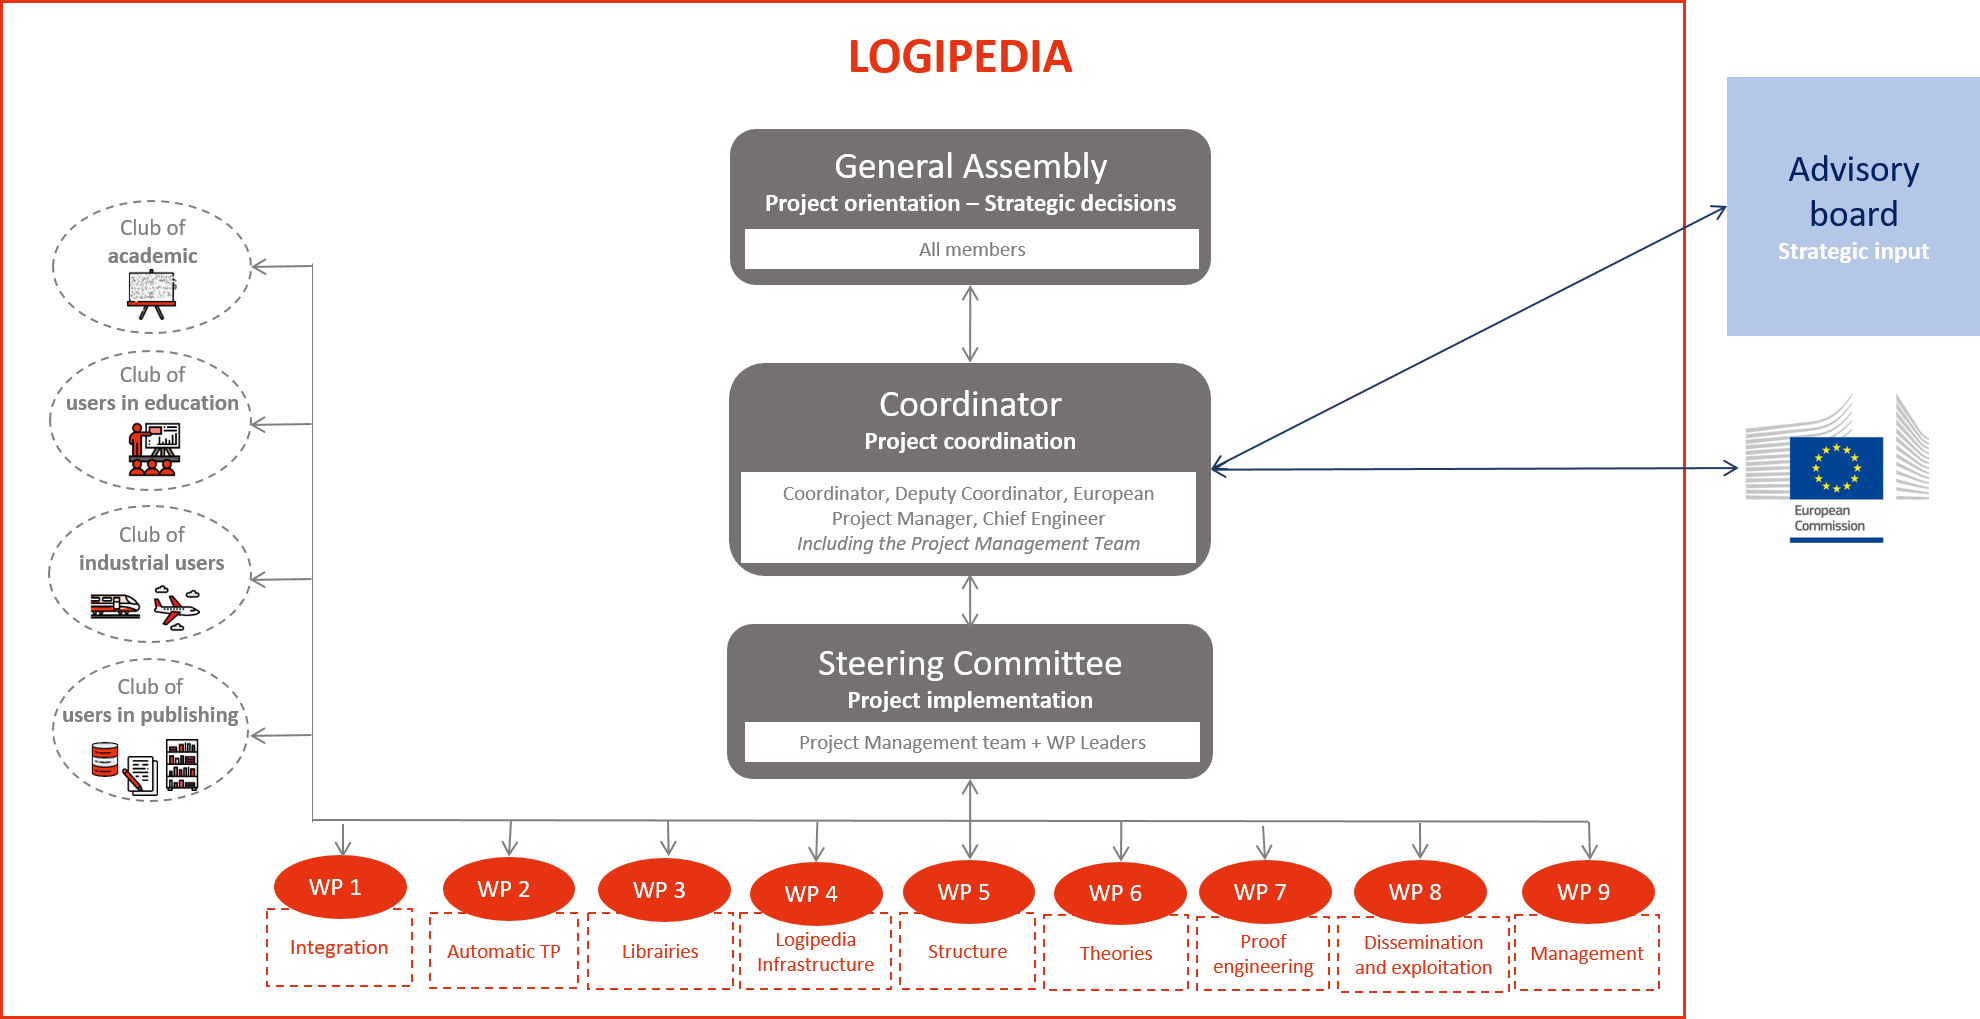
\includegraphics[width=\textwidth]{img/Gouvernance}

In this picture add the EC (talks to Coordinator only)

vice coordinator -> Deputy coordinator

Names of WP

Place of the cooddinator : outside of the bulbe talks to the SN

General assembly talks to SC (and not the SC is part of it)


\subsubsection*{The project management team}

\begin{compactitem}
\item{\bf The Coordinator}: the 
coordinator is responsible for the coordination of
scientific and technical activities in order to meet the objectives
set by the European Commission in the Grant Agreement. The 
coordinator works closely with the work package leaders
within the steering committee, in order to monitor the progress of the
scientific and technical work and identify potential risks within each
work package. The coordinator will daily
collaborate with the European project manager in charge of the
day-to-day management of Logipedia. The project will be managed by Pr
Gilles Dowek, permanent senior researcher at Inria Saclay. He will
also chair the meetings of both the general assembly and steering
committee.

\item{\bf The Deputy Coordinator}: The Deputy coordinator, Frédéric
Blanqui, seconds and replaces the coordinator if needed.

\item{\bf The European Project Manager}: The European project manager
  is a team member of the Technology Transfer and Partnership Office
  of Inria Saclay. He or she is in charge of all administrative,
  financial and legal management tasks as listed in
  \WPref{management}. The European project manager is the interface
  between the project and the European Commission as it represents the
  point of contact for the European Commission. The European project
  manager has the overall administrative and financial responsibility
  for the organisation and administrative and financial monitoring of
  the project.

\item{\bf The Chief Engineer}: The chief engineer is an experienced
research engineer from Inria Saclay and is responsible for ensuring
the development and maintenance of tools at Inria Saclay and
supervising the development tasks achieved at the other
beneficiaries. The chief engineer will ensure the coherence of the
Logipedia tools development, according to the defined schedule in the
Grant Agreement.
\end{compactitem}

Innovation management and intellectual property rights issues will be
handled by the European project manager, supported by the experienced
Technology Transfer and Partnerships Office of Inria Saclay. The
project management team will establish appropriate policies and rules
for the management of intellectual property rights for the knowledge
developed within the project, as well as the identification of the
opportunities for the exploitation of the project results in
innovation activities. Issues related to innovation and/or
intellectual property rights management will be tackled at every
steering committee meeting.

\subsubsection*{The operational level}

\begin{compactitem}
\item{\bf The Steering Committee}: The steering committee is composed
  of the Coordinator, the Deputy coordinator, the chief engineer, the
  European project manager and the work package leaders. The steering
  committee is the supervisory body for the implementation of the
  project. The steering committee is responsible innovation,
  intellectual property, and for monitoring the activities of the
  project and the implementation of decisions taken by the general
  assembly. It can formulate proposal for changes in the description
  of action and the related consortium budget. Those changes will have
  to be agreed by the general assembly first and then the European
  commission. The steering committee is chaired by the coordinator.

\item{\bf The Work Package Leaders}: The work package leaders are
responsible for the monitoring and management of the activities and
results within their work packages. In particular, work package
leaders i) identify deviations from the project plan and report them
to the steering committee, ii) manage and supervise the preparation of
reports and their timely delivery, iii) control and monitor activities
of tasks and regularly meet once per month with task leaders, iv)
manage the information flow with other work packages via the steering
committee.

\item{\bf The Task Leaders}: The task leaders are responsible for
coordinating the scientific and technical work in their task and
making the day to day technical decisions that solely affect their
task. Inter-task decisions are coordinated with the work package
leaders.

\item{\bf The Club Leaders}: The club leaders are in charge of
disseminating of the tools developed by the Logipedia consortium in
various communities. They organize the activity of the club. They give
ongoing feedback to the consortium during the course of the project.
\end{compactitem}

\subsubsection*{The strategic level}

\begin{compactitem}
\item{\bf The General Assembly}: The general assembly is composed by all
the members of the consortium, with each representative having one
vote. Every new partner will have a voting right. The general assembly
will gather at least once a year, and as many virtual meetings as
needed. The general assembly is the main governance and ultimate
decision-making body of the consortium. The general assembly must
review the project progress, decide on contingency actions in case of
deviations from the plan and take final decisions on policy and
contractual issues and conflicts as requested by the steering
committee.

\item{\bf The Advisory Board}: The advisory board is a consultation body to
the steering committee and general assembly. It will bring external
and non-legally binding perspective on the scientific and technical
development of the project, ecosystem building and the future of the
encyclopedia. The advisors of this board will attend the yearly
general assembly plenary meeting and will be consulted on the strategy
of the project. The advisory board should aim at representing the
stakeholders of the Logipedia ecosystem without including any
beneficiary or associate partner’s employees. It will be composed of,
among others, industrial and international academic partners
(including non-European ones) apointed by the coordinator after
consulting the steering committee. To start with, we suggest to
include: June Andronick (Data61, Kensington NSW, AU), Denis Cousineau
(Mitsubishi Electric R\&D Centre Europe, FR), Thomas Letan (ANSSI, FR),
Jacques Fleuriot (University of Edinburgh, UK), Natarajan Shankar
(SRI, US), Aaron Stump (Iowa University, US), Laurent Voisin
(Systerel, FR).
\end{compactitem}

\subsubsection*{Internal communication and collaborative ecosystem}

The communication of the consortium including their internal tools is
managed in task 10.2.  The consortium will make use of a number of
project management tools, such as a visio conferencing tool, a project
repository to have an updated account of the project’s important
documents, the progress of the work packages work and deliverables,
all the advances in the project and all the meetings minutes, mailing
lists, etc. that facilitate the smooth execution of the project. This
collaboration environment will be provided by the coordinator of the
project.

Work packages, chaired by work package leaders, will have monthly
planned visio conferences and meetings as need by the work plan;
additional technical meetings may be set up by task leaders or
individual partners. The steering committee will have monthly visio
conferences and will meet twice a year. Dedicated working groups will
be planned as needed according to the work plan.  All meetings will be
documented by minutes listing major decisions and action items.

The project management team will be in charge of all organisational
issues in the general assembly meetings, supported by the local
partner. The project will organise meetings of the general assembly at
least once a year. To equally share travel costs among partners,
physical meetings will be located by rotation at partners’
locations. Project review meetings will be done on a regular basis
according the Grant Agreement provisions.

%%%%%%%%%%%%%%%%%%%%%%%%%%%%%%%%%%%%%%%%%%%%%%%%%%%%%%%%%%%%%%%%%%%%%%%%%%%%%%
\subsection{Decision-making Process}

Our approach for the decision-making process is to locate the decision
as close as possible to the level responsible for the execution (from
task to general assembly level). Decisions are managed within
frequent project meetings, either on-site or via
teleconference. Decisions can be also managed by consultation. If
voting is needed, the agenda should clearly indicate this fact. Quorum
and voting rules will be defined in the Consortium
Agreement. Decisions are binding once the relevant part of the meeting
minutes has been accepted. Any changes to the project plan and scope
must be reviewed and approved by all levels of project management,
before proposing these changes to the steering committee and any
modifications will be considered rejected, after rejection on any of
these involved levels.

Another guiding principle is to avoid conflicts. Nevertheless, should
one arise, a conflict resolution will be ready to be put in place to
deal with it accordingly. The conflict resolution foresees that each
conflict will be mediated, solved or decided at the lowest level
possible. Attempts to solve issues within the consortium will be
carried out in increasing order of authority first at task level
(management of task leader), work package level (management of work
package leaders), and then following the management bodies till the
general assembly. Further rules related to conflict resolutions will
be laid out in the Consortium Agreement.

%%%%%%%%%%%%%%%%%%%%%%%%%%%%%%%%%%%%%%%%%%%%%%%%%%%%%%%%%%%%%%%%%%%%%%%%%%%%%%
\subsection{Monitoring and reporting}

\subsubsection*{Internal reporting}

The project management team continuously monitors the project plan
with its milestones. Each work package leader will be
responsible for the correct execution of the implementation plan for
the corresponding work package. In terms of reporting, this means the work package leaders
will be in charge of gathering the information related to their own
work packages.

Regular audio-conferences of the Steering Committee are foreseen,
which allows work package leaders to identify risks and
discuss them together. This ensures that management (coordination,
European project manager) is aware of potential problems and
deviations and can initiate countermeasures long before a situation
becomes critical. This ensure to spot the blocking points and implements
the solution at the right time.


In case there is a deviation from the work plan, the 
coordinator will initiate corrective actions through the
task leader and the work package leader. The work package leader will
be responsible to implement these actions in dialogue with the
different partners involved in their work packages.

\subsubsection*{Reporting to the European Commission}

The Logipedia consortium will follow the mandatory reporting period
required by the European Commission. 

The project management team will provide the necessary templates in
order to achieve the reporting in due time. Work package leaders will
be asked to gather the relevant information provided by the task
leader regarding their work package and to summarise in order to be
reviewed by the steering committee. It will then be treated by the
coordinator and European project manager and sent to the
European Commission.

%%%%%%%%%%%%%%%%%%%%%%%%%%%%%%%%%%%%%%%%%%%%%%%%%%%%%%%%%%%%%%%%%%%%%%%%%%%%%%
\subsection{Significant risks and associated contingency plans}
\label{sec:risks}

\subsubsection*{Scientific risks}

\begin{longtable}{|p{0.30\textwidth}|p{0.10\textwidth}|p{0.50\textwidth}|}
\hline
{\bf Description of the risk}
&
{\bf Work packages involved}
&
{\bf Proposed measure of mitigation}
\\
\hline
Some theories are difficult to express in Dedukti.
(Probability: medium. Severity: low.)

{\color{red} It is not that it is difficult that is a risk, it is
that we fail to do it}
&
WP6
&
We have carefully divided the systems into two groups: those that do not
present risks (WP1) and those that do (WP6). The success we got with the
theories implemented in systems of the first group gives us confidence
that the theories implemented in those of the second can also be
expressed in Dedukti.  If one of them happens to be more difficult, we
can still build a large encyclopedia with the systems of the first
group. We can also extend Dedukti so that it can express more theories,
as we have already done in the past.
\\
\hline
Some libraries require too much time and memory
to be expressed in Dedukti (Probability: medium. Severity: low.)
&
WP3
&
There are several ways to mitigate this risk: optimize the
representation of data (sharing, elimination of redundancies, etc.), 
use faster and larger computers. This may also mean that some tasks
of this work package are premature and that we have to wait for
faster computers, that Moore's law will provide.
\\
\hline
No adoption from the community. (Probability: low. Severity: high.)
&
All 
&
The community may fail to adopt Logipedia for several reasons. Because
of a problem of design of Logipedia, in which case we will have to
understand what needs to be changed in a second version.  It may be
because the Logipedia community is too small.  This explains that we
have decided to include twenty-eight partners in the project.  It may
also be because of an insufficient dissemination activity.  This is
why we propose to create the four clubs of users and we will devote
time and energy to the animation of these clubs, together with other
dissemination activities, such as summer schools and conferences.
\\
\hline
\end{longtable}

\subsubsection*{Management risks}

\begin{longtable}{|p{0.30\textwidth}|p{0.10\textwidth}|p{0.50\textwidth}|}
\hline
Brexit disrupts the project (Probability: low. Severity: medium.)
&
All (specially WP6, WP7)
&
As we have two partners from the United Kingdom, Brexit could be a risk
for our project. Yet, we are quite confident
that scientific
cooperation will continue after Brexit and that the British partners
of the project will continue to be part of it.
As this project is submitted during H2020 and nothing changes until
the end of 2020, Logipedia is safe for the start of the project. From
2021 onwards, we can hope some agreement will be concluded as the UK
already made public its willingness to maintain collaborations.
If it were not the
case, we would have to reallocate the impacted tasks to other partners. 
\\
\hline
One partner leaves (Probability: low. Severity: depends on the partner.)
&
All
&
The impact of such a default of one partner of course depends on the
partner. But, during the preparation of this project, we have been
careful to develop an atmosphere of trust and solidarity between the
partners. If this happened
we would need to adapt the objectives of the work package the partner
was supposed to contribute to.
\\
\hline
Difficulty to find people (doctoral students, post-docs, engineers, etc.)
(Probability: medium. Severity: low.)
&
All
&
This project will require hiring a fair number of people. This may be
difficult in some European countries. If this happens we will use the
size of the network to find candidates in other countries to meet
the objectives of the project.\\
\hline
\end{longtable}

%%%%%%%%%%%%%%%%%%%%%%%%%%%%%%%%%%%%%%%%%%%%%%%%%%%%%%%%%%%%%%%%%%%%%%%%%%%%%%
\subsection{Milestones}\label{sec:milestones}

{\color{red} Bad idea, to have all milestones < 24}


As show by the Pert diagram above, two work packages, are critical, as
many others depend on them: work package 4 ``Access to the
encyclopedia'' that is focused on the development of the
infrastructure itself and work package 1 ``Integration'' that focuses
on populating this infrastructure with theories and proofs. All work
packages depend on work package 4, and work packages 3 ``Large
libraries'', work package 5 ``Structure of the encyclopedia'', and
work package 7 ``Proof engineering'' depend on work package 1.
As a consequence our milestones are completions of the key tasks of
work packages 4 and 1.

All milestones have to be completed in the first and second year
of the project, which is a sign of controllability of the project.
No milestone is the completion of a
task of the two, more risky, joint research activity work packages:
work package 6 ``Theories'' and work package 7 ``Proof engineering'',
which is a sign of robustness of the project.
  

%\begin{longtable}{|p{0.1\textwidth}|p{0.55\textwidth}|p{0.2\textwidth}|p{0.1\textwidth}|}
%%%%%%%%%%%%%%%%%%%%%%%%%%%%%%%%%%%%%%%%%%%%%%%%%%%%%%%%%%%%%%%%%%%%%%%%%%%%%%
%\hline
%1
%&
%Prototype version of Logipedia platform
%&
%deliverable D4.7
%&
%M 14
%\\
%\hline
%2
%&
%Opam for Logipedia
%&
%deliverable D4.3
%&
%M 20
%\\
%\hline
%\end{longtable}

%\begin{longtable}{|p{0.1\textwidth}|p{0.55\textwidth}|p{0.2\textwidth}|p{0.1\textwidth}|}
%%%%%%%%%%%%%%%%%%%%%%%%%%%%%%%%%%%%%%%%%%%%%%%%%%%%%%%%%%%%%%%%%%%%%%%%%%%%%%
%\hline
%3
%&
%Instrumentation of Isabelle 
%&
%deliverable D1.2
%&
%M 12
%\\
%\hline
%4
%&
%Instrumentation of HOL4 
%&
%deliverable D1.3
%&
%M 12
%\\
%\hline
%5
%&
%Instrumentation of Coq 
%&
%deliverable D1.6
%&
%M 8
%\\
%\hline
%\end{longtable}

{\color{red} order the milestones by date}

  
\begin{milestones}
\milestone[id=platform,verif=Inspection,month=14]
  {Prototype version of the Logipedia platform}
  {Release of a first version of the Logipedia platform}
\milestone[id=opam,verif=Inspection,month=20]
   {Opam for Logipedia}
   {Release of a first version of Opam for Logipedia}
\milestone[id=isabelle,verif=Inspection,month=12]
   {Instrumentation of Isabelle}
   {Integration of the Isabelle standard library in Logipedia}
\milestone[id=hol4,verif=Inspection,month=12]
   {Instrumentation of HOL4}
   {Integration of the HOL4 standard library in Logipedia}
\milestone[id=coq,verif=Inspection,month=8]
   {Instrumentation of Coq}
   {Integration of the Coq standard library in Logipedia}
\end{milestones}

{\


%%% Local Variables:
%%%   mode: latex
%%%   mode: flyspell
%%%   ispell-local-dictionary: "english"
%%% End:


\section{The {\protect\pn} consortium as a whole}\label{sec:consortium}
\begin{todo}{from the proposal template}
  Describe how the participants collectively constitute a consortium capable of achieving
  the project objectives, and how they are suited and are committed to the tasks assigned
  to them. Show the complementarity between participants. Explain how the composition of
  the consortium is well-balanced in relation to the objectives of the project.  

  If appropriate describe the industrial/commercial involvement to ensure exploitation of
  the results. Show how the opportunity of involving SMEs has been addressed
\end{todo}

The project partners of the \pn project have a long history of successful collaboration;
Figure~\ref{tab:collaboration} gives an overview over joint projects (including proposals) and
joint publications (only international, peer reviewed ones).

\jointorga{Fau,Bol}% CICM
\jointorga{Inn,Bol}% CICM
\jointpub{Fau,Bol}% CICM paper
\jointpub{Tum,Bol}% CICM paper
\jointpub{Fau,TUM}% 
%\jointsup{Fau,}
\jointsoft{Fau,Tum}% Isabelle Extension
\jointsoft{Fau,Bol}% Coq exporter
\jointpub{Inr,Bol}% ELPI
\jointproj{Inr,Bol}% MoWGLI
\coherencetable

\subsection{Subcontracting}\label{sec:subcontracting}
\begin{todo}{from the proposal template}
  If any part of the work is to be sub-contracted by the participant responsible for it,
  describe the work involved and explain why a sub-contract approach has been chosen for
  it.
\end{todo}

\ednote{@Rabe: justify subcontracting for Wenzel}

\subsection{Other Countries}\label{sec:other-countries}
\begin{todo}{from the proposal template}
  If a one or more of the participants requesting EU funding is based outside of the EU
  Member states, Associated countries and the list of International Cooperation Partner
  Countries\footnote{See CORDIS web-site, and annex 1 of the work programme.}, explain in
  terms of the project’s objectives why such funding would be essential.
\end{todo}

\subsection{Additional Partners}\label{sec:assoc-partner}
\begin{todo}{from the proposal template}
  If there are as-yet-unidentified participants in the project, the expected competences,
  the role of the potential participants and their integration into the running project
  should be described
\end{todo}

%%% Local Variables:
%%% mode: latex
%%% TeX-master: "propB"
%%% End:


\section{Resources to be Committed}\label{sec:resources}
\begin{todo}{from the proposal template}
Maximum length: two pages

Describe how the totality of the necessary resources will be mobilized, including any resources that
will complement the EC contribution. Show how the resources will be integrated in a coherent way,
and show how the overall financial plan for the project is adequate.

In addition to the costs indicated on form A3 of the proposal, and the effort shown in Section 1.3
above, please identify any other major costs (e.g. equipment). Ensure that the figures stated in Part B
are consistent with these.
\end{todo}

\subsection{Travel Costs and Consumables}\label{sec:travel-costs}
\subsection{Subcontracting Costs}
\subsection{Other Costs}

%%% Local Variables: 
%%% mode: LaTeX
%%% TeX-master: "propB"
%%% End: 

% LocalWords:  pn newpage site-FAU site-efo site-baz jointpub efo baz
% LocalWords:  jointproj coherencetable assoc-partner

\newpage
\renewcommand\addcontentsline[3]{}
\section{Individual Participants}\label{sec:partners}
\begin{todo}{from the proposal template}
For each participant in the proposed project, provide a brief description of the legal entity, the main
tasks they have been attributed, and the previous experience relevant to those tasks. Provide also a
short profile of the individuals who will be undertaking the work.\\
Maximum length for Section 2.2: one page per participant. However, where two or more departments within
an organisation have quite distinct roles within the proposal, one page per department is acceptable.\\
The maximum length applying to a legal entity composed of several members, each of which is a separate
legal entity (for example an EEIG1), is one page per member, provided that the members have quite distinct
roles within the proposal.
\end{todo}
\newpage
\begin{sitedescription}{Bel}

\paragraph{Organization:}
\ednote{Give a one-paragraph run-down of the site and the team there. }

\paragraph{Main tasks:}

\begin{compactitem}
\item\ednote{specify the main tasks and reference the respective work packages} 
\end{compactitem}


\paragraph{Relevant previous experience:}

\ednote{give an overview over previous work and projects that add to the \pn project}

\paragraph{Specific expertise:}

\begin{compactitem}
\item \ednote{give three to five specific areas of expertise that pertain to the \pn project}
\end{compactitem}

\paragraph{Staff members undertaking the work:}

\textbf{Dr.\ Great Leader}\ednote{describe the site leader and his expertise}
\textbf{Joe Implementor}\ednote{and more of them. }
\ednote{provide the key publications below}
\keypubs{providemore}


Predrag Janičić, Filip Marić, Vesna Marinković, Danijela Simić, Sana Stojanović-Đurđević





\end{sitedescription}
%%% Local Variables: 
%%% mode: latex
%%% TeX-master: "../propB"
%%% End: 

% LocalWords:  site-jacu.tex clange sitedescription emph compactitem pn semmath
% LocalWords:  prosuming-flexiformal KohSuc asemf06 GinJucAnc alsaacl09 StaKoh
% LocalWords:  tlcspx10 KohDavGin psewads11 ednote Radboud Bia ystok CALCULEMUS
% LocalWords:  textbf keypubs OntoLangMathSemWeb uwb Deyan Ginev Stamerjohanns
% LocalWords:  searchability
\newpage
\begin{sitedescription}{Bia}

\paragraph{Organization:}

The University of Bialystok (UwB) was established in 1997 from a~branch of Warsaw University after 29 years of its existence.
Today UwB is one of the largest and strongest academic centers in North-Eastern Poland.
It consists of nine faculties (including one located in Vilnius, Lithuania) and five institutes.
Classes and lectures are delivered by approx. 850 academic teachers (nearly 200 are independent research scholars).
At present UwB educates over 8000 students in almost 30 fields of study.

The Mizar research group at UwB has several decades of experience in designing formal languages for efficient encoding of mathematical data and implementing formal proof-checking software. The group coordinates the development of the Mizar Mathematical Library (MML) -- a~large centralized collection of formalized mathematical definitions, theorems and their proofs authored by over 260 contributors from 20 countries. The library is maintained and distributed in a~variety of data formats, including interactive web-based documents and automatically generated natural language journal articles. The members of the group have participated in a~number of EU funded research
and collaboration projects,
as well as the EUTYPES Cost Action. The Mizar group has also organized the MKM 2004 and CICM 2016 conferences.

\paragraph{Main tasks:}

\begin{compactitem}
\item Expressing the foundations of the Mizar logic in Dedukti \WPref{theories}
\item Extracting in-depth knowledge from the Mizar proofs \WPref{theories}
\item Developing Dedukti techniques corresponding to Mizar proof checking \WPref{theories}
\end{compactitem}

\paragraph{Relevant previous experience:}

The Mizar research group has carried out several grants within European Union Framework Projects and also funded by Polish National Science Center and Office of Naval Research, US.
The most related to the project are:

\begin{compactitem}
\item ``Isabelle Emulator for Mizar: Environment for Mizar Mathematical Library Re-verification'', funded by Polish National Science Center, project manager: Karol Pąk, 7/2016--7/2019
\item ``Independent Verification of Mizar Logic'', funded by the OeAD Scientific \& Technological Cooperation with Poland, project coordinator at the Polish side: Karol Pąk, 5/2016--4/2018
\item ``Algorithms Concerning the Legibility of Natural Deduction Proofs'', funded by Polish National Science Center, project manager: Karol Pąk, 7/2013--1/2017
\item ``Management of a~Large Repository of Computer Verified Mathematical Knowledge'', funded by Polish Ministry of Science and Higher Education, project manager: Andrzej Trybulec, 5/2009--5/2012
\item ``Types for Proofs and Programs'', TYPES II EU FP6 510996, site of the project coordinated by Chalmers, 9/2004--8/2007
\end{compactitem}

\paragraph{Specific expertise:}

\begin{compactitem}
\item Expressing and translating formal semantics
\item Experience with Mizar kernel augmentation for proof object extraction
\item In-depth knowledge of the Mizar foundations
\item Managing large mathematical repositories
% Wg mnie Nie mają się do projektu.
% \item Computer-aided formalization and verification of mathematics
%\item Designing formal languages
\end{compactitem}

\paragraph{Staff members undertaking the work:}

\begin{compactitem}

\item\textbf{Dr.\ Artur Korniłowicz} is the deputy director for science and head of the Department of Programming and Formal Methods
at the Institute of Informatics at the University of Bialystok.
Korniłowicz received his PhD in computer science from Shinshu University, Nagano, Japan in 2001.
In 2017 he received habilitation from the University of Warsaw, Poland.
Korniłowicz's main research interests are in formal verification of mathematics and verification of algorithms.
He is one of the key developers of the Mizar proof-assistant and the author of over 100 Mizar formalizations.
In 2005 he was awarded {\'S}leszy\'nski Prize for Formalization of the Jordan Curve Theorem.
In the period 7/2001--6/2002 Korniłowicz was a~CALCULEMUS postdoctoral fellow at the Istituto per la Ricerca Scientifica e~Tecnologica, Trento, Italy under the CALCULEMUS project within EU FP5;
and in the period 7/2003--3/2005 he was a~Japan Society for the Promotion of Science postdoctoral fellow at the Shinshu University, Nagano, Japan.

\item\textbf{Dr.\ Czesław Byliński} is head of the Computer Networks Section at the University of Bialystok.
He received his PhD in computer science from Shinshu University, Japan in 1998.
Since 1978 he has been a~member of the Mizar Project.
He participates in the implementation of the Mizar language and the developing the Mizar system tools. 
Since 2014, he has been in charge of the Mizar implementation team.

\item\textbf{Dr.\ Adam Grabowski} is an adjunct at UwB since 2006, 
with a~focus on the formalization of mathematics and computer science.
He received his PhD in mathematics from the University of Silesia in Katowice, Poland in 2005 
and PhD in computer science from Shinshu University, Nagano, Japan in 2005.
Currently, he works on the application of automated proof assistants
in the modeling of the reasoning under uncertainty: fuzzy and rough sets.
He has authored over 120 papers in refereed journals and international conference
proceedings, including over 70 formalizations in Mizar.
He received twice the {\'S}leszy\'nski Award (1998, 2000) granted by the Association of Mizar Users.
Since 1999 he has been the head of the Library Committee of Association of Mizar Users, taking care of
the management and development of the Mizar Mathematical Library.

\item\textbf{Dr.\ Adam Naumowicz} is a~member of the core Mizar development team. 
With his background in mathematics and linguistics, he received his PhD in computer science in 2005
for research on formalizing recent mathematical results. His recent works focus on extending Mizar checker's computational power, 
interacting with external tools and developing web-based services. 
He's been elected twice to serve as Mathematical Knowledge Management representative to the Steering Committee
of Conference on Intelligent Computer Mathematics (CICM).
He was also the main organizer of CICM 2016 held at the University of Bialystok. 
He acts as Poland's representative in the Management Committee of the European research network on types for programming and verification (Cost Action EUTypes).

\item\textbf{Dr.\ Karol Pąk} has developed the Isabelle/Mizar system where
he specified Mizar in the Isabelle logical framework
giving the complete semantics of the system, including
the underlying first-order logic variant, soft type system, and definitional mechanisms.
Additionally, he proposed a semi-automatic translation of several MML articles
to the resulting object logic to cross-verify them.
Furthermore he has been developing methods
that automatically improve readability of natural deduction proofs
by the step order manipulation as well as lemma extraction.

\end{compactitem}

\paragraph{Publications:}

\begin{compactitem}

\item Bancerek, G., Byliński, C., Grabowski, A., Korniłowicz, A., Matuszewski, R., Naumowicz, A., Pąk, K.:
``The role of the {M}izar {M}athematical {L}ibrary for interactive proof development in {M}izar''.
Journal of Automated Reasoning \textbf{61}(1), 9--32 (2018).
\\\url{https://doi.org/10.1007/s10817-017-9440-6}

\item Bancerek, G., Byliński, C., Grabowski, A., Korniłowicz, A., Matuszewski, R., Naumowicz, A., Pąk, K., Urban, J.:
``Mizar: State-of-the-art and Beyond''.
Intelligent Computer Mathematics, International Conference, CICM 2015, Washington, DC, USA, July 13--17, 2015, Proceedings., (M. Kerber, J. Carette, C. Kaliszyk, F. Rabe, V. Sorge Ed(s).), Lecture Notes in Comput. Sci. vol. 9150, Springer, Berlin, 2015, pp. 261--279.
\\\url{https://doi.org/10.1007/978-3-319-20615-8_17}

\item Kaliszyk, C. Pąk, K.: ``Semantics of Mizar as an Isabelle Object Logic''.
Journal of Automated Reasoning \textbf{63}(3), 557--595 (2019).
\\\url{https://doi.org/10.1007/s10817-018-9479-z}

\item Kaliszyk, C. Pąk, K.: ``Scalable Declarative Proof Translation'',
Tenth International Conference, Interactive Theorem Proving, ITP 2019, Portland,
OR, USA. Proceedings,  LIPIcs, Vol. 141, 35:1--35:7 (2019).
\\\url{https://doi.org/10.4230/LIPIcs.ITP.2019.35}

\item Brown, C.E., Kaliszyk, C., Pąk, K.: ``Higher-order Tarski Grothendieck as a~Foundation for Formal Proof'',
Tenth International Conference, Interactive Theorem Proving, ITP 2019, Portland,
OR, USA. Proceedings,  LIPIcs, Vol. 141, 9:1--9:16 (2019).
\\\url{https://doi.org/10.4230/LIPIcs.ITP.2019.9}

\end{compactitem}

\end{sitedescription}

%%% Local Variables:
%%% mode: latex
%%% TeX-master: "../propB"
%%% End:

% LocalWords:  site-jacu.tex clange sitedescription emph compactitem pn semmath
% LocalWords:  prosuming-flexiformal KohSuc asemf06 GinJucAnc alsaacl09 StaKoh
% LocalWords:  tlcspx10 KohDavGin psewads11 ednote Radboud Bia ystok CALCULEMUS
% LocalWords:  textbf keypubs OntoLangMathSemWeb uwb Deyan Ginev Stamerjohanns
% LocalWords:  searchability
\newpage
\begin{sitedescription}{Bol}

\logo{Bologna}

Founded in 1088, the Alma Mater Studiorum – Università di Bologna (UNIBO) is known as the oldest University of the western world. Nowadays, UNIBO still remains one of the most important institutions of higher education across Europe and the second largest university in Italy. UNIBO is organized in a multicampus structure with 5 operating sites and, since 1998, also a permanent headquarters in Buenos Aires: 11 Schools, 33 Departments, 12 Research and Innovation Centers and more than 84.000 students. The Alma Mater has already been partner or coordinator of more than 244 EU projects in the Horizon 2020 program, for a grand total of more than 100,000,000 euros.

The activity of the University of Bologna are conducted within the Department of Computer Science and Engineering (DISI), which is one of the top Computer Science and Engineering departments in Italy, offering a broad spectrum of expertise ranging from theoretical computer science to software, hardware and application design and development. DISI is currently member or coordinator of 12 on-going EU projects.

The research group that will be in charge of Logipedia at UNIBO is leaded by Dr. Claudio Sacerdoti Coen. The group is active in the areas of formal methods, interactive theorem proving and mathematical knowledge management, which are all relevant to the project.

\paragraph{Main tasks:}

\begin{compactitem}
\item \WPref{instrumentation}, task \taskref{instrumentation}{matita}: Integrate the Matita translator in Matita itself (Asperti, Post-Doc)
\item \WPref{instrumentation}, task \taskref{instrumentation}{coq}: Instrument Coq (Sacerdoti Coen, Post-Doc)
\item \WPref{structuring}, task \taskref{structuring}{strontorepml}: Ontological Representation of Formal Libraries (Asperti, Sacerdoti Coen, Post-Doc)
\item \WPref{alignment}, task \taskref{alignment}{alignservices}: Alignment-Based Services (Sacerdoti Coen, Post-Doc)
\end{compactitem}

\paragraph{Publications, products or services:}

\begin{compactitem}
\item F. Guidi, C. Sacerdoti Coen, E. Tassi:
Implementing type theory in higher order constraint logic programming. Mathematical Structures in Computer Science 29(8): 1125-1150 (2019)
\item A. Condoluci, M. Kohlhase, D. Müller, F. Rabe, C. Sacerdoti Coen, M. Wenzel: Relational Data Across Mathematical Libraries. CICM 2019: 61-76
\item C. Dunchev, F. Guidi, C. Sacerdoti Coen, E. Tassi:
ELPI: Fast, Embeddable, $\lambda$Prolog Interpreter. LPAR 2015: 460-468
\item A. Asperti, C. Sacerdoti Coen, E. Tassi, S. Zacchiroli:
User Interaction with the Matita Proof Assistant. J. Autom. Reasoning 39(2): 109-139 (2007)
\item A. Asperti, F. Guidi, C. Sacerdoti Coen, E. Tassi, S. Zacchiroli:
A Content Based Mathematical Search Engine: Whelp. TYPES 2004: 17-32
\end{compactitem}

\paragraph{Previous projects or activities:}

Members of the group have expertise in the fields of Mathematical Knowledge Management and Interactive Theorem Proving, notably designing and implementing of theorem provers and building (web-)services for mathematical libraries.
They have been part of several national and international projects, including

\begin{compactitem}
\item FET-Open EU Project MoWGLI (Math on the Web: Get it by Logic and Interfaces). The project was focused on making the library of the Coq prover easily accessible outside the system and on the Web. MoWGLI explored independent verification, indexing, search and retrieval and transformation of proofs coming from Coq. All the previous services were implemented as web services using W3C technologies. Logipedia is more ambitious in aiming at providing the same services but for every system at once. They by-product of MoWGLI was the creation of the interactive theorem prover Matita.

\item FET-Open EU Project CerCo (Certified Complexity). The project focused on formal proofs applied to formal methods in the domain of real time systems and complexity preserving compilation. The main technical tool employed was Matita.

\item IST-2001-37057 MKMNET, the COST Action EUTypes and a number of previous succesfull European projects on Mathematical Knowledge Management and on Type Theory.
\end{compactitem}

\paragraph{Infrastructures or technical equipments:}

\begin{compactitem}
\item The ELPI Higher Order Constraint Logic Programming language, co-developed with INRIA, a general purpose programming language that doubles as a domain specific language for the manipulation of logical and mathematical expressions and for the implementation of proof transformations.
\item The interactive theorem prover Matita
\item Web services developed in the MoWGLI EU project to provide access on the Web to Coq proofs, with indexing and searching capabilities.
\end{compactitem}

\paragraph{Persons primarily responsible for carrying out the proposed activities:}

\begin{itemize}
\item \textbf{Claudio Sacerdoti Coen Leader} is associate professor of computer science since 2015. He published more than 15 journal papers and 50 conference papers on Mathematical Knowledge Management, Interactive Theorem Proving and the theory of lambda-calculus. The most recent project he coordinated was the EU FET Open Project CerCo (Certified Complexity). He was also work-package leader for the EU FET Open Project MoWGLI (Math on the Web, Get it by Logic and Interfaces). He is one of the main developers of Matita and co-developer of the ELPI language.

\item \textbf{Andrea Asperti} is full professor of computer science at the University of Bologna, one of the founders of the Mathematical Knowledge Management discipline and the previous coordinator of the HELM project that lead to the development of Matita. Before becoming an expert in interactive theorem proving he worked on category theory, lambda-calculus and linear logic. His current research interests also cover machine learning.
\end{itemize}

\end{sitedescription}
%%% Local Variables: 
%%% mode: latex
%%% TeX-master: "../propB"
%%% End: 

% LocalWords:  site-jacu.tex clange sitedescription emph compactitem pn semmath
% LocalWords:  prosuming-flexiformal KohSuc asemf06 GinJucAnc alsaacl09 StaKoh
% LocalWords:  tlcspx10 KohDavGin psewads11 ednote Radboud Bia ystok CALCULEMUS
% LocalWords:  textbf keypubs OntoLangMathSemWeb uwb Deyan Ginev Stamerjohanns
% LocalWords:  searchability
\newpage
\begin{sitedescription}{Cle}

\paragraph{Organization:}
\ednote{Give a one-paragraph run-down of the site and the team there. }

\paragraph{Main tasks:}

\begin{compactitem}
\item\ednote{specify the main tasks and reference the respective work packages} 
\end{compactitem}


\paragraph{Relevant previous experience:}

\ednote{give an overview over previous work and projects that add to the \pn project}

\paragraph{Specific expertise:}

\begin{compactitem}
\item \ednote{give three to five specific areas of expertise that pertain to the \pn project}
\end{compactitem}

\paragraph{Staff members undertaking the work:}

\textbf{Dr.\ Great Leader}\ednote{describe the site leader and his expertise}
\textbf{Joe Implementor}\ednote{and more of them. }
\ednote{provide the key publications below}
\keypubs{providemore}
\end{sitedescription}
%%% Local Variables: 
%%% mode: latex
%%% TeX-master: "../propB"
%%% End: 

% LocalWords:  site-jacu.tex clange sitedescription emph compactitem pn semmath
% LocalWords:  prosuming-flexiformal KohSuc asemf06 GinJucAnc alsaacl09 StaKoh
% LocalWords:  tlcspx10 KohDavGin psewads11 ednote Radboud Bia ystok CALCULEMUS
% LocalWords:  textbf keypubs OntoLangMathSemWeb uwb Deyan Ginev Stamerjohanns
% LocalWords:  searchability
\newpage
\begin{sitedescription}{Del}

\logo{TUDelft}

The Programming Languages Research Group at TU Delft is an
internationally leading research group in programming languages, and
active in areas such as language engineering, language design,
domain-specific languages, software verification, and programme logics.
Specifically, Dr. Jesper Cockx is an expert on the Agda system.

\paragraph{Main tasks:}

\begin{compactitem}
  \item \WPref{instrumentation}, task \taskref{instrumentation}{agda}:
  Encoding of features that rely on type-directed conversion -- such
  as eta-equality and definitional irrelevance -- in Dedukti (which
  does not have type-directed conversion).
  \item \WPref{instrumentation}, task \taskref{instrumentation}{agda}:
  Investigating possible designs for a core language for Agda, in
  order to facilitate the exporting of Agda developments to Logipedia.
  \item \WPref{instrumentation}, task \taskref{instrumentation}{agda}:
  Improving the current state-of-the-art on dependently typed
  languages with user-defined rewrite rules on areas such as
  confluence and termination checking.
\end{compactitem}

\paragraph{Publications, products or services:}

\begin{itemize}
  \item Jesper Cockx, Dominique Devriese, Frank Piessens. ``Pattern
  matching without K.'' Proceedings of the 19th ACM SIGPLAN
  International Conference on Functional programming, ACM, 2014.
  \item Jesper Cockx, Dominique Devriese, Frank Piessens. ``Unifiers
  as equivalences: proof-relevant unification of dependently typed
  data.'' Proceedings of the 21st ACM SIGPLAN International Conference
  on Functional Programming, ACM, 2016.
  \item Jesper Cockx, Andreas Abel. ``Elaborating dependent
  (co)pattern matching.'' Proceedings of the ACM on Programming
  Languages, 2(ICFP), 2018.
  \item Gaëtan Gilbert, Jesper Cockx, Matthieu Sozeau, Nicolas
  Tabareau. ``Definitional proof-irrelevance without K.'' Proceedings
  of the ACM on Programming Languages, 3, 2019.
\end{itemize}

%\keypubs{DBLP:conf/icfp/CockxDP14,DBLP:conf/icfp/CockxDP16,DBLP:journals/pacmpl/CockxA18}

\paragraph{Previous projects or activities:}

\paragraph{Infrastructures or technical equipments:}

\paragraph{Persons primarily responsible for carrying out the proposed activities:}

\begin{itemize}

  \item{\bf Jesper Cockx} (leader of work package \WPref{instrumentation}
  and task \taskref{instrumentation}{agda}) is an expert on the theory and
  implementation of Agda, a dependently typed programming language and
  proof assistant that is widely used within the programming languages
  community and beyond. He has worked on both foundational parts of
  Agda such as elaboration of dependent (co)pattern matching and new
  extensions such as rewrite rules and definitional proof
  irrelevance. He is also one of the main contributors to the
  implementation of Agda.

\end{itemize}

% \paragraph{Specific expertise:}

% \begin{compactitem}
% \item Elaboration of high-level programming techniques such as
%   dependent pattern matching to a low-level representation that can be
%   more easily transferred to other languages.
% \item Extending dependently typed languages with user-defined rewrite
%   rules that can be used to encode the theories of other languages.
% \item Automatic translation of Agda developments to Dedukti
%   (collaboration with Guillaume Genestier from Paris-Saclay).
% \end{compactitem}


\end{sitedescription}
%%% Local Variables:
%%% mode: latex
%%% TeX-master: "../propB"
%%% End:

% LocalWords:  site-jacu.tex clange sitedescription emph compactitem pn semmath
% LocalWords:  prosuming-flexiformal KohSuc asemf06 GinJucAnc alsaacl09 StaKoh
% LocalWords:  tlcspx10 KohDavGin psewads11 ednote Radboud Bia ystok CALCULEMUS
% LocalWords:  textbf keypubs OntoLangMathSemWeb uwb Deyan Ginev Stamerjohanns
% LocalWords:  searchability
\newpage
\begin{sitedescription}{Fau}

  \logo{FAU}
  
FAU is the second largest state university in the state Bavaria.
It has 5 faculties, 23 departments/schools, 30 clinical departments, 19 autonomous departments, 656 professors, and about 40\,000 students.

FAU has a strong departments of Computer Science and Mathematics (both 25 Professors) with strong groups in scientific computing, mathematical modeling, and simulation, data management, data visualization, and Pattern recognition.
All of these deal with mathematical data in some way and thus constitute a conducive and supportive environment for \pn.
Importantly the collaborating departments constitute a reservoir of know-how and potential user expertise the \pn project can draw upon for evaluation and testing.

The site leader is Prof. Dr. Michael Kohlhase.
PD Dr. Florian Rabe will be co-PI for the site.

\paragraph*{Main tasks:}

\begin{compactitem}
\item The site co-leads \WPtref{structuring}.
\item The site leads task \tasktref{alignment}{alignsearch}.
\end{compactitem}

\paragraph*{Publications, products or services:}

% a list of up to 5 relevant publications, and/or products, services (including widely-used datasets or software), or other achievements relevant to the call content
The site developed 
\begin{compactitem}
 \item the OMDoc (Open Mathematical Document) format for representing mathematical knowledge \cite{Kohlhase:OMDoc1.2}, which anticipated much of the research proposed here,
 \item the MMT logical framework \cite{RabKoh:WSMSML13} (which uses OMDoc as its representation format), a close relative of Dedukti,
 \item the notion of alignments \cite{GKKMR:alignments:17}, which will be critical in \WPref{alignment},
 \item the comprehensive representation of many major proof assistant libraries (albeit often proof objects) in OMDoc/MMT \cite{KR:oafexp:20},
 \item the MathWebSearch search engine for symbolic formulas knowledge \cite{ProKoh:mwssofse12}.
\end{compactitem}

\paragraph*{Previous projects or activities:}

% a list of up to 5 relevant previous projects or activities, connected to the subject of this proposal

\begin{compactitem}
 \item Prof. Kohlhase and Dr. Rabe were co-PIs of the OpenDreamKit H2020 infrastructure project (2015--2019) on virtual research environments that integrate mathematical computation systems.
 \item Prof. Kohlhase and Dr. Rabe are the PIs of the German-funded OAF project (2014--2020) about representing proof assistant libraries in logical frameworks, specifically the MMT framework.
 \item Prof. Kohlhase co-initiated and organized the three NTCIR community challenges for mathematics information retrieval in 2014/16/17.
 \item Prof. Kohlhase initiated and led the CALCULEMUS! IHP-Research and Training Network.
 \item Prof. Kohlhase participated in the FP6 IST MoWGLI (Mathematics on the Web: Get it by Logic and Interfaces) project.
\end{compactitem}

\paragraph*{Infrastructures or technical equipments:}
% description of any significant infrastructure and/or any major items of technical equipment, relevant to the proposed work

\begin{compactitem}
\item The site hosts http://mathhub.info, a portal for formalized mathematics, mathematical databases, and active mathematical documents.
It hosts about 10GB of data (Theorem Prover Libraries, OEIS, semantic course materials and a multilingual mathematical glossary), serves it via the MMT system and a lightweight browser-based front-end, and includes services like 2D/3D theory graph visualization of the modular structure.
\end{compactitem}

\paragraph*{Persons primarily responsible for carrying out the proposed activities:}

\begin{compactitem}
\item\textbf{Michael Kohlhase} holds the \emph{Professorship for Knowledge Representation and Management} in the Computer Science Department.
The \href{http://kwarc.info}{KWARC} (KnoWledge Adaptation and Reasoning for Content) Group headed by him specializes in knowledge management for Science, Technology, Engineering, and Mathematics (STEM), focusing on the last as a test subject.
Formal logic, natural language semantics, and semantic web technology provide the foundations for the research of the group.
Its group working on \pn will be composed of the following non-exhaustive list: Prof. Dr. Michael Kohlhase, Dr. Florian Rabe, Tom Wiesing, Dennis M\"uller, Jonas Betzendahl and Jan Frederik Schaefer.

\item\textbf{Florian Rabe} obtained his PhD in 2008 and his habilitation in 2014 and is now Akad. Oberrat and Privatdozent in the KWARC group.
Within the group, Kohlhase and Rabe co-advise most students and have shared the administration of research projects for 10 years.
He is an expert in the design, implementation, and evaluation of representation languages for mathematical knowledge and meta-logical frameworks.
He currently chairs the steering committee of \emph{Logical Frameworks and Meta-Languages: Theory and Practice}.
He is the main developer of the MMT language and system and the LATIN logic atlas and has designed and overseen the representation of proof assistant libraries in the OAF project.
\end{compactitem}

\end{sitedescription}

%%% Local Variables: 
%%% mode: LaTeX
%%% TeX-master: "../propB"
%%% End: 
\newpage
\begin{sitedescription}{GU}

\paragraph{Organization:}
\ednote{Give a one-paragraph run-down of the site and the team there. }

\paragraph{Main tasks:}

\begin{compactitem}
\item\ednote{specify the main tasks and reference the respective work packages} 
\end{compactitem}


\paragraph{Relevant previous experience:}

\ednote{give an overview over previous work and projects that add to the \pn project}

\paragraph{Specific expertise:}

\begin{compactitem}
\item \ednote{give three to five specific areas of expertise that pertain to the \pn project}
\end{compactitem}

\paragraph{Staff members undertaking the work:}

\textbf{Dr.\ Great Leader}\ednote{describe the site leader and his expertise}
\textbf{Joe Implementor}\ednote{and more of them. }
\ednote{provide the key publications below}
\keypubs{providemore}
\end{sitedescription}
%%% Local Variables: 
%%% mode: latex
%%% TeX-master: "../propB"
%%% End: 

% LocalWords:  site-jacu.tex clange sitedescription emph compactitem pn semmath
% LocalWords:  prosuming-flexiformal KohSuc asemf06 GinJucAnc alsaacl09 StaKoh
% LocalWords:  tlcspx10 KohDavGin psewads11 ednote Radboud Bia ystok CALCULEMUS
% LocalWords:  textbf keypubs OntoLangMathSemWeb uwb Deyan Ginev Stamerjohanns
% LocalWords:  searchability
\newpage
\begin{sitedescription}{Inn}

\paragraph{Organization:}
The University of Innsbruck is a global Top-200 university and the second
largest university in Austria. UIBK has been involved in a number of FWF
projects related to formal proof, and a large number of national and
international projects including dozens of projects as part of FP5,
FP6, FP7, and H2020.

The research of the Computational Logic group is concerned with the logical
foundations of computer science and their application to the analysis and
verification of complex systems. The group has developed the IsaFoR library,
the largest formalisation of rewriting with more than 5000 theorems. Various
hammer systems developed in the group are today strongest automation techniques
for various formalizations including the Flyspeck project.

\paragraph{Main tasks:}

\begin{compactitem}
\item Collaboration on task ..., the specification of Mizar in Dedukti
\item Dedukti-internal proof automation
\item Alignments
\end{compactitem}

\paragraph{Relevant previous experience:}

\ednote{give an overview over previous work and projects that add to the \pn project}

\paragraph{Specific expertise:}

\begin{compactitem}
\item \ednote{give three to five specific areas of expertise that pertain to the \pn project}
\end{compactitem}

\paragraph{Staff members undertaking the work:}

\textbf{Assoc. Prof. Dr.\ Cezary Kaliszyk} has been working on making proof assistants
more accessible by developing proof automation, proof advice, and other packages for formal
proofs. He has worked on the Isabelle/Mizar object logic, where features of Mizar were
expressed in a logical framework. Kaliszyk has also worked on machine learning for interactive
proofs and has co-organized the AITP conference on the topic in the last few years (AITP). He
has developed multiple hammer systems for higher-order logic and intuitionistic type theory.
Kaliszyk has also worked on alignments between formal systems and between informal and formal
mathematics.

% Postdoc and PhD students that unfortunately will end likely in 2021: Joshua Chen, Miroslav Olšák, Stanisław Purgał

\end{sitedescription}
%%% Local Variables: 
%%% mode: latex
%%% TeX-master: "../propB"
%%% End: 

% LocalWords:  site-jacu.tex clange sitedescription emph compactitem pn semmath
% LocalWords:  prosuming-flexiformal KohSuc asemf06 GinJucAnc alsaacl09 StaKoh
% LocalWords:  tlcspx10 KohDavGin psewads11 ednote Radboud Bia ystok CALCULEMUS
% LocalWords:  textbf keypubs OntoLangMathSemWeb uwb Deyan Ginev Stamerjohanns
% LocalWords:  searchability
\newpage
\begin{sitedescription}{Lmu}

\newcommand\inquotes[1]{``#1''}

\logo{LMU}

Ludwig-Maximilians-Universit\"at (LMU) is a public research university
located in M\"unchen, Germany.  LMU consists of 18 faculties which
accommodate various departments and institutes including the
Mathematisches Institut, where the research group of mathematical
logic is headed by Prof.\ Dr.\ Helmut Schwichtenberg.  The research
areas of the group are such as proof theory, realisability
interpretation, programme extraction, constructive analysis,
constructive algebra, and proof assistant.  In particular in the
research area of proof assistant, the logic group has been actively
developing the Minlog system since early 1990's.

\paragraph*{Main tasks:}

\begin{compactitem}
  \item Encoding the underlying theory of Minlog in Dedukti. \WPtref{theories} \taskref{theories}{minlog}
  \item Implementing the encoder, so that Minlog's libraries and formal proofs of constructive analysis is available in Dedukti with proof checking.
The Logipedia integration level of Minlog is increased to 3 from 0. \WPtref{theories} \taskref{theories}{minlog}
  \item Making Minlog's classical extraction available within Dedukti.  Alignment for concepts in constructive analysis, in particular (co)induction/(co)recursion and predicativity. \WPtref{alignment} \taskref{alignment}{alignlogic}.  

\end{compactitem}

\paragraph*{Publications, products or services:}

\begin{compactitem}
\item ``Refined program extraction from classical proofs'',
  by U.~Berger, W.~Buchholz, and H.~Schwichtenberg.
  Annals of Pure and Applied Logic, 114:3--25, 2002.

\item ``Dialectica interpretation of well-founded induction'',
  by H.~Schwichtenberg.
Math. Logic. Quarterly, 54(3):229--239, 2008.

\item ``Realizability interpretation of proofs in constructive analysis'',
  by H.~Schwichtenberg.
 Theory of Computing Systems, 43(3):583--602, 2008.

\item ``Basic Proof Theory'',
  by A.~S. Troelstra and H.~Schwichtenberg.
 Cambridge University Press, second edition, 2000.

\item ``Proofs and Computations'',
  by H.~Schwichtenberg and S.~S. Wainer.
Perspectives in Logic. Association for Symbolic Logic and Cambridge
  University Press, 2012.
\end{compactitem}

\paragraph*{Previous projects or activities:}

\begin{compactitem}
  \item 1997-2006, Speaker of the DFG-Graduiertenkolleg 301
    \inquotes{Logik in der Informatik}

\item 2004-2008, LMU Coordinator of the  EST (Early Stage Training) Programme
  \inquotes{MathLogAps} (MEST-CT-2004-504029) of the EU, together with the
universities of Leeds, Manchester, Lyon and ENS Lyon

\item 2009-2013, LMU Coordinator of the ITN (Network for Initial
    Training) Programme PITN-GA-2009-238381 \inquotes{MALOA} of the
    EU, together with the universities of Leeds, Manchester, Oxford,
    CNRS, Paris 7, M\"unster, Prague

\item 2017-2021, LMU Coordinator of the 731143-CID project of LMU

\item 05/2018-08/2018, Co-organiser (with D.~Bridges, M.~Rathjen and
  P.~Schuster) of a Trimester on \inquotes{Types, Sets, Constructions}
  at the Hausdorff Institute for Mathematics, Bonn
\end{compactitem}

%% \paragraph*{Specific expertise:}
%% \begin{compactitem}
%% \item Implementation of the proof assistant Minlog.
%% \item Foundation for constructive mathematics accommodating partial functionals and realizability.
%% \item Constructive mathematics and programme extraction.
%% %% \item \ednote{give three to five specific areas of expertise that pertain to the \pn project}
%% \end{compactitem}

\paragraph*{Infrastructures or technical equipments:}

\begin{compactitem}
\item The logic group at LMU has developed the Minlog proof assistant since 1990.
\item The Minlog library for constructive analysis has been developed since 2004
and corecursion and coinduction have been involved since 2010.
\item The Minlog feature for classical extraction has been developed since 2002.
\end{compactitem}

\paragraph*{Persons primarily responsible for carrying out the proposed activities:}

\begin{compactitem}

\item \textbf{Josef Berger} is a Privatdozent at LMU.  He earned his
  Doctoral degree in 2002 from LMU, in Nonstandard stochastics,
  supervised by Horst Osswald, and his Habilitation in 2014 at LMU
  with a thesis on "Perspectives in Constructive Reverse Mathematics".

\item \textbf{Nils K\"opp} is a teaching assistant and a PhD student
  at LMU.  Master thesis 2017 on "Automatically verified programme
  extraction from proofs with applications to constructive analysis".

\item \textbf{Franz Merkl} is a professor and the chair of stochastics
  at LMU.  He has supervised some Diploma theses on subjects in
  probability theory, which were formalised in Mizar.  He himself has
  also worked with Mizar and published in the "Journal of Automated
  Reasoning", where only papers checked by Mizar are accepted.

\item \textbf{Kenji Miyamoto} is a teaching assistant and a postdoc
  researcher at LMU.  Doctorate 2013 at LMU with a thesis "Programme
  extraction from coinductive proofs and its application to exact real
  arithmetic".  Worked as Postdoc and teaching assistant at LMU and in
  Innsbruck (with Georg Moser).

\item \textbf{Iosif Petrakis} is a lecturer and a postdoc researcher
  at LMU.  Doctorate 2015 at LMU with a thesis "Constructive Topology
  of Bishop Spaces".  Presently preparing his Habilitation in
  Mathematics.

\item \textbf{Helmut Schwichtenberg} is a professor (emeritus) of
  Mathematics at LMU.  Book (with Stanley Wainer) on Proofs and
  Computations, Cambridge University Press, 2012.  Book (with Anne
  Troelstra) "Basic Proof Theory", Cambridge University Press, 2nd
  ed. 2000.  Coorganiser (with Douglas Bridges, Michael Rathjen and
  Peter Schuster) of the Hausdorff Trimester on Sets, Types and
  Constructions at the Hausdorff Institute, Universit\"at Bonn,
  May-August 2018.  Coorganiser (with Klaus Mainzer and Peter
  Schuster) of the annual Autumn School on Proofs and Computations.

\item \textbf{Franziskus Wiesnet} is a PhD student co-supervised by
  Peter Schuster (Verona) and Helmut Schwichtenberg (LMU).  Master
  thesis "Konstruktive Analysis mit exakten reellen Zahlen" 2017 at
  LMU.  He is supported by a Marie Sk{\l}odowska-Curie fellowship of
  the Istituto Nazionale di Alta Matematica

\item \textbf{Chuangjie Xu} is a postdoc researcher at LMU, holding a
  Humboldt grant.  PhD 2015 in Birmingham under the supervision of
  Martin Escardo.  Half of the theses consisted of an Agda
  implementation of the theoretical results achieved.

\end{compactitem}
%% \textbf{Dr.\ Great Leader}\ednote{describe the site leader and his expertise}
%% \textbf{Joe Implementor}\ednote{and more of them. }

%%\keypubs{providemore}

%%Helmut Schwichtenberg, Kenji Miyamoto

\end{sitedescription}
%%% Local Variables: 
%%% mode: latex
%%% TeX-master: "../propB"
%%% End: 

% LocalWords:  site-jacu.tex clange sitedescription emph compactitem pn semmath
% LocalWords:  prosuming-flexiformal KohSuc asemf06 GinJucAnc alsaacl09 StaKoh
% LocalWords:  tlcspx10 KohDavGin psewads11 ednote Radboud Bia ystok CALCULEMUS
% LocalWords:  textbf keypubs OntoLangMathSemWeb uwb Deyan Ginev Stamerjohanns
% LocalWords:  searchability
\newpage
\begin{sitedescription}{ULe}

\paragraph{Organization:}
\ednote{Give a one-paragraph run-down of the site and the team there. }

\paragraph{Main tasks:}

\begin{compactitem}
\item\ednote{specify the main tasks and reference the respective work packages} 
\end{compactitem}


\paragraph{Relevant previous experience:}

\ednote{give an overview over previous work and projects that add to the \pn project}

\paragraph{Specific expertise:}

\begin{compactitem}
\item \ednote{give three to five specific areas of expertise that pertain to the \pn project}
\end{compactitem}

\paragraph{Staff members undertaking the work:}

\textbf{Dr.\ Great Leader}\ednote{describe the site leader and his expertise}
\textbf{Joe Implementor}\ednote{and more of them. }
\ednote{provide the key publications below}
\keypubs{providemore}
\end{sitedescription}
\end{oldpart}
%%% Local Variables: 
%%% mode: latex
%%% TeX-master: "propB"
%%% End: 

% LocalWords:  site-jacu.tex clange sitedescription emph compactitem pn semmath
% LocalWords:  prosuming-flexiformal KohSuc asemf06 GinJucAnc alsaacl09 StaKoh
% LocalWords:  tlcspx10 KohDavGin psewads11 ednote Radboud Bia ystok CALCULEMUS
% LocalWords:  textbf keypubs OntoLangMathSemWeb uwb Deyan Ginev Stamerjohanns
% LocalWords:  searchability
\newpage
\begin{sitedescription}{Lie}

\logo{ULiege}

The \href{http://www.uliege.be}{University of Liège} (ULiege) is located in the Fédération Wallonie-Bruxelles of Belgium in the Euregio region. ULiege is the only public and complete university institution of the French-speaking region of Belgium. The ULiege counts 2977 lecturers-researchers and 24688 students (incl. 2095 PhD students). 23\% of the students at ULiege are foreign students from 127 different countries. A wide variety of fundamental and applied research projects have emerged from about 43 Faculty and 11 interfaculty Research Units. On the international level, the University of Liege is actively involved in research projects with more than seventy countries worldwide. ULiege has been involved in 191 European FP7 and H2020 projects and is active in 8 H2020 INFRA projects. At the end of 2018, 2093 research agreements were in progress, of which 1458 involved an international partner. In parallel, ULiege has developed an active policy in terms of technology transfer, resulting in the creation of more than 144 spin-off companies and in the ownership of 834 patents.

The Montefiore Institute is the electricity, electronics and computer science
department of the Faculty of Applied Sciences of the University of Liège.  It
was founded in 1883.  Research in the Software Reliability and Security group of
the Montefiore Institute focuses on symbolic techniques for verification of
systems.  One objective is to study the theoretical properties of symbolic data
structures based on finite-state automata and logical formulas.  Another line of
research, connected to the first, relates to automated reasoning, and more
specifically, the satisfiability checking problem for large logical formulas, in
particular those expressed in a combination of theories.  Its main goal consists
in engineering tools known as Satisfiability Modulo Theories (SMT) solvers,
whose application field spans several areas of computer science, including
verification.  Automated reasoning is strongly linked to this project.

\paragraph*{Main tasks:}

\begin{compactitem}
\item Pascal Fontaine leads the \WPref{atpetc} and task
  \taskref{atpetc}{instrumenting}, and he will also be significantly involved in
  task \taskref{atpetc}{tracetodedukti} and \taskref{atpetc}{deduktitoatp}.  He
  has been developing SMT solvers for two decades and has been a leader in the
  production of proofs for SMT solvers.  He has been very active in several
  areas related to proof exchange for theorem proving (e.g.\ he is one initiator
  of the successful PxTP series on this topic).
\item Bernard Boigelot is an expert in arithmetic decision procedures, one subtle decision procedure w.r.t.\ to proof output.
\end{compactitem}

\paragraph*{Publications, products or services:}

\begin{compactitem}
\item ``Scalable Fine-Grained Proofs for Formula Processing'', by Haniel Barbosa, Jasmin Christian Blanchette, Pascal Fontaine. CADE 2017.

\item ``The SMT-LIB Standard: Version 2.6'', by Clark Barrett, Pascal Fontaine, Cesare Tinelli, 2017.

\item ``Efficient Symbolic Representation of Convex Polyhedra in High-Dimensional Spaces'', by Bernard Boigelot, Isabelle Mainz. ATVA 2018.

\item ``Theory Combination: Beyond Equality Sharing. Description Logic, Theory Combination, and All That'', by Maria Paola Bonacina, Pascal Fontaine, Christophe Ringeissen, Cesare Tinelli, 2019.

\item ``Expressiveness + Automation + Soundness: Towards Combining SMT Solvers and Interactive Proof Assistants'', by Pascal Fontaine, Jean-Yves Marion, Stephan Merz, Leonor Prensa Nieto, Alwen Fernanto Tiu. TACAS 2006.
\end{compactitem}

\paragraph*{Previous projects or activities:}

% SC-SQUARE
Members of the group have expertise in the field of automated theorem proving, notably SMT solving, and automata based symbolic techniques for arithmetic.  They have been part of several national and international projects, including
\begin{compactitem}
\item ANR-DFG SMArT (Programmes blancs 2013): 800k€ French-German project on Satisfiability Modulo Arithmetic Theories (2013-2017).  Pascal Fontaine was leader.
\item H2020-FETOPEN-2015-CSA SC-SQUARE: 350k€ Coordination and Support Action on Satisfiability Checking and Symbolic Computation (2016-2018).  Pascal Fontaine was a principal investigator.
\item European Research Council (ERC) Starting Grant 2016 Matryoshka (Grant
  agreement No. 713999): Fast Interactive Verification through Strong
  Higher-Order Automation (2017-2022).  Pascal Fontaine is a senior
  collaborator.
\end{compactitem}

\paragraph*{Infrastructures or technical equipments:}

% veriT
% LASH
% SMT-LIB

\begin{compactitem}
\item David Déharbe, Pascal Fontaine, Haniel Barbosa.  The SMT solver veriT.
\item Clark Barrett, Pascal Fontaine, Cesare Tinelli. The SMT-LIB language reference and library.
%\item Bernard Boigelot.  LASH
\end{compactitem}

\paragraph*{Persons primarily responsible for carrying out the proposed activities:}

\begin{compactitem}
\item{\bf Bernard Boigelot} is professor at the University of Liège
  since 1999.  His research interests mainly focus on computer-aided
  verification, particularly reachability analysis of infinite-state
  systems, and symbolic data structures and automata-based procedures
  for mixed integer and real arithmetic reasoning.  He has designed
  the LASH toolset for representing infinite sets and exploring
  infinite state spaces. He has been PC member of international
  conferences such as TACAS, ATVA, IJCAR and RP, and workshops such as
  SPIN and INFINITY. He is a regular co-organizer of the annual VTSA
  Summer School on Verification Technology, Systems \& Applications.

\item{\bf Pascal Fontaine} (co-leader of work package \WPref{atpetc}) is a
  professor at the University of Liège since 2019.  He obtained his PhD in 2004
  in Liège and was maître de conférence at the University of Loraine in the
  Inria team VeriDis between 2004 and 2019.  He obtained is habilitation (2019)
  at the University of Lorraine.  His research interests focus on automated
  reasoning, and particularly on satisfiability modulo theories.  He was PC
  member of international conferences such as CADE, FroCoS, IJCAI, IJCAR, SAT
  and Tableaux.  He has been PC chair of the international conferences CADE and
  FroCoS, and the workshops PAAR, SC-square and SMT.  Fontaine was co-founder of
  the PxTP (Proof eXchange for Theorem Proving) series of workshops.  He is a
  member of the steering committees of CADE and SMT.  He was co-organizer of the
  international Summer School on SAT and SMT, in Vienna 2014.  He is one of the
  main developers of the veriT SMT solver, which, among its strong features,
  provides detailed unsatisfiability proofs.  He is one of the three
  coordinators of the SMT-LIB initiative.
\end{compactitem}

\end{sitedescription}
%%% Local Variables: 
%%% mode: latex
%%% TeX-master: "../propB"
%%% End: 

% LocalWords:  site-jacu.tex clange sitedescription emph compactitem pn semmath
% LocalWords:  prosuming-flexiformal KohSuc asemf06 GinJucAnc alsaacl09 StaKoh
% LocalWords:  tlcspx10 KohDavGin psewads11 ednote Radboud Bia ystok CALCULEMUS
% LocalWords:  textbf keypubs OntoLangMathSemWeb uwb Deyan Ginev Stamerjohanns
% LocalWords:  searchability
\newpage
\begin{sitedescription}{NPIT}

\paragraph{Organization:}
\ednote{Give a one-paragraph run-down of the site and the team there. }

\paragraph{Main tasks:}

\begin{compactitem}
\item\ednote{specify the main tasks and reference the respective work packages} 
\end{compactitem}


\paragraph{Relevant previous experience:}

\ednote{give an overview over previous work and projects that add to the \pn project}

\paragraph{Specific expertise:}

\begin{compactitem}
\item \ednote{give three to five specific areas of expertise that pertain to the \pn project}
\end{compactitem}

\paragraph{Staff members undertaking the work:}

\textbf{Dr.\ Great Leader}\ednote{describe the site leader and his expertise}
\textbf{Joe Implementor}\ednote{and more of them. }
\ednote{provide the key publications below}
\keypubs{providemore}
\end{sitedescription}
%%% Local Variables: 
%%% mode: latex
%%% TeX-master: "../propB"
%%% End: 

% LocalWords:  site-jacu.tex clange sitedescription emph compactitem pn semmath
% LocalWords:  prosuming-flexiformal KohSuc asemf06 GinJucAnc alsaacl09 StaKoh
% LocalWords:  tlcspx10 KohDavGin psewads11 ednote Radboud Bia ystok CALCULEMUS
% LocalWords:  textbf keypubs OntoLangMathSemWeb uwb Deyan Ginev Stamerjohanns
% LocalWords:  searchability
\newpage
\begin{sitedescription}{INa}

\paragraph{Organization:}
%\ednote{Give a one-paragraph run-down of the site and the team there. }

Inria Nancy\,--\,Grand Est (INa) is one of eight centers of Inria, a public
research institute in computer science and applied mathematics in France. INa
hosts 22 research groups. The \href{https://team.inria.fr/veridis/}{VeriDis}
research group headed by \emph{Dr.\ Stephan Merz}, joint to Inria, CNRS,
University of Lorraine and Max-Planck Institute for Informatics, works on formal
techniques of modeling and verification, in particular on automatic and
interactive theorem proving techniques, applied to distributed algorithms and
systems. The members of VeriDis participating to \pn include Dominique M\'ery
and Stephan Merz.

\paragraph{Main tasks:}

\begin{compactitem}
\item\ednote{specify the main tasks and reference the respective work packages} 
\end{compactitem}


\paragraph{Relevant previous experience:}
%\ednote{give an overview over previous work and projects that add to the \pn project}

VeriDis has strong experience with the (Event-)B and \tlaplus formalisms for
modeling software systems and the associated verification toolkits. In
particular, it plays a leading role in developing TLAPS, the \tlaplus Proof
System~\cite{cousineau:tla-proofs}, a proof assistant for reasoning about
\tlaplus specifications, and it has contributed to an SMT
backend~\cite{deharbe:smt-rodin} to the Rodin platform for verifying Event-B
models. VeriDis, together with the site at University of Liège, has strong
expertise in SMT (satisfiability modulo theory) techniques and develops the SMT
solver \veriT that serves both as a testbed for experimenting new ideas and can
produce detailed proofs that can be certified by skeptical proof assistants. As
such, it is used as a backend prover for Coq, Isabelle/HOL, and Rodin.

\paragraph{Specific expertise:}

%\ednote{give three to five specific areas of expertise that pertain to the \pn project}
\begin{compactitem}
\item automatic and interactive theorem proving,
\item generating and checking certificates for automatic theorem provers,
\item formal models and proofs for (distributed) algorithms and systems.
\end{compactitem}

\paragraph{Staff members undertaking the work:}

\textbf{Dr.\ Great Leader}\ednote{describe the site leader and his expertise}
\textbf{Joe Implementor}\ednote{and more of them. }
\ednote{provide the key publications below}
\keypubs{providemore}
\end{sitedescription}
%%% Local Variables: 
%%% mode: latex
%%% TeX-master: "../propB"
%%% End: 

% LocalWords:  site-jacu.tex clange sitedescription emph compactitem pn semmath
% LocalWords:  prosuming-flexiformal KohSuc asemf06 GinJucAnc alsaacl09 StaKoh
% LocalWords:  tlcspx10 KohDavGin psewads11 ednote Radboud Bia ystok CALCULEMUS
% LocalWords:  textbf keypubs OntoLangMathSemWeb uwb Deyan Ginev Stamerjohanns
% LocalWords:  searchability
\newpage
\begin{sitedescription}{IPa}

\paragraph{Organization:}
\ednote{Give a one-paragraph run-down of the site and the team there. }

\paragraph{Main tasks:}

\begin{compactitem}
\item\ednote{specify the main tasks and reference the respective work packages} 
\end{compactitem}


\paragraph{Relevant previous experience:}

\ednote{give an overview over previous work and projects that add to the \pn project}

\paragraph{Specific expertise:}

\begin{compactitem}
\item \ednote{give three to five specific areas of expertise that pertain to the \pn project}
\end{compactitem}

\paragraph{Staff members undertaking the work:}

\textbf{Dr.\ Great Leader}\ednote{describe the site leader and his expertise}
\textbf{Joe Implementor}\ednote{and more of them. }
\ednote{provide the key publications below}
\keypubs{providemore}
\end{sitedescription}
%%% Local Variables: 
%%% mode: latex
%%% TeX-master: "../propB"
%%% End: 

% LocalWords:  site-jacu.tex clange sitedescription emph compactitem pn semmath
% LocalWords:  prosuming-flexiformal KohSuc asemf06 GinJucAnc alsaacl09 StaKoh
% LocalWords:  tlcspx10 KohDavGin psewads11 ednote Radboud Bia ystok CALCULEMUS
% LocalWords:  textbf keypubs OntoLangMathSemWeb uwb Deyan Ginev Stamerjohanns
% LocalWords:  searchability
\newpage
\begin{sitedescription}{UPra}

\paragraph{Organization:}
\ednote{Give a one-paragraph run-down of the site and the team there. }

\paragraph{Main tasks:}

\begin{compactitem}
\item\ednote{specify the main tasks and reference the respective work packages} 
\end{compactitem}


\paragraph{Relevant previous experience:}

\ednote{give an overview over previous work and projects that add to the \pn project}

\paragraph{Specific expertise:}

\begin{compactitem}
\item \ednote{give three to five specific areas of expertise that pertain to the \pn project}
\end{compactitem}

\paragraph{Staff members undertaking the work:}

\textbf{Dr.\ Great Leader}\ednote{describe the site leader and his expertise}
\textbf{Joe Implementor}\ednote{and more of them. }
\ednote{provide the key publications below}
\keypubs{providemore}
\end{sitedescription}
\end{oldpart}
%%% Local Variables: 
%%% mode: latex
%%% TeX-master: "propB"
%%% End: 

% LocalWords:  site-jacu.tex clange sitedescription emph compactitem pn semmath
% LocalWords:  prosuming-flexiformal KohSuc asemf06 GinJucAnc alsaacl09 StaKoh
% LocalWords:  tlcspx10 KohDavGin psewads11 ednote Radboud Bia ystok CALCULEMUS
% LocalWords:  textbf keypubs OntoLangMathSemWeb uwb Deyan Ginev Stamerjohanns
% LocalWords:  searchability
\newpage
\begin{sitedescription}{Sac}

Université Paris-Saclay is a public research university located south of
Paris. With 275 laboratories shared with the mainstream French research
institutes, Université Paris-Saclay represents 13\% of the French
research potential.

The Laboratory for Computer Science (LRI) covers a wide spectrum of
computer science. Its VALS team works in the Area of Verification and
Validation of Algorithms, Languages and Systems, right in the heart of
the scientific field of Formal Methods. Its group working on \pn will
include Chantal Keller and Burkhart Wolff.

\paragraph{Main tasks:}

\begin{itemize}
\item WP4: \dots
\item WP6: \dots
\item WP7: \dots
\end{itemize}

\begin{compactitem}
\item\ednote{specify the main tasks and reference the respective work packages} 
\end{compactitem}

\paragraph{Publications, products or services:}

\ednote{a list of up to 5 relevant publications, and/or products,
  services (including widely-used datasets or software), or other
  achievements relevant to the call content}

\begin{itemize}
\item An automatic tool to import proofs between the two interactive
  theorem provers HOL Light and Coq, companion
  paper:~\cite{DBLP:conf/itp/KellerW10}
\item The SMTCoq project: \url{https://smtcoq.github.io} (companion
  papers:~\cite{DBLP:conf/cpp/ArmandFGKTW11,DBLP:conf/cav/EkiciMTKKRB17})
\item Isabelle/DOF : Design and Implementations.
 Sources/Papers: \cite{brucker_achim_d_2019_3370483,brucker.ea:isabelle-ontologies:2018}
\item Applications of Ontologies in the Context of Formal Software Engineering.
 \cite{brucker.ea:ontologies-certification:2019}
\end{itemize}

\paragraph{Previous projects or activities:}

\ednote{a list of up to 5 relevant previous projects or activities,
  connected to the subject of this proposal}

\begin{itemize}
\item The ANR-project Paral-ITP (\url{www.lri.fr/~wolff/projects/ANR-Paral-ITP/}) with the  
      partners INRIA Roquencourt, INRIA Saclay (Bruno Barras) 
      and U-PSud/LRI (B.Wolff, Project Leader) was targeting 
      of advanced parallelisation techniques for Coq and Isabelle.
\item The EU-Project EUROMILS (Oct. 2012 - Sept. 2015 ) and 
      ANR Project PST (\url{http://www.irt-systemx.fr/en/project/pst/})
      were both targeting at applying Formal Methods in an industrial
      effort aiming at a high-level certification (Common Criteria EAL6, 
      CENELEC SIL4). The latter project incited the development of 
      Isabelle/DOF\cite{brucker_achim_d_2019_3370483}.
\end{itemize} 

\paragraph{Infrastructures or technical equipments:}

\ednote{a description of any significant infrastructure and/or any major
  items of technical equipment, relevant to the proposed work}

The group has a mainstream experience in interoperability between proof
systems. It is in particular the leader of the SMTCoq project, a tool to
benefit from both worlds of interactive and automatic theorem provers.
This tool allows one to check automatic theorem provers with great
confidence, as well as to enjoin proof automation in the Coq proof
assistant.

Concept alignment is fundamental in this project, to relate Coq
mathematical objects with the built-in theories of automatic provers,
and thus benefit from the best possible automation. The necessity to
align concepts for proof interoperability was pioneered by one member of
the group, in a project to import proofs between the two interactive
theorem provers HOL Light and Coq.

The group also has experience in the representation of proofs as
high-level documents and tool integration at the implementation level
of Coq and Isabelle. 

\paragraph{Persons primarily responsible for carrying out the proposed
  activities:}

\begin{itemize} % in alphabetical order

\item {\bf Dr.\ Chantal Keller} is Associate Professor at Université
  Paris-Saclay since 2015. She obtained her PhD (2013) at École
  polytechnique. She is a pioneer of interoperability between proof
  systems as the developer of one of the first tools to import proofs
  between two interactive theorem provers with very different underlying
  logics: HOL Light and Coq. In this work, the alignment of mathematical
  concepts was the key to re-usability of proofs. She is the leader of
  the SMTCoq project that links the Coq proof assistant with external
  automatic theorem provers. She has strong expertise in interactive
  (conception and use) and automatic (mainly use) theorem provers, and
  interoperability between them. She is one of the two coordinators of
  WP4.

\item {\bf Pr.\ Dr.\ Burkhart Wolff} is one of the two coordinators
  of WP7. He is full professor at Université Paris-Saclay since 2008.
  He has a strong background in interactive theorem proving for the modeling of 
  languages semantics as well as applications to model-based testing.
  He pioneered an Ontological Framework, which is currently mostly used for document
  ontologies and ontologies imposing a particular theory structure
  and typed meta-data. He implemented this framework in Isabelle/HOL, together
  with Prof. A.D. Brucker. In this EU project, his role is to supervise 
  the conception and implementation of an Dedukti-oriented ontological framework.
  He will contribute to the conception of ontologies used for prover interoperability
  as well as domain-specific ontologies supporting advanced search and access
  mechanisms. As such, he has the role of a mediator between the technical needs
  for (efficient) alignments on the one hand and end-users of the Logipedia
  libraries needing advanced search mechanisms in order to access its mathematical
  knowledge.

\end{itemize}

\end{sitedescription}


%%% Local Variables:
%%% mode: latex
%%% TeX-master: "../propB"
%%% End:
\newpage
\begin{sitedescription}{ISA}

\paragraph{Organization:}
\ednote{Give a one-paragraph run-down of the site and the team there. }

\paragraph{Main tasks:}

\begin{compactitem}
\item\ednote{specify the main tasks and reference the respective work packages} 
\end{compactitem}


\paragraph{Relevant previous experience:}

\ednote{give an overview over previous work and projects that add to the \pn project}

\paragraph{Specific expertise:}

\begin{compactitem}
\item \ednote{give three to five specific areas of expertise that pertain to the \pn project}
\end{compactitem}

\paragraph{Staff members undertaking the work:}

\textbf{Dr.\ Great Leader}\ednote{describe the site leader and his expertise}
\textbf{Joe Implementor}\ednote{and more of them. }
\ednote{provide the key publications below}
\keypubs{providemore}
\end{sitedescription}
\end{oldpart}
%%% Local Variables: 
%%% mode: latex
%%% TeX-master: "propB"
%%% End: 

% LocalWords:  site-jacu.tex clange sitedescription emph compactitem pn semmath
% LocalWords:  prosuming-flexiformal KohSuc asemf06 GinJucAnc alsaacl09 StaKoh
% LocalWords:  tlcspx10 KohDavGin psewads11 ednote Radboud Bia ystok CALCULEMUS
% LocalWords:  textbf keypubs OntoLangMathSemWeb uwb Deyan Ginev Stamerjohanns
% LocalWords:  searchability
\newpage
\begin{sitedescription}{USo}

\paragraph{Organization:}
\ednote{Give a one-paragraph run-down of the site and the team there. }

\paragraph{Main tasks:}

\begin{compactitem}
\item\ednote{specify the main tasks and reference the respective work packages} 
\end{compactitem}


\paragraph{Relevant previous experience:}

\ednote{give an overview over previous work and projects that add to the \pn project}

\paragraph{Specific expertise:}

\begin{compactitem}
\item \ednote{give three to five specific areas of expertise that pertain to the \pn project}
\end{compactitem}

\paragraph{Staff members undertaking the work:}

\textbf{Dr.\ Great Leader}\ednote{describe the site leader and his expertise}
\textbf{Joe Implementor}\ednote{and more of them. }
\ednote{provide the key publications below}
\keypubs{providemore}
\end{sitedescription}
%%% Local Variables: 
%%% mode: latex
%%% TeX-master: "../propB"
%%% End: 

% LocalWords:  site-jacu.tex clange sitedescription emph compactitem pn semmath
% LocalWords:  prosuming-flexiformal KohSuc asemf06 GinJucAnc alsaacl09 StaKoh
% LocalWords:  tlcspx10 KohDavGin psewads11 ednote Radboud Bia ystok CALCULEMUS
% LocalWords:  textbf keypubs OntoLangMathSemWeb uwb Deyan Ginev Stamerjohanns
% LocalWords:  searchability
\newpage
\begin{sitedescription}{Str}

\ednote{a description of the legal entity}

\logo{Strasbourg}
  
Located in the heart of Europe, the University of Strasbourg is heir to a great tradition born of
the humanism of the 16 th century.

On 1 January 2009 the University of Strasbourg was born - a unique and pioneering
example of merging universities in France: Louis Pasteur, Marc Bloch and Robert Schuman.
European by nature and international by design, the University’s fundamental training and
research goals include forging partnerships with European and international universities.
Located on 4 campuses spread all over the city, the University of Strasbourg is one of the
largest universities in France, with nearly 51 000 students (including 20 \% of international
students).

Certified Excellence Initiative (IdEx) - obtained in 2012 and definitively confirmed in 2016
by the national programme “Investissements d’Avenir - the University of Strasbourg
strengthens its position as an internationally attractive university. Implementing innovative
projects that foster excellence, the University of Strasbourg is involved in supporting its
researchers and students.
As a leading European centre for training and research, the University of Strasbourg has
developed a strong French-German cooperation and is now a privileged partner among the
Upper-Rhine universities.

The University is involved in national and European research projects within various
programmes. Since 2009, the University of Strasbourg obtained 74 FP7 projects, 76 H2020
projects, 30 INTERREG IV projects, 29 INTERREG V projects and 375 projects under the
French National Research Programme (ANR). Presently 107 ANR projects, 50 H2020
projects, 23 INTERREG V projects and 19 Erasmus+ projects (1 European University, 2
Erasmus Mundus master degrees, 5 Erasmus + strategic partnerships, 1 knowledge alliance, 1
capacity building project, 1 Erasmus + Sport project and 6 Jean Monnet actions - including 1
Centre of excellence) are active. It currently coordinates 42 EU projects and is preparing and
awaiting the evaluation of approximately 40 proposals.

ICube: Created in 2013, the laboratory brings together researchers of the University of Strasbourg, the CNRS(Centre National de la Recherche Scientifique), in the fields of engineering science and computer science.
In this context the IGG team focuses on geometric modeling, visualization, constraint solving and formalization of geometry. The member of the project focus on the formal definition of the geometric universe, proof of properties, automatic generation of geometric objects defined by a specification and deriving certified geometric algorithms. We work on computer science methods allowing to assist proofs, guarantee the correctness and the feasibility and, when possible, to insure automatically some task using Coq tactics or, geometric constraint solving. The results of these researches can be exploited in geometric modeling, computational geometry, pure geometry, mathematics teaching.

\paragraph{Main tasks:}

\ednote{its main tasks, with an explanation of how its profile matches the tasks in the proposal}

\ednote{specify the main tasks and reference the respective work packages}

\begin{compactitem}
\item Integration of the GeoCoq library in Logipedia: \WPref{libraries}, task \taskref{libraries}{geocoq}
\item Concept alignement for geometry: \WPref{alignment}, task \taskref{alignment}{aligncasestudies}
\item Animation of the club of users of Logipedia in Education: \WPref{dissemination}, task \taskref{dissemination}{teachers-club} 
\item User interface for interactive theorem proving: \WPref{access}, task \taskref{access}{web}
\end{compactitem}

\paragraph{Publications, products or services:}

\ednote{a list of up to 5 relevant publications, and/or products, services (including widely-used datasets or software), or other achievements relevant to the  call content}

\begin{compactitem}
\item Nicolas Magaud. \emph{Changing Data Representation within the Coq System.} In TPHOLs'2003, volume 2758 of LNCS. Springer-Verlag, 2003
\item Pierre Boutry, Gabriel Braun, Julien Narboux. \emph{Formalization of the Arithmetization of Euclidean Plane Geometry and Applications.} Journal of Symbolic Computation, Elsevier, 2019, Special Issue on Symbolic Computation in Software Science, 90, pp.149-168.
\item Michael Beeson, Julien Narboux, Freek Wiedijk. \emph{Proof-checking Euclid.} Annals of Mathematics and Artificial Intelligence, Springer Verlag, 2019, pp.53.
\item Julien Narboux, David Braun. \emph{Towards A Certified Version of the Encyclopedia of Triangle Centers.} Mathematics in Computer Science, Springer, 2016
\item David Braun, Nicolas Magaud, Pascal Schreck, \emph{Two Cryptomorphic Formalizations of Projective Incidence Geometry}, Annals of Mathematics and Artificial Intelligence, Springer Verlag
\end{compactitem}

\paragraph{Previous projects or activities:}

\ednote{a list of up to 5 relevant previous projects or activities, connected to the subject of this proposal}

Members of the group have expertise in the field of interactive and automated theorem proving in geometry.
They have been involved in several national, bilateral and international projects (the French ANR project Galapagos, Serbian-French  Co-Operation grant EGIDE/Pavle Savic 680-00-132).

%\paragraph{Specific expertise:}

%\begin{compactitem}
%\item Interactive theorem proving in geometry (Magaud, Narboux, Schreck).
%\item Automatic theorem proving in geometry (Magaud, Narboux, Schreck).
%\item Axiomatization of geometry (Schreck, Narboux).
%\item Change of data representation in proofs (Magaud). 
%\end{compactitem}

\paragraph{Infrastructures or technical equipments:}

\ednote{a description of any significant infrastructure and/or any major items of technical equipment, relevant to the proposed work}

\begin{compactitem}
\item Michael Beeson, Pierre Boutry, Gabriel Braun, Charly Gries, Julien Narboux. GeoCoq. 2018,\\swh:1:dir:97ce53176b7d5e89d069bc60f49c3fa186831307
\end{compactitem}

\paragraph{Persons primarily responsible for carrying out the proposed activities:}

\begin{itemize}
\item{\bf Julien Narboux}\ednote{describe the site leader and his expertise}
Julien Narboux is an associate professor at the Department of Computer Science, University of Strasbourg, France since 2007. He received a doctorate from University of Orsay in 2006 about “Formalization and automation of geometric reasoning”. After that he held a postdoc positions at TUM.
He published about 30 papers in peer-rewieved international conferences and journals, and has been PC member of international conferences and workshops such as ADG, AISC, SCSS, FVPS, ThEdu. He is the head of the steering committee of the Automatic Deduction in Geometry conference. Julien Narboux is the leader of the GeoCoq project.

\item{\bf Nicolas Magaud} is an associate professor at the Department of
Computer Science, University of Strasbourg, France since 2005. He
received a PhD from the University of Nice Sophia-Antipolis, France in
2003. His thesis subject was ``changing data representation in the
calculus of constructions''. Before being hired by University of
Strasbourg, he was a senior research associate at the University of
New South Wales, Sydney, Australia. In Strasbourg, Nicolas Magaud
has been working on formalizing various aspects of geometry using Coq, spanning from
computational geometry algorithms to exact real computations applied to
discrete geometry. He published about 15 papers in peer-rewieved
international conferences and journals.  

\item{\bf Pascal Schreck} is full professor in computer science since 2002. He is interested in the formalization of various geometries from the rule and compass constructions to finite incidence geometry including geometric algebras, Tarski and Wu's geometries \emph{etc.} He studied some applications of theses formal geometries mainly in mechanical CAD and computer aided education.
\end{itemize}

\end{sitedescription}

%%% Local Variables: 
%%% mode: latex
%%% TeX-master: "../propB"
%%% End: 
\newpage
\begin{sitedescription}{Tum}

The Technical University of Munich (TUM) is characterized by a unique profile with its core domains natural sciences, engineering, life sciences and medicine. The institutional strategy is focused on strengthening the excellence of disciplinary core competences in research, teaching and learning, but is also targeted towards the promotion of ground-breaking, interdisciplinary research. TUM is committed toward the major challenges facing society in the 21st century in areas such as energy, climate, and environment, natural resources, health and nutrition, communication and information, mobility and infrastructure.
The student body of TUM is currently more than 41 000 students and is constantly rising. TUM is regularly among the best national performers in international rankings. For the fifth time in a row, TUM took the first place among the German universities in the renowned QS World University Ranking (rank 55 worldwide). Looking at the contributions published in the particularly renowned academic journals of the "Nature" Group and the "Science" Group, TUM is positioning itself as number 42 and 1st in Germany. TUM was ranked 6th in the Global University Employability Ranking in which companies worldwide evaluate the quality of university graduates. THE World University Ranking has rated the Technical University of Munich (TUM) as one of the four best technical universities in Europe. TUM placed second in comparison to all other universities in Germany and was ranked number 43 worldwide. 
TUM has been successful in all three funding lines of the German Excellence Initiative. In 2012 and 2019, TUM has again secured the title ``University of Excellence''.

Research and Training Programmes
Previous Involvement in Research and Training Programmes:
During the last two Framework Programmes for Research and Technological Development of the EC (FP7 and Horizon2020), TUM was and is involved in more than 500 EU research projects and has participated in over 100 ERC grants in total.
Current involvement in Research and Training Programmes: 
Currently, TUM is involved in more than 200 Horizon 2020 projects, for more than 75 of which TUM has a coordinating role. That includes 28 ERC Starting Grants, 28 ERC Consolidator Grants, 14 ERC Advanced Grants, 5 ERC Proof of Concept Grants and 1 ERC Synergy Grant.


\paragraph{Main tasks:}

\begin{compactitem}
\item\ednote{specify the main tasks and reference the respective work packages} 
\end{compactitem}

\paragraph{Publications, products or services:}
Publications: \cite{LNCS2283,BlanchetteHMN-CICM15,Wenzel:2015:APPA,PaulsonNW-FAC19}

Product: The open-source theorem prover  \href{https://isabelle.in.tum.de}{Isabelle}
jointly developed by Nipkow, Paulson and Wenzel.

\paragraph{Previous projects or activities:}

A string of national and European projects to develop and use the Isabelle
system. Most recently the EUR 1.25 million DFG Koselleck grant Verified Algorithm Analysis.

\paragraph{Infrastructures or technical equipments:}

The \href{http://www.isa-afp.org}{Archive of Formal Proofs} \cite{isabelle-afp}, an online
open-access collection of proof libraries and larger scientific
developments for the theorem prover Isabelle. It is organized in the
way of a scientific journal.  Nipkow is a co-founder, editor and maintainer.

\paragraph{Persons primarily responsible for carrying out the proposed activities:}

\begin{itemize}
\item \textbf{Tobias Nipkow} (co-leader of work package
  \WPref{libraries}) is a full professor for Logic and
  Verificatiuon at TUM. He received his Ph.D. in Computer Science
  from the University of Manchester in 1987.  He has been a
  lecturer at the University of Manchester (1984--1987),
  post-doctoral associate at MIT (1988--1989) and at Cambridge
  University (1989-1992). He was appointed associate professor for Theory of Programming at
  TUM in 1992 and promoted to his current position in 2011. Since 2008
  he has been Editor-in-Chief of the  Journal of Automated Reasoning.
 and is currently serving on the editorial board of Logical Methods in
 Computer Science. He founded the steering committee for the
 conference Interactive Theorem Proving in 2007 and served as its
 chair until 2017.
 He has served as a programme committee chair
on a number of conferences in the general area of computational logic.  Nipkow's main research
interests are in computational logic, in particular, with the design of
interactive theorem provers (he is one of the designers of the
Isabelle theorem prover), the design and semantics of programming
languages and in partticular the verification of functional and
imperative programmes.

\item \textbf{Makarius Wenzel} is an independent provider of Isabelle
  prover technology located in Augsburg (since Sep-2014). Before, he
  has spent 4.5 years (2010--2014) at LRI / Univ. Paris-Sud to work on
  the Paral-ITP project, with Pr. Burkhart Wolff and further
  colleagues from the Coq development team. Earlier, he has worked
  many years at TU München with Prof.\ Tobias Nipkow in the Isabelle
  development team (1994--2010, exluding a few intermediate years). He
  received the title of Dr.~rer.~nat.\ in Feb-2002 from the Institut
  für Informatik, TU München. He served as the chief technologist,
  coordinator and release manager for Isabelle since 2008.

\end{itemize}
\ednote{provide the key publications below}
\keypubs{providemore}

\end{sitedescription}
%%% Local Variables: 
%%% mode: latex
%%% TeX-master: "../propB"
%%% End: 

% LocalWords:  site-jacu.tex clange sitedescription emph compactitem pn semmath
% LocalWords:  prosuming-flexiformal KohSuc asemf06 GinJucAnc alsaacl09 StaKoh
% LocalWords:  tlcspx10 KohDavGin psewads11 ednote Radboud Bia ystok CALCULEMUS
% LocalWords:  textbf keypubs OntoLangMathSemWeb uwb Deyan Ginev Stamerjohanns
% LocalWords:  searchability
\newpage

%%% Local Variables:
%%% mode: latex
%%% TeX-master: "propB"
%%% End:

\newpage
\chapter{Ethics and Security}\label{chap:ethical}

\section{Ethics}

Regarding the section 4 ``Ethics'' of the proposal submission form,
Logipedia is not concerned by any ethical issues mentioned in this
form.  The Logipedia consortium will pay attention to any ethical
issue that might arise during the project. If at some point during
the course of the project, the consortium or any scientist is unsure
about how to handle a particular situation or requires advice on
ethical issues, the partners or the individuals, supported by the EPM,
will refer to the operational ethical committee of Inria (the COERLE)
before proceeding.

\section{Security}

The LOGIPEDIA project does not involve any activities or results
raising security issues nor contain any ``EU-classified information''
as background or results.

%%% Local Variables:
%%% mode: latex
%%% TeX-master: "propB"
%%% End:


\end{proposal}

\end{document}

%%% Local Variables: 
%%% mode: LaTeX
%%% TeX-master: t
%%% mode: flyspell
%%% ispell-local-dictionary: "english"
%%% End: 

% LocalWords:  efo efoRM baz bazRM miko acrolong ntelligent iting pn pnlong
% LocalWords:  textsc newpage compactht texttt euproposal.cls callname callid
% LocalWords:  challengeid objectiveid outcomeid tableofcontents
